\documentclass[10pt,a4paper,oneside,openright]{book}

% TODO
% among us

%%%%%%%%%%%%%%%%%%%%%%%%%%%%%%%%%%%%%%%%%
% Template Dispense
% Autore: Teo Bucci
%%%%%%%%%%%%%%%%%%%%%%%%%%%%%%%%%%%%%%%%%

%---------------------------
% FONTS AND LANGUAGE
%---------------------------

\usepackage[T1]{fontenc}
\usepackage[utf8]{inputenc}
\usepackage[english]{babel}

%---------------------------
% PACKAGES
%---------------------------

\usepackage{dsfont} % for using \mathds{1} characteristic function
\usepackage{amsmath, amssymb, amsthm} % amssymb also loads amsfonts
\usepackage{latexsym}

\usepackage{booktabs}
\usepackage{pgfplots}
\usepackage{tikz}
\usetikzlibrary{
  positioning,
  shapes.misc,
  intersections,
  shapes.symbols,
  patterns,
  fadings,
  shadows.blur,
  decorations.pathreplacing,
  arrows.meta,
  arrows
}
\usepackage{mathdots}
\usepackage{cancel}
\usepackage{color}
\usepackage{siunitx}
\usepackage{array}
\usepackage{multirow}
\usepackage{makecell}
\usepackage{tabularx}
\usepackage{caption}
\captionsetup{belowskip=12pt,aboveskip=4pt}
\usepackage{subcaption}
\usepackage{placeins} % \FloatBarrier
\usepackage{flafter}  % The flafter package ensures that floats don't appear until after they appear in the code.
\usepackage[shortlabels]{enumitem}
\usepackage[english]{varioref}
\renewcommand{\ref}{\vref}

%---------------------------
% INCLUSIONE FIGURE
%---------------------------

\usepackage{import}
\usepackage{pdfpages}
\usepackage{transparent}
\usepackage{xcolor}
\usepackage{graphicx}
\graphicspath{ {./images/} } % Path relative to the main .tex file
\usepackage{float}

\newcommand{\fg}[3][\relax]{%
  \begin{figure}[H]%[htp]%
    \centering
    \captionsetup{width=0.7\textwidth}
      \includegraphics[width = #2\textwidth]{#3}%
      \ifx\relax#1\else\caption{#1}\fi
      \label{#3}
  \end{figure}%
  \FloatBarrier%
}

%---------------------------
% PARAGRAPHS AND LINES
%---------------------------

\usepackage[none]{hyphenat} % no hyphenation

\emergencystretch 3em % to prevent the text from going beyond margins

\usepackage[skip=0.2\baselineskip+2pt]{parskip}

% \renewcommand{\baselinestretch}{1.5} % line spacing

%---------------------------
% HEADERS AND FOOTERS
%---------------------------

\usepackage{fancyhdr}

\fancypagestyle{toc}{%
\fancyhf{}%
\fancyfoot[C]{\thepage}%
\renewcommand{\headrulewidth}{0pt}%
\renewcommand{\footrulewidth}{0pt}
}

\fancypagestyle{fancy}{%
\fancyhf{}%
\fancyhead[RE]{\nouppercase{\leftmark}}%
\fancyhead[LO]{\nouppercase{\rightmark}}%
\fancyhead[LE,RO]{\thepage}%
\renewcommand{\footrulewidth}{0pt}%
\renewcommand{\headrulewidth}{0.4pt}
}

% Removes the header from odd empty pages at the end of chapters
\makeatletter
\renewcommand{\cleardoublepage}{
\clearpage\ifodd\c@page\else
\hbox{}
\vspace*{\fill}
\thispagestyle{empty}
\newpage
\fi}

%---------------------------
% CUSTOM
%---------------------------

\usepackage{xspace}
\newcommand{\latex}{\LaTeX\xspace}
\newcommand{\tex}{\TeX\xspace}

\newcommand{\Tau}{\mathcal{T}}
\newcommand{\Ind}{\mathds{1}} % indicatrice

\newcommand{\transpose}{^{\mathrm{T}}}
\newcommand{\complementary}{^{\mathrm{C}}} % alternative ^{\mathrm{C}} ^{\mathrm{c}} ^{\mathsf{c}}
\newcommand{\degree}{^\circ\text{C}} % simbolo gradi

\newcommand{\notimplies}{\mathrel{{\ooalign{\hidewidth$\not\phantom{=}$\hidewidth\cr$\implies$}}}}
\newcommand{\questeq}{\overset{?}{=}} % è vero che?

\newcommand{\indep}{\perp \!\!\! \perp} % indipendenza
\newcommand{\iid}{\stackrel{\mathrm{iid}}{\sim}}
\newcommand{\event}[1]{\emph{``#1''}} % evento

% variazioni del simbolo "="
\newcommand{\iideq}{\overset{\text{\tiny iid}}{=}}
\newcommand{\ideq}{\overset{\text{\tiny id}}{=}}
\newcommand{\indepeq}{\overset{\perp \!\!\! \perp}{=}}

\newcommand{\boxedText}[1]{\noindent\fbox{\parbox{\textwidth}{#1}}}

\renewcommand{\emptyset}{\varnothing}
\renewcommand{\tilde}{\widetilde}
\renewcommand{\hat}{\widehat}

\DeclareMathOperator{\sgn}{sgn}
\DeclareMathOperator{\Var}{Var}
\DeclareMathOperator{\Cov}{Cov}
\DeclareMathOperator*{\rank}{rank}
\DeclareMathOperator*{\eig}{eig}
\DeclareMathOperator{\tr}{tr}
\DeclareMathOperator{\Grad}{grad}
\DeclareMathOperator{\Div}{div}
\DeclareMathOperator{\Span}{span}
\let\Im\undefined  % redefine \Im
\DeclareMathOperator{\Im}{Im}
\DeclareMathOperator{\Ker}{Ker}
\DeclareMathOperator*{\argmin}{arg\,min}
\DeclareMathOperator*{\argmax}{arg\,max}
\DeclareMathOperator*{\esssup}{ess\ sup}
\DeclareMathOperator*{\essinf}{ess\ inf}
\DeclareMathOperator*{\supp}{supp}

\newcommand{\eps}{\varepsilon}

\usepackage{mathtools} % Serve per i comandi dopo
\DeclarePairedDelimiter{\abs}{\lvert}{\rvert} % absolute value
\DeclarePairedDelimiter{\norm}{\lVert}{\rVert} % norm
\DeclarePairedDelimiter{\sca}{\langle}{\rangle} % scalar product

% Bold
\renewcommand{\AA}{\mathbb A}
\newcommand{\BB}{\mathbb{B}}
\newcommand{\CC}{\mathbb{C}}
\newcommand{\DD}{\mathbb{D}}
\newcommand{\EE}{\mathbb{E}}
\newcommand{\FF}{\mathbb{F}}
\newcommand{\GG}{\mathbb{G}}
\newcommand{\HH}{\mathbb{H}}
\newcommand{\II}{\mathbb{I}}
\newcommand{\JJ}{\mathbb{J}}
\newcommand{\KK}{\mathbb{K}}
\newcommand{\LL}{\mathbb{L}}
\newcommand{\MM}{\mathbb{M}}
\newcommand{\NN}{\mathbb{N}}
\newcommand{\OO}{\mathbb{O}}
\newcommand{\PP}{\mathbb{P}}
\newcommand{\QQ}{\mathbb{Q}}
\newcommand{\RR}{\mathbb{R}}
\renewcommand{\SS}{\mathbb S}
\newcommand{\TT}{\mathbb{T}}
\newcommand{\UU}{\mathbb{U}}
\newcommand{\VV}{\mathbb{V}}
\newcommand{\WW}{\mathbb{W}}
\newcommand{\XX}{\mathbb{X}}
\newcommand{\YY}{\mathbb{Y}}
\newcommand{\ZZ}{\mathbb{Z}}

% Calligraphic
\newcommand{\Ac}{\mathcal{A}}
\newcommand{\Bc}{\mathcal{B}}
\newcommand{\Cc}{\mathcal{C}}
\newcommand{\Dc}{\mathcal{D}}
\newcommand{\Ec}{\mathcal{E}}
\newcommand{\Fc}{\mathcal{F}}
\newcommand{\Gc}{\mathcal{G}}
\newcommand{\Hc}{\mathcal{H}}
\newcommand{\Ic}{\mathcal{I}}
\newcommand{\Jc}{\mathcal{J}}
\newcommand{\Kc}{\mathcal{K}}
\newcommand{\Lc}{\mathcal{L}}
\newcommand{\Mc}{\mathcal{M}}
\newcommand{\Nc}{\mathcal{N}}
\newcommand{\Oc}{\mathcal{O}}
\newcommand{\Pc}{\mathcal{P}}
\newcommand{\Qc}{\mathcal{Q}}
\newcommand{\Rc}{\mathcal{R}}
\newcommand{\Sc}{\mathcal{S}}
\newcommand{\Tc}{\mathcal{T}}
\newcommand{\Uc}{\mathcal{U}}
\newcommand{\Vc}{\mathcal{V}}
\newcommand{\Wc}{\mathcal{W}}
\newcommand{\Xc}{\mathcal{X}}
\newcommand{\Yc}{\mathcal{Y}}
\newcommand{\Zc}{\mathcal{Z}}

% differenziale
\newcommand{\dspace}{\,} % \, aggiunge un piccolo spazio
\newcommand{\de}{\mathrm{d}}
\newcommand{\dx}{\dspace \de x}
\newcommand{\dy}{\dspace \de y}
\newcommand{\dt}{\dspace \de t}
\newcommand{\ds}{\dspace \de s}
\newcommand{\dz}{\dspace \de z}
\newcommand{\dw}{\dspace \de w}
\newcommand{\du}{\dspace \de u}
\newcommand{\dv}{\dspace \de v}
\newcommand{\dteta}{\dspace \de \vartheta}
\newcommand{\dxy}{\dspace \de x \de y}
\newcommand{\duv}{\dspace \de u \de v}
\newcommand{\dst}{\dspace \de s \de t}
\newcommand{\dP}{\dspace \de P}
\newcommand{\dPP}{\dspace \de \PP}

\newcommand{\SDP}{(\Omega,\Ac,\PP)} % spazio di probabilità
\newcommand{\Cz}{\Cc^0}
\newcommand{\Cu}{\Cc^1}
\newcommand{\Lu}{\mathcal{L}^1}

\newcommand{\fXY}{f_{(X,Y)}}
\newcommand{\fXYxy}{\fXY(x,y)}

% spaziature https://tex.stackexchange.com/questions/438612/space-between-exists-and-forall
% questo aggiunge un piccolo spazio dopo \forall
\let\oldforall\forall
\renewcommand{\forall}{\oldforall \, }
% questo aggiunge un piccolo spazio dopo \exists
\let\oldexist\exists
\renewcommand{\exists}{\oldexist \: }
% questo aggiunge un comando \existsu per l'esiste ed è unico
\newcommand\existu{\oldexist! \: }

%---------------------------
% APPENDICE
%---------------------------

\usepackage[title,titletoc]{appendix}

%---------------------------
% THEOREMS
%---------------------------

\definecolor{grey245}{RGB}{245,245,245}

\newtheoremstyle{blacknumbox} % Theorem style name
{0pt}% Space above
{0pt}% Space below
{\normalfont}% Body font
{}% Indent amount
{\bf\scshape}% Theorem head font --- {\small\bf}
{.\;}% Punctuation after theorem head
{0.25em}% Space after theorem head
{\small\thmname{#1}\nobreakspace\thmnumber{\@ifnotempty{#1}{}\@upn{#2}}% Theorem text (e.g. Theorem 2.1)
%{\small\thmname{#1}% Theorem text (e.g. Theorem)
\thmnote{\nobreakspace\the\thm@notefont\normalfont\bfseries---\nobreakspace#3}}% Optional theorem note

\newtheoremstyle{unnumbered} % Theorem style name
{0pt}% Space above
{0pt}% Space below
{\normalfont}% Body font
{}% Indent amount
{\bf\scshape}% Theorem head font --- {\small\bf}
{.\;}% Punctuation after theorem head
{0.25em}% Space after theorem head
{\small\thmname{#1}\thmnumber{\@ifnotempty{#1}{}\@upn{#2}}% Theorem text (e.g. Theorem 2.1)
%{\small\thmname{#1}% Theorem text (e.g. Theorem)
\thmnote{\nobreakspace\the\thm@notefont\normalfont\bfseries---\nobreakspace#3}}% Optional theorem note

\newcounter{dummy}
\numberwithin{dummy}{chapter}

\theoremstyle{blacknumbox}
\newtheorem{definitionT}[dummy]{Definition}
\newtheorem{theoremT}[dummy]{Theorem}
\newtheorem{corollaryT}[dummy]{Corollary}
\newtheorem{lemmaT}[dummy]{Lemma}

% Per gli unnumbered tolgo il \nobreakspace subito dopo {\small\thmname{#1} perché altrimenti c'è uno spazio tra Teorema e il ".", lo spazio lo voglio solo se sono numerati per distanziare Teorema e "(2.1)"
\theoremstyle{unnumbered}
\newtheorem*{remarkT}{Remark}
\newtheorem*{proofT}{Proof}
\newtheorem*{exampleT}{Example}

\RequirePackage[framemethod=default]{mdframed} % Required for creating the theorem, definition, exercise and corollary boxes

% orange box
\newmdenv[skipabove=7pt,
skipbelow=7pt,
rightline=false,
leftline=true,
topline=false,
bottomline=false,
linecolor=orange,
backgroundcolor=orange!0,
innerleftmargin=5pt,
innerrightmargin=5pt,
innertopmargin=5pt,
leftmargin=0cm,
rightmargin=0cm,
linewidth=2pt,
innerbottommargin=5pt]{oBox}

% green box
\newmdenv[skipabove=7pt,
skipbelow=7pt,
rightline=false,
leftline=true,
topline=false,
bottomline=false,
linecolor=green,
backgroundcolor=green!0,
innerleftmargin=5pt,
innerrightmargin=5pt,
innertopmargin=5pt,
leftmargin=0cm,
rightmargin=0cm,
linewidth=2pt,
innerbottommargin=5pt]{gBox}

% blue box
\newmdenv[skipabove=7pt,
skipbelow=7pt,
rightline=false,
leftline=true,
topline=false,
bottomline=false,
linecolor=blue,
backgroundcolor=blue!0,
innerleftmargin=5pt,
innerrightmargin=5pt,
innertopmargin=5pt,
leftmargin=0cm,
rightmargin=0cm,
linewidth=2pt,
innerbottommargin=5pt]{bBox}

% dim box
\newmdenv[skipabove=7pt,
skipbelow=7pt,
rightline=false,
leftline=true,
topline=false,
bottomline=false,
linecolor=black,
backgroundcolor=grey245!0,
innerleftmargin=5pt,
innerrightmargin=5pt,
innertopmargin=5pt,
leftmargin=0cm,
rightmargin=0cm,
linewidth=2pt,
innerbottommargin=5pt]{blackBox}

\newenvironment{defn}{\begin{bBox}\begin{definitionT}}{\end{definitionT}\end{bBox}}
\newenvironment{thm}{\begin{gBox}\begin{theoremT}}{\end{theoremT}\end{gBox}}
\newenvironment{coro}{\begin{oBox}\begin{corollaryT}}{\end{corollaryT}\end{oBox}}
\newenvironment{lemma}{\begin{oBox}\begin{lemmaT}}{\end{lemmaT}\end{oBox}}
\newenvironment{rem}{\begin{oBox}\begin{remarkT}}{\end{remarkT}\end{oBox}}
\newenvironment{exa}{\begin{blackBox}\begin{exampleT}}{\end{exampleT}\end{blackBox}}

\renewcommand\qedsymbol{$\blacksquare$}
\renewenvironment{proof}{\begin{blackBox}\begin{proofT}}{\[\qed\]\end{proofT}\end{blackBox}}

%---------------------------
% CONTENTS
%---------------------------

\setcounter{secnumdepth}{3} % \subsubsection is level 3
\setcounter{tocdepth}{2}

\usepackage{bookmark}% loads hyperref too
    \hypersetup{
        %pdftitle={Fundamentos de C\'alculo},
        %pdfsubject={C\'alculo diferencial},
        bookmarksnumbered=true,
        bookmarksopen=true,
        bookmarksopenlevel=1,
        hidelinks,% remove border and color
        pdfstartview=Fit, % Fits the page to the window.
        pdfpagemode=UseOutlines, %Determines how the file is opening in Acrobat; the possibilities are UseNone, UseThumbs (show thumbnails), UseOutlines (show bookmarks), FullScreen, UseOC (PDF 1.5), and UseAttachments (PDF 1.6). If no mode if explicitly chosen, but the bookmarks option is set, UseOutlines is used.
    }

\usepackage{glossaries} % certain packages that must be loaded before glossaries, if they are required: hyperref, babel, polyglossia, inputenc and fontenc
\setacronymstyle{long-short}

% hide section from the ToC \tocless\section{hide}
\newcommand{\nocontentsline}[3]{}
\newcommand{\tocless}[2]{\bgroup\let\addcontentsline=\nocontentsline#1{#2}\egroup}

\usepackage[textsize=tiny, textwidth=1.5cm]{todonotes} % add disable to options to not show in pdf


%\usepackage[nomarginpar,margin=1in]{geometry}

\usepackage[paperwidth=210mm,
            paperheight=297mm,
            left=1in,
            %top=50pt,
            textwidth=400pt,
            marginparsep=25pt,
            marginparwidth=1in,
            %textheight=692pt,
            footskip=50pt
            ]
           {geometry}


% Comandi pratici


\newcommand{\RR}{\mathbb{R}}

% d nell'integrale e i rispettivi usi
\newcommand{\de}{\,\mathrm d}
\newcommand{\dx}{\de x}
\newcommand{\dy}{\de y}
\newcommand{\dl}{\de l}
\newcommand{\dr}{\de r}
\newcommand{\ds}{\de s}
\newcommand{\dt}{\de t}
\newcommand{\dv}{\de v}
\newcommand{\dxi}{\de \xi}
\newcommand{\drho}{\de \rho}

% d nell'integrale con differenziale vettoriale
\newcommand{\dxx}{\de \x}
\newcommand{\dyy}{\de \y}
\newcommand{\dsig}{\de \sigg}

\allowdisplaybreaks[4] % Consente di rompere equazioni su più pagine

%MIDA1 acronym
\newacronym{sp}{SP}{stochastic process}
\newacronym{ssp}{SSP}{stationary stochastic process}
\newacronym{ma}{MA}{Moving Average}
\newacronym{ar}{AR}{Auto Regressive}
\newacronym{arma}{ARMA}{Auto Regressive Moving Average}
\newacronym{armax}{ARMAX}{Auto Regressive Moving Average with Exogenous Input}
\newacronym{mse}{MSE}{mean square error}
\newacronym{wn}{WN}{White Noise}
\newacronym{pem}{PEM}{Prediction Error Minimization}

%MIDA2 acronym
\newacronym{tf}{TF}{Transfer Function}
\newacronym{ss}{SS}{State-Space}
\newacronym{ir}{IR}{Impulse Response}
\newacronym{bb}{BB}{Black-Box}
\newacronym{wb}{WB}{White-Box}
\newacronym{gb}{GB}{Gray-Box}

%common used operator
\DeclareMathOperator{\WN}{WN}
\DeclareMathOperator*{\argmax}{arg\,max}
\DeclareMathOperator*{\argmin}{arg\,min}
\DeclareMathOperator*{\rank}{rank}
\DeclareMathOperator*{\eig}{eig}

% \usepackage{xifthen}
% 1 parametro necessario, con valore "nullo" di default (le due quadre vuote)
% non mettere le seconde quadre equivale a dire che è obbligatorio
% \newcommand{\ar}[1][]{\ifthenelse{\isempty{#1}}{AR}{AR($#1$)}}
% \newcommand{\ma}[1][]{\ifthenelse{\isempty{#1}}{MA}{MA($#1$)}}
% \newcommand{\arma}[1][]{\ifthenelse{\isempty{#1}}{ARMA}{ARMA($#1$)}}
% \newcommand{\arx}[1][]{\ifthenelse{\isempty{#1}}{ARX}{ARX($#1$)}}

%%%%%%%%%%%%%%%%%%%%%%%%%%%%%%%%%%%%%%%%%%%%%%%
%%%%%%%%%%%%%%%%%%%%%%%%%%%%%%%%%%%%%%%%%%%%%%%

\begin{document}

%%%%%%%%%%%%%%%%%%%%%%%%%%%%%%%%%%%%%%%%%%%%%%%
%%%%%%%%%%%%%%%%%%%%%%%%%%%%%%%%%%%%%%%%%%%%%%%

\frontmatter
\pagestyle{empty}
\vspace*{\fill}
\begin{center}
	{\large \textsc{Lecture Notes of}}\\
	\vspace*{0.4cm}
	{\Huge \textsc{Model Identification}}\\
	\vspace*{0.4cm}
	{\Huge \textsc{and Data Analysis}}\\
	\vspace{0.6cm}
	{\Huge \textsc{Part 2}}\\
	\vspace*{1cm}
	{\large {From Professor Sergio Savaresi's lectures}}\\
	\vspace*{0.4cm}
	{\large {Authors and Contributors: \textsc{Edoardo Morassutto}, \textsc{Marco Donadoni}, \textsc{Cosimo Russo}, \textsc{Federico Cazzola}}}\\
	{\large {Reviewed and Updated for the 2022 version of the course by \\ \textsc{Andrea Bosisio}}}\\
	\vspace*{3cm}
	Politecnico di Milano\\A.Y. 2021/2022
\end{center}
\vspace*{\fill}
\newpage

%%%%%%%%%%%%%%%%%%%%%%%%%%%%%%%%%%%%%%%%%%%%%%%
%%%%%%%%%%%%%%%%%%%%%%%%%%%%%%%%%%%%%%%%%%%%%%%

{\Large \textit{Lecture Notes of Model Identification and Data Analysis - Part 2}}

\vspace*{\fill}

This text is provided under Creative Commons BY-NC-SA 4.0 license.\\
\url{https://creativecommons.org/licenses/by-nc-sa/4.0/}

The \LaTeX \ source code is available at\\
\url{https://github.com/andreabosisio/mida2}

The original repository is available at\\
\url{https://github.com/polimi-cheatsheet/MIDA2}

\vspace*{1cm}

Revision of \today

Developed by\\
Andrea Bosisio - \texttt{andrea2.bosisio@mail.polimi.it}\\ \\
Compiled with \ensuremath\heartsuit \\

%\textbf{Prefazione}

Please notify errors or changes through an email or a pull request.

\newpage

%%%%%%%%%%%%%%%%%%%%%%%%%%%%%%%%%%%%%%%%%%%%%%%
%%%%%%%%%%%%%%%%%%%%%%%%%%%%%%%%%%%%%%%%%%%%%%%

% INDICE
\addtocontents{toc}{\protect\thispagestyle{empty}}
\tableofcontents
%\newpage

%%%%%%%%%%%%%%%%%%%%%%%%%%%%%%%%%%%%%%%%%%%%%%%
%%%%%%%%%%%%%%%%%%%%%%%%%%%%%%%%%%%%%%%%%%%%%%%

% PAGINA VUOTA PER FAR PARTIRE IL CAPITOLO IN UNA PAGINA DISPARI
%\myNewEmptyPage

\AtEndDocument{\cleardoublepage}

%%%%%%%%%%%%%%%%%%%%%%%%%%%%%%%%%%%%%%%%%%%%%%%
%%%%%%%%%%%%%%%%%%%%%%%%%%%%%%%%%%%%%%%%%%%%%%%

\mainmatter
\pagestyle{fancy} % Riswitcha per riavere il numero pagina
%\setcounter{page}{1} % Fa ripartire il contatore pagina da 1

%%%%%%%%%%%%%%%%%%%%%%%%%%%%%%%%%%%%%%%%%%%%%%%
%%%%%%%%%%%%%%%%%%%%%%%%%%%%%%%%%%%%%%%%%%%%%%%

%%TIKZ

\tikzstyle{block}      = [draw, rectangle, inner sep=6pt]
\tikzstyle{every node} = [font=\small]
\tikzstyle{sum}        = [draw, circle, inner sep=3pt, minimum size =0.1cm]

% pattern
\tikzset{
  hatch distance/.store in=\hatchdistance,
  hatch distance=10pt,
  hatch thickness/.store in=\hatchthickness,
  hatch thickness=0.2pt
}
\pgfdeclarepatternformonly[\hatchdistance,\hatchthickness]{flexible hatch}
{\pgfqpoint{0pt}{0pt}}
{\pgfqpoint{\hatchdistance}{\hatchdistance}}
{\pgfpoint{\hatchdistance-1pt}{\hatchdistance-1pt}}%
{
  \pgfsetcolor{\tikz@pattern@color}
  \pgfsetlinewidth{\hatchthickness}
  \pgfpathmoveto{\pgfqpoint{0pt}{0pt}}
  \pgfpathlineto{\pgfqpoint{\hatchdistance}{\hatchdistance}}
  \pgfusepath{stroke}
}

%\tikzstyle{input} = [coordinate]
%\tikzstyle{output} = [coordinate]
%\tikzstyle{pinstyle} = [pin edge={to-,thin,black}]

\part{MIDA 2}

%!TEX root = ../main.tex
\setcounter{chapter}{-1}
\chapter{Introduction}

\section{Prerequisites}
The \emph{Model Identification and Data Analysis - Part 2}\footnote{For more information about the MIDA course see \href{https://www4.ceda.polimi.it/manifesti/manifesti/controller/ManifestoPublic.do?EVN_DETTAGLIO_RIGA_MANIFESTO=evento&k_corso_la=481&k_indir=T2A&idItemOfferta=156912&idGruppo=4332&idRiga=271034&codDescr=051587&semestre=2&aa=2021&lang=EN&jaf_currentWFID=main}{here}.} course is a graduate level course of the MSc in Computer Science and Engineering held at Politecnico di Milano; hence, familiarity with basic concepts of computer science (algorithms and complexity), dynamical systems theory and a
mathematical maturity in linear algebra and probability theory are prerequisites. 

Furthermore, in order to understand the concepts of this course it is recommended to firstly follow the \emph{Model Identification and Data Analysis - Part 1}\footnote{MIDA1 lecture notes available \href{https://github.com/teobucci/mida/releases}{here}.} course.

\section{General topics of MIDA course}

\begin{itemize}
    \item Collect digitally data from real systems
    \item Build \acrfull{bb} (or \acrfull{gb}) models from data, with emphasis on
    \begin{itemize}
        \item Dynamic systems
        \item Control/automation-oriented applications
    \end{itemize}
    \item Purpose of modelling (area of machine learning focusing on ``control'')
    \begin{itemize}
        \item Prediction
        \item Software-sensing
        \item Modelling for control design
    \end{itemize}
\end{itemize}

\subsection{Super summary of MIDA1}
The focus was on \emph{Time Series} (output-only systems) and \emph{input/output} (I/O) systems.

Models used in MIDA1:
\begin{itemize}
    \item \gls{arma} models for time series
    \item \gls{armax} models for I/O systems
\end{itemize}

\begin{figure}[H]
    \begin{minipage}[t]{0.4\textwidth}
	\centering
	\begin{tikzpicture}

		\node (input) at (0,0) {};
		\draw[-] (input.east) -- (1,0)
		    node[midway,above] {$e(t)$}
		    node[at end] (inputR) {};
		
		% blocks
		\node[block, right=0cm of inputR] (w1) {$\frac{C(z)}{A(z)}$};
		
		% connect block with input
		\draw[-stealth] (inputR.center)|-(w1.west);
		
		\draw[-stealth] (w1.east) -- ++(1,0)
		    node[midway, above] {$y(t)$}
		;
	\end{tikzpicture}
        \caption*{ARMA model}
    \end{minipage}
    \begin{minipage}[t]{0.4\textwidth}
        \centering
	\begin{tikzpicture}
		% place nodes
		\node [sum] (sum) at (0,0){};
		\node [block, left=1.5cm of sum] (wu) {$z^{-k}\frac{B(z)}{A(z)}$};
		\node [block,above left=0.7cm and 0.5cm of sum] (we) {$\frac{C(z)}{A(z)}$};

		% connect nodes
		\draw[stealth-] (wu.west) -- ++(-1,0) node[midway, above]{$u(t)$};
		\draw[stealth-] (we.west) -- ++(-1,0) node[midway, above]{$e(t)$};

		\draw[-stealth] (wu.east) -- (sum.west)
			node[midway, above] {$y_{1}(t)$}
			node[very near end, below] {$+$};
		\draw[-stealth] (we.east) -| (sum.north)
			node[midway, above] {$y_{2}(t)$}
			node[very near end, right] {$+$};

		\draw[-stealth] (sum.east) -- ++(1,0) node[midway, above] {$y(t)$};
	\end{tikzpicture}
        \caption*{\gls{armax} model}
    \end{minipage}
\end{figure}
We've used a \acrlong{bb} model identification method to find the model of the real system. The model is indicated as $\Mc(\theta)$ where $\theta$ is the parameter vector, which contains the coefficients of $A(z)$, $B(z)$, $C(z)$.

In particular, we've seen the \textbf{\acrfull{pem}} method, a \emph{parametric approach} based on the minimization of the \emph{performance index} defined as:
\begin{definition}[\gls{pem} cost function]
    $J_{N}(\theta) = \frac{1}{N} \sum_{t=1}^N \left(y(t) - \hat{y}(t|t-1, \theta)\right)^2$
\end{definition}

which is the variance of the \emph{prediction error} $\epsilon(t)$ made by the model. The optimal $\theta$ is $\hat{\theta}_N = \argmin_\theta J_{N}(\theta)$

\subsection{MIDA 2}

The focus is on \emph{Dynamical System} with a special eye on control (or feedback) application (more close to real applications than time series). We can divide the course in three main blocks: \emph{Advanced Model Identification} methods, \emph{Software-Sensing (SW)} and \emph{Minimum Variance Control}.\\
In particular we will see: 

\begin{itemize}
    \item Non-parametric (direct/constructive) \gls{bb} identification of I/O systems using \acrlong{ss} models
    \item Parametric identification for \gls{bb} I/O systems, with a frequency-domain approach
    \item Kalman-filter for SW-sensing using feedback on \gls{wb} models
    \item \gls{bb} methods for SW-sensing without feedback
    \item \gls{gb} system identification using Kalman-filter and using \emph{simulation-error methods} (SEM)
    \item  Minimum-Variance Control (MVC), design of optimal feedback controllers using the theory background of the MIDA course
    \item Recursive (online) implementation of algorithms for system identification
\end{itemize}

\section{Motivation example for the course: ABS (Anti-Lock Braking System)} \label{abs_ex}
ABS is an example of a control system since it follows this general scheme:
\begin{figure}[H]
    \centering
    	\begin{tikzpicture}
		% place nodes
		\node [block] (ctrl) at (0,0) {$\text{Control Algorithm}$};
		\node [block, right=2cm of ctrl] (system) {$\text{System}$};

		% connect nodes
		\draw [stealth-] (ctrl.west) -- ++(-2,0) node[midway,above] {$\bar{y}(t)$};
		\draw [-stealth] (ctrl.east) -- (system.west) node[midway,above] {$u(t)$};
		\draw [-stealth] (system.east) -- ++(2,0)  
			node[midway,above] {$y(t)$}
			node[midway] (yt) {}; ;
		\draw [-] (yt.center) --+(0,-1)
			node[at end] (fb) {};
		\draw[-stealth] (fb.center)-|(ctrl.south);
	\end{tikzpicture}
	\caption*{Control System Scheme}
\end{figure}
    
where $\bar{y}(t)$ is the reference value of $y(t)$.\\

We define the \emph{slip} of the wheel as $\lambda(t) = \frac{v(t)-\omega(t) r}{v(t)}$, where $v(t)$ is the horizontal velocity of the car, $\omega(t)$ is the angular velocity of the wheel and $r$ is the radius of the wheel.\\

During a brake $0 \le \lambda (t) \le 1$ (from free rolling wheel (i.e. $v(t) = \omega (t) r$) to locked wheel (i.e. $\omega(t) = 0)$).\\
The curve of $F_{x}$, the braking force, is as showed below:
\vspace{-3cm}
\begin{figure}[h!]
    \centering
    \resizebox{8cm}{!}{%
    \begin{tikzpicture}[node distance=2.5cm,auto,>=latex',scale=1.5]
        \draw[->] (-0.5,0) -- (2.5,0) node[right] {$\lambda$};
        \draw[->] (0,-0.5) -- (0,2.3) node[left] {$F_x$};
        \begin{scope}[scale=2]
            \draw[dotted] (0.23, 1) -- (0.23, 0) node[below] {$\bar{\lambda}$};
            \draw[dotted] (1, 0.75) -- (1, 0) node[below] {$1$};
            \node[red,rotate=-23] at (0.65,1) {unstable};
            \node[green!60!black,rotate=77] at (0.13,0.5) {stable};
            \begin{scope}
                \clip (0,0) rectangle (0.23, 2);
                \draw [green!60!black,line width=0.4mm] plot [smooth] coordinates {(0,0) (0.2, 1) (1, 0.75)};
            \end{scope}
            \begin{scope}
                \clip (0.23, 0) rectangle (1, 2);
                \draw [red,line width=0.4mm] plot [smooth] coordinates {(0,0) (0.2, 1) (1, 0.75)};
            \end{scope}
        \end{scope}
    \end{tikzpicture}
    }
    \caption*{Relation between $\lambda$ and the braking force.}
\end{figure}


In the case of ABS, $u(t) = x(t)$ which is the voltage of the electric braking motor (control variable), $y(t) = \lambda (t)$ (controlled variable) and $\bar{y}(t) = \bar{\lambda} (t)$, which is the maximum braking point that we want to reach during an emergency brake.

The problem can be divided into subproblems:
\begin{itemize}
    \item Model of the system
    \item SW-estimation of $\lambda$ since $v$ is \textbf{not} directly measurable, so $\lambda$ cannot be computed
    \item Design of the ABS control algorithm
\end{itemize}

Because of that measurement problem we have to build a \acrlong{bb} model from data.\\

Why \acrlong{bb} modelling?
The control variable $x$ (the voltage to the actuator) controls a complex systems from the actuator to $\lambda$.
The system can be seen as a chain of components:
\begin{itemize}
    \item Current dynamics and electric motor
    \item Position dynamics of the actuator
    \item Dynamics of the hydraulic circuit of the braking system
    \item Tire dynamics
    \item Wheel rotational dynamics
    \item Vehicle full dynamics
\end{itemize}

It's simply deducible that such system is really difficult to model.

\begin{recall}[\acrfull{wb} vs. \acrfull{bb}]
    \hfill \break
    \begin{itemize}
	   \item \gls{wb} modelling: write the physical equations from \emph{first principles}.
	   \item \gls{bb} modelling: experiment $\rightarrow$ collect data $\rightarrow$ build model.
        Using only I/O measured data we can \emph{learn} a mathematical model of the I/O behavior of the system.
    \end{itemize}
\end{recall}

In order to estimate the variable $v(t)$ (and so also $\lambda(t)$) we use an SW-sensing algorithm which takes as inputs other measurable variables (e.g. angular velocities of all the wheels). \\
Thus, the scheme of a general control system becomes something like this: 

\begin{figure}[H]
    \centering
    	\begin{tikzpicture}
		% place nodes
		\node [block] (ctrl) at (0,0) {$\text{Control Algorithm}$};
		\node [block, right=2cm of ctrl] (system) {$\text{System}$};
		\node [block, below=1.5cm of ctrl] (sw) {$\text{SW-sensing Algorithm}$};

		% connect nodes
		\draw [stealth-] (ctrl.west) -- ++(-2,0) node[midway,above] {$\bar{y}(t)$};
		\draw [-stealth] (ctrl.east) -- (system.west) node[midway,above] {$u(t)$};
		\draw [-stealth] (system.east) -- ++(2,0)  node[midway,above] {$y(t)$};
		\draw [-stealth] (system.south) |- (sw.east)  node[midway, right] {$\Phi(t)$};
		\draw[-stealth] (sw.north)-|(ctrl.south) node[near end, right] {$\hat{y}(t)$};
	\end{tikzpicture}
    \vspace{5pt}
	\caption*{Control System Scheme with SW-sensing}
\end{figure}

where $\Phi(t)$ are the available (measurable) variables of the system and $\hat{y}(t)$ is the estimation of the SW-sensing algorithm of $y(t)$

\chapter{\acrlong{bb} non-parametric identification of I/O systems using \acrlong{ss} models in time domain}

\vspace{-12pt}
\begin{figure}[H]
    \centering
    	\begin{tikzpicture}
    		% place nodes
		\node [block] (sys) at (0,0) {System};
	
		% connect nodes
		\draw [stealth-] (sys.west) -- ++(-1,0) node[midway,below] {$u(t)$};
		\draw [-stealth] (sys.east) -- ++(1,0) node[midway,below] {$y(t)$};
         	\draw[dashed, stealth-] (sys.north) -- ++(0,1) node[midway,right] {$d(t)$ (not measured disturbance)};
    \end{tikzpicture}
\end{figure}


\begin{recall}[General path of a Parametric Identification Method]
\hfill \break
    \begin{enumerate}
        \item Collect data: inputs: $\left\{u(1), u(2), \ldots, u(N)\right\}$, outputs: $\left\{y(1), y(2), \ldots, y(N)\right\}$
        \item Select \textbf{a-priori} a class/family of \textbf{parametric models}: $\Mc(\theta)$
        \item Select \textbf{a-priori} a performance index $J(\theta)$ (which gives an order to the quality of the models)
        \item Optimization step (minimize $J(\theta)$ w.r.t $\theta$): $\hat{\theta}_N = \argmin_\theta J(\theta)$ $\rightarrow$ optimal model $\Mc(\hat{\theta}_N)$ characterized by the \textbf{optimal parameters} $\hat{\theta}_N$
    \end{enumerate}
    
    \textbf{Note}:    $J(\theta): \RR^{n_\theta} \rightarrow \RR^+$ (where $n_\theta$ is the order of the model).
    
    \textbf{Note}: $\Mc(\theta)$ can be sorted, that is $\Mc(\theta_1)$ is better than $\Mc(\theta_2)$ if $J(\theta_1) < J(\theta_2)$.

\end{recall}

In this chapter we are presenting a totally different system identification approach, the \textbf{non-parametric} one, which means:
\begin{itemize}
    \item No a-priori model-class selection
    \item No performance index definition
    \item No optimization task
\end{itemize}

Before entering in this system identification algorithm we need to recall the three main mathematical representation of \textbf{Discrete-time Dynamic Linear Systems} which are characterized by their internal variables called \emph{states} and indicated with $x(t)$.


\section{Representations}

\subsection{Representation \#1: \acrfull{ss}}

\[
\Sys: 
\begin{cases}
    x(t+1) = F x(t) + G u(t) & \qquad \text{state equations} \\
    y(t) = H x(t) + D u(t) & \qquad \text{output equation}
\end{cases}
\]

where $F$, $G$, $H$ and $D$ are matrices defined a follows:
\begin{align*}
    F = \begin{bmatrix}
        \\
        n \times n \\
        \text{state matrix} \\ \\
    \end{bmatrix}
    &
    \qquad
    G = \begin{bmatrix}
        \\
        \\
        n \times 1 \\
        \text{input} \\
        \text{matrix} \\ \\
    \end{bmatrix}
    \\ \\
    H = \begin{bmatrix}
        1 \times n \;\;\; \text{output matrix}
    \end{bmatrix}
    &
    \qquad
    D = \begin{bmatrix}
        1 \times 1 \;\;\; \text{i/o matrix}
    \end{bmatrix}
\end{align*}

In this case we have 1 input and 1 output (i.e. \emph{SISO} system), but those \emph{difference equations} can be extended for multiple inputs and outputs systems. Usually $D=0$ since we can say that the majority of real systems have this property. 

\begin{definition} [Strictly-proper system]
A system is called \emph{strictly-proper} when the output of the system doesn't directly depend on the input (i.e. $D=0$). 
\end{definition}

\begin{obs}
$n$ is the \emph{order} of the system.
\end{obs}

\begin{example}[SISO system of order $n=2$]
    \[
    \Sys: 
        \begin{cases}
            x_1(t+1) = \frac{1}{2} x_1(t) + 2u(t) \\
            x_2(t+1) = x_1(t) + 2x_2(t) + u(t) \\
            y(t) = \frac{1}{4}x_1(t) + \frac{1}{2}x_2(t)
        \end{cases}
    \]
    In this case $n=2$, $x(t) = \begin{bmatrix}
        x_1(t) \\
        x_2(t)
    \end{bmatrix}$, one input $u(t)$ and one output $y(t)$.

    \begin{align*}
        F = \begin{bmatrix}
            \frac{1}{2} & 0 \\
            1 & 2
        \end{bmatrix}
        & \qquad
        G = \begin{bmatrix}
            2 \\ 1
        \end{bmatrix}
        \\
        H = \begin{bmatrix}
            \frac{1}{4} & \frac{1}{2}
        \end{bmatrix}
        & \qquad
        D = 0
    \end{align*}
\end{example}


\begin{remark}[\acrlong{ss} representation is not unique]
    Let $F_1 = TFT^{-1}$, $G_1 = TG$, $H_1 = HT^{-1}$, $D_1 = D$ for any invertible $(n\times n)$ matrix $T$. Then, the system $\{F, G, H, D\}$ is equivalent to $\{F_1, G_1, H_1, D_1\}$.
\end{remark}
%!TEX root = ../main.tex

\subsection{Representation \#2: \acrfull{tf}}

\[
    W(z) = \frac{B(z)}{A(z)} z^{-k} = \frac{b_0 + b_1z^{-1} + b_2z^{-2} + \ldots + b_pz^{-p}}{a_0 + a_1z^{-1} + a_2z^{-2} + \ldots + a_nz^{-n}} z^{-k} 
\]
\vspace{1pt}
\[
     \Sys: y(t) = W(z)u(t)
\]     

The \gls{tf} $W(z)$ is a rational function of \emph{z}: it's a \emph{digital filter}.\\

\begin{recall}[$z$ operator]
    The linear $z$ operator is such that $z^{-1}[x(t)]=x(t-1)$ and $z[x(t)]=x(t+1)$.\\
    From now on the "$[\cdot]$" will be \textbf{omitted} for simplicity.
\end{recall}

%Now it's trivial to move from T.F. representation to a time domain description of the system.

\begin{example}
    \begin{align*}
    \Sys: \quad
        & y(t) = \underbrace{\begin{bmatrix}
            \frac{1+\frac{1}{2}z^{-1}}{2+\frac{1}{3}z^{-1}+\frac{1}{4}z^{-2}} z^{-1}
        \end{bmatrix}}_{W(z)} u(t) \\
        & 2y(t) + \frac{1}{3}y(t-1) + \frac{1}{4}y(t-2) = u(t-1) + \frac{1}{2}u(t-2) \\
        & y(t) = \underbrace{-\frac{1}{6}y(t-1) - \frac{1}{8}y(t-2)}_\text{recursive part} + \underbrace{\frac{1}{2}u(t-1) + \frac{1}{4}u(t-2)}_\text{past inputs}
    \end{align*}

\end{example}
\begin{remark}[IRR and FIR filters]
\hfill \break 
    $\displaystyle W(z) = \frac{z^{-1}}{1 + \frac{1}{3}z^{-1}}$ is an IIR (\emph{Infinite Impulse Response}) filter since it has the recursive part because of the presence of \emph{poles} in $W(z)$.\\
    $\displaystyle W(z) = z^{-1} + \frac{1}{2}z^{-2} + \frac{1}{4}z^{-3}$ is a FIR (\emph{Finite Impulse Response}) filter since it depends only on a \emph{finite} sequence of past inputs.
\end{remark}

\begin{remark}[Strictly proper systems]
    Notice that for strictly proper systems the delay of $W(z)$ is $k \ge 1$, or, equivalently, the order of the numerator of $W(z)$ is strictly smaller than the order of the denominator of $W(z)$.
    \begin{figure}[H]
        \begin{minipage}[t]{0.5\textwidth}
            \centering
            \begin{tikzpicture}[node distance=2.5cm,auto,>=latex']
                \draw[->] (-0.5,0) -- (3,0) node[right] {$t$};
                \draw[->] (0,-1) -- (0,2) node[left] {$u(t)$};
                \draw[domain=0:1,smooth,variable=\x,red] plot ({\x},{0});
                \draw[domain=1:3,smooth,variable=\x,red] plot ({\x},{1.5});
                \draw[red] (1,0) -- (1,1.5);
                \draw[mark=*, mark options={fill=blue},blue,samples=5,domain=0:0.8,only marks,variable=\x] plot ({\x},{0});
                \draw[mark=*, mark options={fill=blue},blue,samples=10,domain=1:3,only marks,variable=\x] plot ({\x},{1.5});
                \node at (1.1,-0.4) {$t_0$};
                \draw[green,fill=green] (1,1.5) circle (0.5ex);
            \end{tikzpicture}
        \end{minipage}
        \begin{minipage}[t]{0.5\textwidth}
            \centering
            \begin{tikzpicture}[node distance=2.5cm,auto,>=latex']
                \draw[->] (-0.5,0) -- (3,0) node[right] {$t$};
                \draw[->] (0,-1) -- (0,2) node[left] {$y(t)$};
                \draw[domain=0:1,smooth,variable=\x,red] plot ({\x},{0});
                \draw[domain=1:3,smooth,variable=\x,red] plot ({\x},{2*(1-e^(-(\x-1)*2))});
                \draw[mark=*, mark options={fill=blue},blue,samples=5,domain=0:0.8,only marks,variable=\x] plot ({\x},{0});
                \draw[mark=*, mark options={fill=blue},blue,samples=10,domain=1:3,only marks,variable=\x] plot ({\x},{2*(1-e^(-(\x-1)*2))});
                \node at (1.1,-0.4) {$t_0$};
                \draw[green,fill=green] (1,0) circle (0.5ex);
                \node[align=left] at (3.5,1) {there is no \emph{jump}\\ and at $t_{0}$ is 0};
                \draw[->] (2,0.8) -- (1.1,0.1);
            \end{tikzpicture}
        \end{minipage}
    \end{figure}
\end{remark}

\subsection{Representation \#3: Convolution of the input with the \acrfull{ir}}
The third way to represent a system is through the \emph{convolution} of the input with the \emph{\acrfull{ir}}.\\
\begin{definition}[\acrlong{ir}]
    In the discrete time domain, the \acrlong{ir} $\omega(t)$ of a filter $W(z)$ is $y(t) = W(z)u(t)$ where the input is the impulse (i.e. $u(t)=0$ everywhere except from $t=0$ where $u(t=0)=1$).
    \[
    \omega(t)=\{\omega(0), \omega(1), \omega(2), \cdots\}
    \]
\end{definition}

\begin{figure}[H]
    \begin{minipage}[t]{0.5\textwidth}
        \centering
        \begin{tikzpicture}[node distance=2.5cm,auto,>=latex']
            \draw[->] (-0.5,0) -- (3,0) node[right] {$t$};
            \draw[->] (0,-1) -- (0,2) node[left] {$u(t)$};
            \draw[domain=-0.3:0,smooth,variable=\x,red] plot ({\x},{0});
            \draw[domain=0:0.2,smooth,variable=\x,red] plot ({\x},{1.5});
            \draw[domain=0.2:2.5,smooth,variable=\x,red] plot ({\x},{0});
            \draw[mark=*, mark options={fill=blue},blue,samples=1,domain=0:0.00001,only marks,variable=\x] plot ({\x},{1.5});
            \draw[mark=*, mark options={fill=blue},blue,samples=5,domain=0.4:2.5,only marks,variable=\x] plot ({\x},{0});
        \end{tikzpicture}
        \caption*{Impulse in input}
    \end{minipage}
    \begin{minipage}[t]{0.5\textwidth}
        \centering
        \begin{tikzpicture}[node distance=2.5cm,auto,>=latex']
            \draw[->] (-0.5,0) -- (3,0) node[right] {$t$};
            \draw[->] (0,-1) -- (0,2) node[left] {$y(t)$};
            \draw[domain=0:2.5,smooth,variable=\x,red] plot ({\x},{2*sin(\x*180/3.14*2)*e^(-\x)});
            \draw[mark=*, mark options={fill=blue},blue,samples=6,domain=0:2.5,only marks,variable=\x] plot ({\x},{2*sin(\x*180/3.14*2)*e^(-\x)});
            \node at (0.5,-0.3) {$\omega(0)$};
            \node at (0.5,1.4) {$\omega(1)$};
            \node at (1.5,1.0) {$\omega(2)$};
        \end{tikzpicture}
        \caption*{\gls{ir} in output}
    \end{minipage}
\end{figure}

\textbf{Note} If the system is strictly proper then $\omega(0) = 0$.

It can be proven that the input-output relationship from a general input $u(t)$ to the output $y(t)$ of a system characterized by an \gls{ir} $\omega(t)$ can be written as
\[ y(t) = \omega(0) u(t) + \omega(1) u(t-1) + \omega(2) u(t-2) + \cdots
        = \sum_{k=0}^{\infty} \omega(k) u(t-k) \]
which is the \emph{convolution} of the \gls{ir} with the input signal.

%naming transformations
\newcommand\nameeq[2]{\text{\qquad #2:}&&#1&&\phantom{\text{#2:}}}

\section{Transformations between representations}
It is possible translate each representation into another one. Therefore, there are six possible transformations between the three representations.
\begin{figure}[H]
    \centering
    \begin{tikzpicture}[node distance=2.5cm,auto,>=latex']
        \node (n1) [draw, circle, align=center]{\#1\\\acrshort{ss}};
        \node (n2) [draw, circle, align=center, below of=n1, xshift=-1.8cm] {\#2\\\gls{tf}};
        \node (n3) [draw, circle, align=center, below of=n1, xshift= 1.8cm] {\#3\\\gls{ir}};

        \draw[->] (n1) edge[bend right] (n2);
        \draw[->] (n2) edge[bend right] (n3);
        \draw[->] (n1) edge[bend left] (n3);
        \draw[->] (n2) edge[bend right=20] (n1);
        \draw[->] (n3) edge[bend right=20] (n2);
        \draw[->] (n3) edge[bend left=20] (n1);
    \end{tikzpicture}
    \caption*{Transformations between representations}
\end{figure}

\subsection{\acrlong{ss} to \acrlong{tf}}
Consider a strictly proper system with the following \gls{ss} representation:
\[
\Sys: 
\begin{cases}
    x(t+1) = F x(t) + G u(t)\\
    y(t) = H x(t) + \cancelto{0}{D u(t)}\\
\end{cases}
\Rightarrow
\begin{cases}
    x(t+1) = F x(t) + G u(t)\\
    y(t) = H x(t)\\
\end{cases}
\]
From the system we get
\[ z x(t) = F x(t) + G u(t) \Rightarrow x(t) = (zI - F)^{-1} G u(t) \]
\[ \Rightarrow y(t) = H x(t) = H (zI - F)^{-1} G \cdot u(t) \]
Thus, the \acrlong{tf} is
\begin{flalign}
    \nameeq{W(z) = H(zI - F) ^ {-1} G}{\gls{ss}\textrightarrow\gls{tf}}\label{t1}
\end{flalign}

\begin{example}{Consider the following SISO system of order $n=2$:}
\begin{align*}
    F = \begin{bmatrix}
        1 & 0\\
        \frac{1}{2} & 2\\
    \end{bmatrix}
    &&
    G = \begin{bmatrix}
        1\\
        1\\
    \end{bmatrix}
    &&
    H = \begin{bmatrix}
        1 & 0\\
    \end{bmatrix}
    &&
    D = 0
\end{align*}

Using the transformation \ref{t1}:
\vspace{-10pt}

\begin{align*}
W(z) &=
\begin{bmatrix}
    1 & 0\\
\end{bmatrix}
\left( \begin{bmatrix}
    z & 0\\
    0 & z\\
\end{bmatrix}
-
\begin{bmatrix}
    1 & 0 \\
    \frac{1}{2} & 2\\
\end{bmatrix}\right)^{-1}
\begin{bmatrix}
    1\\
    1\\
\end{bmatrix}
= \begin{bmatrix}
    1 & 0\\
\end{bmatrix}
\begin{bmatrix}
    z-1 & 0\\
    -\frac{1}{2} & z-2\\
\end{bmatrix}^{-1}
\begin{bmatrix}
    1\\
    1\\
\end{bmatrix}\\
&= \begin{bmatrix}
    1 & 0\\
\end{bmatrix}
\frac{1}{(z-1)(z-2)}
\begin{bmatrix}
    z-2 & 0\\
    \frac{1}{2} & z-1\\
\end{bmatrix}
\begin{bmatrix}
    1\\
    1\\
\end{bmatrix}
=
\frac{1}{(z-1)(z-2)}
\begin{bmatrix}
    z-2 & 0\\
\end{bmatrix}
\begin{bmatrix}
    1\\
    1\\
\end{bmatrix}\\
&=
\frac{\cancel{z-2}}{(z-1)\cancel{(z-2)}} = \frac{1}{z-1} = \frac{1}{1-z^{-1}} z^{-1}
\end{align*}
Notice that, due to \textbf{cancellation of singularities}, in this case we only have one pole, but the system is of order two; this comes from the fact that part of the system is \emph{non observable}.\\
Alternatively, it could be noted that $\{F, G, H, D\}$ corresponds to the following system:
    \[
    \Sys: 
        \begin{cases}
            x_1(t+1) = x_1(t) + u(t) \\
            x_2(t+1) = \frac{1}{2} x_1(t) + 2x_2(t) + u(t) \\
            y(t) = x_1(t)
        \end{cases}
    \Rightarrow
        \begin{cases}
            zx_1(t) = x_1(t) + u(t) \\
            zx_2(t) = \frac{1}{2} x_1(t) + 2x_2(t) + u(t) \\
            y(t) = x_1(t)
        \end{cases}    
    \]
From the first equation we have that $x_{1}(t)=\frac{1}{z-1}u(t)$ and substituting it to the third one we obtain the same result: $y(t)=x_{1}(t)=\frac{1}{z-1}u(t) \Rightarrow W(z)=\frac{1}{1-z^{-1}} z^{-1}$     

\end{example}

\subsection{\acrlong{tf} to \acrlong{ss}}
This conversion is not very used in practice and it is called the \emph{realization} of a \acrlong{tf} into a \acrlong{ss} system.

\textbf{Issue}: the \acrlong{ss} representation is not unique! Thus, from a single \acrlong{tf} we can get infinite different equivalent \acrlong{ss} models.

\subsubsection{Control realization}

We assume that the system is \textbf{strictly proper} and that the denominator is \textbf{monic} (i.e. $a_0=1$).
\[ W(z) = \frac{b_0 z^{n-1} + b_1 z^{n-2} + \dots + b_{n-1}}{z^n + a_1 z^{n-1} + a_2 z^{n-2} + \dots + a_n} \]

The formula for the control realization of $W(z)$ is
\begin{flalign}
\nameeq{
    F = \begin{bmatrix}
        0 & 1 & 0 & \cdots & 0\\
        0& 0 & 1 & \ddots & \vdots \\
        \vdots & \vdots & \ddots & \ddots & 0\\
        0 & 0 & \cdots & 0 & 1\\
        -a_n & -a_{n-1} & \multicolumn{2}{c}{\cdots} & -a_1\\
    \end{bmatrix}
    &&
    G = \begin{bmatrix}
        0\\
        0\\
        0\\
        \vdots\\
        1\\
    \end{bmatrix}
    &&
    H = \begin{bmatrix}
        b_{n-1} & b_{n-2} & \cdots & b_0\\
    \end{bmatrix}
    &&
    D = 0
    }{\gls{tf}\textrightarrow\gls{ss}}\label{t2}
\end{flalign}
\begin{example}
    Consider the following \acrlong{tf}:
    \[ W(z) = \frac{2z^2 + \frac{1}{2}z + \frac{1}{4}}{z^3 + \frac{1}{4}z^2 + \frac{1}{3}z + \frac{1}{5}} \]
    Applying the transformation \ref{t2}, the control realization is:
    \begin{align*}
        F = \begin{bmatrix}
            0 & 1 & 0\\
            0 & 0 & 1\\
            -\frac{1}{5} & -\frac{1}{3} & -\frac{1 }{4}\\
        \end{bmatrix}
        &&
        G = \begin{bmatrix}
            0\\
            0\\
            1\\
        \end{bmatrix}
        &&
        H = \begin{bmatrix}
            \frac{1}{4} & \frac{1}{2} & 2\\
        \end{bmatrix}
        &&
        D = 0
    \end{align*}
\end{example}

\subsection{\acrlong{tf} to \acrlong{ir}}
To get the \gls{ir} from a \acrlong{tf} $W(z)$ is sufficient to make the $\infty$-long division between the numerator and denominator of $W(z)$.
\begin{flalign}
\nameeq{\omega(t)= 
    \begin{cases}
        e_{t} \qquad \text{if $t \ge 1$}\\
        0     \qquad \text{ if $t=0$ (and $W(z)$ is strictly-proper)}
    \end{cases}
    }{\gls{tf}\textrightarrow\gls{ir}}\label{t3}
\end{flalign}
\qquad where $e_{t}$ are the coefficients of 
\[E(z) = e _{1}z^{-1} + e_{2}z^{-2} + \cdots = \sum_{t=1}^{\infty} e_{t}z^{-t}\]
\qquad which is the \emph{remainder} of the $\infty$-long division.

This can be simply proven remembering the \emph{convolution} of the \gls{ir} of $W(z)$ with the input $u(t)$.

\begin{example}
    Consider the following \acrlong{tf}:
    \[ W(z) = \frac{1}{z-\frac{1}{2}} = \frac{z^{-1}}{1-\frac{1}{2}z^{-1}}
        \stackrel{\text{$\infty$-long div.}}{=} 0 z^{-0} + 1 z^{-1} + \frac{1}{2}z^{-2} + \frac{1}{4}z^{-3} + \cdots \]
    Applying the transformation \ref{t3} the \gls{ir} is $\omega(0) = 0$, $\omega(1) = 1$, $\omega(2) = \frac{1}{2}$, $\omega(3) = \frac{1}{4}$, $\dots$
    Thus $\omega(0)=0$ and $\omega(t) = \frac{1}{2^{t-1}} \quad \forall t \ge 1$
    %\\and $y(t)$ is the convolution of $u(t)$ with the \gls{ir} $w(t)$, indeed: 
    %\[
    %    y(t)=W(z)u(t)=\omega(0)u(0)+\omega(1)u(1)+\cdots = \sum_{k=0}^{\infty}\omega(t)u(t-k)
    %\]

    In this case there is also a quicker way
    \[ y(t) = \frac{z^{-1}}{1-\frac{1}{2}z^{-1}} u(t) = \left( z^{-1} \frac{1}{1-\frac{1}{2}z^{-1}} \right) u(t) \]
    Remembering that for \emph{geometric series} we have \[ \sum_{k = 0}^{\infty} a^k = \frac{1}{1-a} \text{ if } |a| < 1 \]
    we can rewrite $y(t)$ as follows
    \[ y(t) = \left( z^{-1} \sum_{k=0}^{\infty} \left( \frac{1}{2} z^{-1} \right)^{k} \right) u(t) = \left( 0 + 1 z^{-1} + \frac{1}{2}z^{-2} + \frac{1}{4}z^{-3} + \cdots \right) u(t) \]
\end{example}

\subsection{\acrlong{ir} to \acrlong{tf}}
\begin{definition}[$\mathcal{Z}$-transform]
    Given a discrete-time signal $s(t)$ such that $\forall t < 0: s(t) = 0$, its \emph{$\mathcal{Z}$-transform} is defined as
    \[ \mathcal{Z} \left( s(t) \right) = \sum_{t = 0}^{\infty} s(t) z^{-t} \]
\end{definition}
Given this, it can be proven that
\begin{flalign}
\nameeq{W(z) = \mathcal{Z}\left( \omega(t) \right) = \sum_{t = 0}^{\infty} \omega(t) z^{-t}}{\gls{tf}\textrightarrow\gls{ir}}\label{t4}
\end{flalign}
This means that the \acrlong{tf} of a system is the $\mathcal{Z}$-transform of a special signal, $\omega(t)$, that is the \acrlong{ir} of the system.

\begin{remark}
    This formula cannot be used in practice to transform an \gls{ir} representation to a \gls{tf} representation.
    This is because we need infinite points of the \acrlong{ir}, and it must be available \emph{noise-free}.
    Thus, this transformation is only theoretical.
\end{remark}

\subsection{\acrlong{ss} to \acrlong{ir}}
Consider the following \acrlong{ss} model, with initial conditions $x(0) = 0$ and $y(0) = 0$
\[
    \Sys: 
    \begin{cases}
        x(t+1) = F x(t) + G u(t)\\
        y(t) = H x(t)\\
    \end{cases}
\]
"Running the simulation of the system", we have that
\begin{align*}
    x(1) &= \cancelto{0}{F x(0)} + G u(0) = G u(0)\\
    y(1) &= H x(1) = H G u(0)\\
         &\Downarrow\\
    x(2) &= F x(1) + G u(1) = F G u(0) + G u(1)\\
    y(2) &= H x(2) = H F G u(0) + H G u(1)\\
         &\Downarrow\\
    x(3) &= F x(2) + G u(2) = F^2 G u(0) + F G u(1) + G u(2)\\
    y(3) &= H x(3) = H F^2 G u(0) + H F G u(1) + H G u(2)\\
         &\vdots
\end{align*}
This can be generalized to
\[ y(t) = 0 u(t) + H G u(t-1) + H F G u(t-2) + H F^2 G u(t-3) + \cdots \]
Recalling that 
\[ y(t) = \omega(0) u(t) + \omega(1) u(t-1) + \omega(2) u(t-2) + \omega(3) u(t-3) + \cdots \]
we deduce that $\omega(0)=0,\, \omega(1)=H G,\, \omega(2)=H F G,\, \omega(3)= H F^2 G,\, \dots $\\
Thus, the \acrlong{ir} is
\begin{flalign}
\nameeq{
    \omega(t) =
    \begin{cases}
        0 \text{           if } t = 0\\
        H F^{t-1} G \text{ if } t > 0
    \end{cases}
}{\gls{ss}\textrightarrow\gls{ir}}\label{t5}
\end{flalign}

%!TEX root = ../main.tex
\subsection{Summary of transformations}
Notice that the \gls{ir} representation is very easy to obtain experimentally, since we only need to measure the system response to the impulse signal.
However, given the \gls{ir} representation, it is difficult to get to the other representations, since the transformation from \gls{ir} to \gls{tf} is only theoretical.
Moving from the \gls{ir} to the \gls{ss} representation is the key task of the \emph{Subspace-based \acrlong{ss} System Identification}, also known as \emph{4SID method}.

\begin{figure}[H]
    \centering
    \begin{tikzpicture}[node distance=2.5cm,auto,>=latex']
        \node (n1) [draw, circle, align=center]{\#1\\\acrshort{ss}};
        \node (n2) [draw, circle, align=center, below of=n1, xshift=-1.8cm] {\#2\\\gls{tf}};
        \node (n3) [draw, circle, align=center, below of=n1, xshift= 1.8cm] {\#3\\\gls{ir}};
        
        %legend
        \draw[-stealth, line width=0.4mm] (3,0) -- (5, 0)
            node[midway, above] {useful and feasible};
        \draw[-stealth] (3,-0.8) -- (5, -0.8)
            node[midway, above] {feasible};
        \draw[-stealth, dashed] (3,-1.6) -- (5, -1.6)
        node[midway, above] {not feasible};

        \draw[->, line width=0.4mm] (n1) edge[bend right] (n2);
        \draw[->, line width=0.4mm] (n2) edge[bend right] (n3);
        \draw[->, line width=0.4mm] (n1) edge[bend left] (n3);
        \draw[->] (n2) edge[bend right=20] (n1);
        \draw[->, dashed] (n3) edge[bend right=20] (n2);
        \draw[->, line width=0.4mm, red] (n3) edge[bend left=20] node {?} (n1);
    \end{tikzpicture}
    \caption*{Transformations between representations in practice}
\end{figure}


Before moving to the topic of \emph{4SID method}, a recall of the \emph{observability} and \emph{controllability} properties for a linear dynamic system is needed.

\section{Fundamental concepts of Observability and Controllability}

\[
    \Sys: 
    \begin{cases}
        x(t+1) = Fx(t) + Gu(t) \\
        y(t) = Hx(t)
    \end{cases}
\]

\begin{definition}[Fully Observable]
The system is fully observable (from the output) if and only if the \textbf{observability matrix} is full rank:
\[
    O = \begin{bmatrix}
        H \\
        HF \\
        \vdots \\
        HF^{n-1}
    \end{bmatrix}
    \qquad
    \rank (O) = n
\]
where $n$ is the order of the system.
\end{definition}

\begin{obs}[Observability]
Observability is a property of the system: by observing the output $y(t)$ it's possible to observe the state $x(t)$.\\
\textbf{Note}: It refers only to state and output (i.e. $F$ and $H$).
\end{obs}

\begin{definition}[Fully Controllable]
The system is fully controllable (from the input) if and only if the \textbf{controllability matrix} is full rank:
\[
    R = \begin{bmatrix}
        G & FG & \cdots & F^{n-1}G
    \end{bmatrix}
    \qquad
    \rank (R) = n
\]
where, again, $n$ is the order of the system.\\
$R$ is also called \emph{reachability} matrix.
\end{definition}

\begin{obs}[Controllability]
Controllability is a property of the system: by driving (or move) the input $u(t)$ it's possible to control the state $x(t)$.\\
\textbf{Note}: It refers only to input and state (i.e. $F$ and $G$).\\
\textbf{Note}: Controllability and Reachability are synonyms.
\end{obs}

\begin{example}[SISO system of order $n=2$]
    \begin{align*}
    \Sys: 
        \begin{cases}
            x_1(t+1) = \frac{1}{2} x_1(t) + u(t) \\
            x_2(t+1) = \frac{1}{3}x_2(t) \\
            y(t) = \frac{1}{4}x_1(t)
        \end{cases}
        \qquad
        F = \begin{bmatrix}
            \frac{1}{2} & 0 \\
            0 & \frac{1}{3}
        \end{bmatrix}
        \qquad
        H = \begin{bmatrix}
            \frac{1}{4} & 0
        \end{bmatrix}
        \qquad
        G = \begin{bmatrix}
            1 \\
            0
        \end{bmatrix}
    \end{align*}

    \[
        O = \begin{bmatrix}
            H \\
            HF
        \end{bmatrix} = \begin{bmatrix}
            \frac{1}{4} & 0 \\
            \frac{1}{8} & 0
        \end{bmatrix}
        \qquad
        \rank (O) = 1 < n = 2
        \quad\implies\quad \text{not fully observable}
    \]

    \[
        R = \begin{bmatrix}
            G & FG
        \end{bmatrix} = \begin{bmatrix}
            0 & 0 \\
            1 & \frac{1}{3}
        \end{bmatrix}
        \qquad
        \rank (R) = 1 < n = 2
        \quad\implies\quad \text{not fully controllable}
    \]
    If $\Sys$ become 
    \begin{align*}
    \mathcal{S'}: 
        \begin{cases}
            x_1(t+1) = \frac{1}{2} x_1(t) + u(t) + \color{blue}\frac{1}{6} x_2(t)\\
            x_2(t+1) = \frac{1}{3}x_2(t) \\
            y(t) = \frac{1}{4}x_1(t)
        \end{cases}
        \qquad
        \text{only $F$ change and become}\quad
        F = \begin{bmatrix}
            \frac{1}{2} & \color{blue}\frac{1}{6} \\
            0 & \frac{1}{3}
        \end{bmatrix}
    \end{align*} 
    And     
    \[
        O = \begin{bmatrix}
            H \\
            HF
        \end{bmatrix} = \begin{bmatrix}
            \frac{1}{4} & 0 \\
            \frac{1}{8} & \color{blue}\frac{1}{24}
        \end{bmatrix}
        \qquad
        \rank (O) = 2 = n         \quad\implies\quad \text{fully observable}
    \]
    
    Observability and Controllability can also be checked graphically by building the block scheme 
    
      \begin{figure}[H]
        \centering
        \begin{tikzpicture}[node distance=1.5cm,auto,>=latex']
            \node[block, align=center] (z1) {$z^{-1}$};
            \node[block, align=center, below of=z1] (12) {$\frac{1}{2}$};
            \node[block, align=center, right=2cm of z1] (14) {$\frac{1}{4}$};
            \node[sum, align=center, left=2cm of z1] (sum1) {};
            
            \node[coordinate] at (0,-2.5cm) (block2) {};
            \node[block, align=center, below of=block2] (z1_2) {$z^{-1}$};
            \node[block, align=center, below of=z1_2] (13) {$\frac{1}{3}$};
            \node[sum, align=center, left=2cm of z1_2] (sum2) {};
            
            \node[block, align=center, below right = 2cm and 0.5cm of sum1, blue] (16) {$\frac{1}{6}$};
            
            \draw[->] (sum1) -- (z1)
                node[midway, above] {$x_1(t+1)$};;
            \draw[->] (z1) -- (14)
                node[midway,above] (x1t) {$x_1(t)$};
            \draw[->] (x1t.south) |- (12.east);
            \draw[->] (12) -| (sum1)
                node[very near end, right] {$+$};
            \draw[<-] (sum1) --++ (-2,0)
                node[near start,above] {$+$}
                node[very near end, above] (ut) {$u(t)$};
            \draw[->] (14) --++ (2,0)
                node[near end,above] (yt) {$y(t)$};
                
            \draw[->] (sum2) -- (z1_2)
                node[midway, above] {$x_2(t+1)$};
            \draw[->] (13) -| (sum2)
                node[very near end, right] {$+$};
            \draw[->] (z1_2) --++ (2,0)
                node[midway,above] (x2t) {$x_2(t)$};
            \draw[->] (x2t.south) |- (13.east);    

            \draw[->, blue] (x2t.west)+(0,-0.25cm) |- (16.east);
            \draw[->, blue] (16.west) -| (sum1.west)
                node[very near end, left] {$+$};
                
            \draw[black, dashed] ([yshift=3mm]14.north)-|(ut.east)|-([yshift=-3mm]13.south)-|(yt.west)|-([yshift=3mm]14.north);
        \end{tikzpicture}
    \end{figure}
    From this block scheme it can be seen that $x_1$ is \emph{directly} observable and reachable; $x_2$ become only \emph{indirectly} observable through $x_1(t)$ with the introduction of the blue block that correspond to the term $\color{blue}\frac{1}{6} x_2(t)$ in $\mathcal{S'}$.
\end{example}

\begin{example}[SISO system of order $n=2$]
    \begin{align*}
    \Sys: 
        \begin{cases}
            x_1(t+1) = \frac{1}{2} x_1(t)\\
            x_2(t+1) = \frac{1}{3}x_2(t) + u(t)\\
            y(t) = \frac{1}{4}x_1(t)
        \end{cases}
        \qquad
        F = \begin{bmatrix}
            \frac{1}{2} & 0\\
            0 & \frac{1}{3}
        \end{bmatrix}
        \qquad
        H = \begin{bmatrix}
            \frac{1}{4} & 0
        \end{bmatrix}
        \qquad
        G = \begin{bmatrix}
            0 \\
            1
        \end{bmatrix}
    \end{align*}

    \[
        O = \begin{bmatrix}
            H \\
            HF
        \end{bmatrix} = \begin{bmatrix}
            \frac{1}{4} & 0 \\
            \frac{1}{8} & 0
        \end{bmatrix}
        \qquad
        \rank (O) = 1 < n = 2
        \quad\implies\quad \text{not fully observable}
    \]

    \[
        R = \begin{bmatrix}
            G & FG
        \end{bmatrix} = \begin{bmatrix}
            0 & 0 \\
            1 & \frac{1}{3}
        \end{bmatrix}
        \qquad
        \rank (R) = 1 < n = 2
        \quad\implies\quad \text{not fully controllable}
    \]
    
    If $\Sys$ become 
    \begin{align*}
    \mathcal{S'}: 
        \begin{cases}
            x_1(t+1) = \frac{1}{2} x_1(t) + \color{blue} \frac{1}{6} x_2(t)\\
            x_2(t+1) = \frac{1}{3}x_2(t) + u(t)\\
            y(t) = \frac{1}{4}x_1(t)
        \end{cases}
        \qquad
        \text{only $F$ change and become}\quad
        F = \begin{bmatrix}
            \frac{1}{2} & \color{blue} \frac{1}{6} \\
            0 & \frac{1}{3}
        \end{bmatrix}
    \end{align*} 
    And  
    
    \[
        O = \begin{bmatrix}
            H \\
            HF
        \end{bmatrix} = \begin{bmatrix}
            \frac{1}{4} & 0 \\
            \frac{1}{8} & \color{blue} \frac{1}{24}
        \end{bmatrix}
        \qquad
        \rank (O) = 2 = n = 2
        \quad\implies\quad \text{fully observable}
    \]
    
    \[
        R = \begin{bmatrix}
            G & FG
        \end{bmatrix} = \begin{bmatrix}
            0 & \color{blue} \frac{1}{6} \\
            1 & \frac{1}{3}
        \end{bmatrix}
        \qquad
        \rank (R) = 2 = n = 2
        \quad\implies\quad \text{fully controllable}
    \]
    
    Again, this properties can be also check using the block scheme
    
    \begin{figure}[H]
        \centering
        \begin{tikzpicture}[node distance=1.5cm,auto,>=latex']
            \node[block, align=center] (z1) {$z^{-1}$};
            \node[block, align=center, below of=z1] (12) {$\frac{1}{2}$};
            \node[block, align=center, right=2cm of z1] (14) {$\frac{1}{4}$};
            \node[sum, align=center, left=2cm of z1] (sum1) {};
            
            \node[coordinate] at (0,-2.5cm) (block2) {};
            \node[block, align=center, below of=block2] (z1_2) {$z^{-1}$};
            \node[block, align=center, below of=z1_2] (13) {$\frac{1}{3}$};
            \node[sum, align=center, left=2cm of z1_2] (sum2) {};
            
            \node[block, align=center, below right = 2cm and 0.5cm of sum1, blue] (16) {$\frac{1}{6}$};
            
            \draw[->] (sum1) -- (z1)
                node[midway, above] {$x_1(t+1)$};;
            \draw[->] (z1) -- (14)
                node[midway,above] (x1t) {$x_1(t)$};
            \draw[->] (x1t.south) |- (12.east);
            \draw[->] (12) -| (sum1)
                node[very near end, right] {$+$};
            \draw[<-] (sum2) --++ (-2,0)
                node[near start,above] {$+$}
                node[very near end, above] (ut) {$u(t)$};
            \draw[->] (14) --++ (2,0)
                node[near end,above] (yt) {$y(t)$};
                
            \draw[->] (sum2) -- (z1_2)
                node[midway, above] {$x_2(t+1)$};
            \draw[->] (13) -| (sum2)
                node[very near end, right] {$+$};
            \draw[->] (z1_2) --++ (2,0)
                node[midway,above] (x2t) {$x_2(t)$};
            \draw[->] (x2t.south) |- (13.east);    

            \draw[->, blue] (x2t.west)+(0,-0.25cm) |- (16.east);
            \draw[->, blue] (16.west) -| (sum1.west)
                node[very near end, left] {$+$};
                
            \draw[black, dashed] ([yshift=3mm]14.north)-|(ut.east)|-([yshift=-3mm]13.south)-|(yt.west)|-([yshift=3mm]14.north);
        \end{tikzpicture}
    \end{figure}
    
    It can be noticed that $x_1(t)$ is \emph{directly} observable but not reachable and $x_2(t)$ is \emph{directly} controllable. In $\mathcal{S'}$, with the introduction of the same blue block, the system become fully observable and controllable; in particular, $x_2(t)$ become also \emph{indirectly} observable and $x_1(t)$ become also \emph{indirectly} controllable.
    
\end{example}

\vspace{100pt}

\begin{remark}[4 sub-systems]
\hfill \break
    Any \acrlong{ss} system can be \textbf{internally} seen as 4 sub-systems as follows:

    \begin{figure}[H]
        \centering
        \begin{tikzpicture}[node distance=1.5cm,auto,>=latex']
            \node[block, align=center] (noc) {NO\\C};
            \node[block, align=center, below of=noc] (onc) {O\\NC};
            \node[block, align=center, below of=onc] (oc) {O\\C};
            \node[block, align=center, below of=oc] (nonc) {NO\\NC};
            
            %legend
            \node[coordinate] at (5cm, 0cm) (lgnd) {};
            \node[align=center, right of=lgnd]{O: observable\\C: controllable\\NX: not X};

            \node at (-5cm,-1.5cm) (u) {$u$};
            \node[coordinate] at (-3cm,-1.5cm) (input) {};
            \node at (5cm,-2.5cm) (y) {$y$};
            \node[coordinate] at (3cm,-2.5cm) (output) {};
            \node[right of=noc] (noc_out) {};
            \node[right of=nonc] (nonc_out) {};
            \node[left of=onc] (onc_in) {};

            \draw[-Rays] (noc) -- (noc_out);
            \draw[-Rays] (nonc) -- (nonc_out);
            \draw[Rays-] (onc_in) -- (onc);
            \draw (input) edge[->, bend left=10] (noc);
            \draw[line width=0.5mm] (input) edge[->, bend right=10] (oc);
            \draw[line width=0.5mm] (u) edge (input);
            \draw (onc) edge[bend left=10] (output);
            \draw[line width=0.5mm] (oc) edge[bend right=10] (output);
            \draw[line width=0.5mm] (output) edge[->] (y);

            \draw[draw=black] (-4cm,-5.5cm) rectangle ++(8cm,6.5cm);
        \end{tikzpicture}
    \end{figure}

    Which \textbf{externally} is equivalent to a systems like this:
    \begin{figure}[H]
        \centering
        \begin{tikzpicture}[node distance=1.5cm,auto,>=latex']
            \node[block, align=center, blue] (oc) {O\\C};
            \node[left of=oc] (in) {$u$};
            \node[right of=oc] (out) {$y$};
            
            \node[align=center, below=0.1cm of oc, blue] {$\uparrow$\\$W(z)$};

            \draw[->] (in) -- (oc);
            \draw[->] (oc) -- (out);
        \end{tikzpicture}
    \end{figure}
    
    \vspace{-15pt}
    
    Hence, this is graphically proves of the fact that the I/O representation of a system through the \acrlong{tf} can only represent the \emph{observable} and \emph{controllable} part of the system; all the other sub-systems remains \textbf{hidden} with this representation. For this reason, the \gls{ss} representation is "more complete" than the \gls{tf} one when the system is not fully observable or not fully controllable.
\end{remark}

Another final definition is needed before presenting the 4SID algorithm.

\begin{definition}[Hankel matrix of order n]
    Starting from $\gls{ir} = \{\omega(1), \omega(2), \ldots, \omega(N)\}$ we can build the Hankel matrix of order $n$.

\[
    H_n = \begin{bmatrix}
        \omega(1) & \omega(2) & \omega(3) & \cdots & \omega(n) \\
        \omega(2) & \omega(3) & \omega(4) & \cdots & \omega(n+1) \\
        \omega(3) & \omega(4) & \omega(5) & \cdots & \omega(n+2) \\
        \vdots    & \vdots    & \vdots    & \ddots & \vdots \\
        \omega(n) & \omega(n+1) & \omega(n+2) & \ldots & \omega(2n-1)
    \end{bmatrix}
\]

    \textbf{Note}: it is a square matrix of size $n\times n$.

    \textbf{Note}: we need IR up to time $2n-1$.

    \textbf{Note}: it starts from $\omega(1)$ and NOT from $\omega(0)$ (since, for strictly-proper system, $\omega(0)=0$).

    \textbf{Note}: the anti-diagonals all have the same element repeated.
    
    We know that $\omega(t) = \begin{cases}
    0 &\quad \text{if } t = 0 \\
    HF^{t-1}G &\quad \text{if } t > 0
    \end{cases}$ ,\qquad therefore $H_n$ can be rewritten as

    \[
        H_n = \begin{bmatrix}
            HG     & HFG    & HF^2G  & \cdots & HF^{n-1}G \\
            \vdots & \ddots &        &        & \vdots \\
            \vdots &        & \ddots &        & \vdots \\
            \vdots &        &        & \ddots & \vdots \\
            HF^{n-1}G & \cdots & \cdots & \cdots & HF^{2n-2}G
        \end{bmatrix} = \begin{bmatrix}
            H \\
            HF \\
            \vdots \\
            HF^{n-1}
        \end{bmatrix} \cdot \begin{bmatrix}
            G & FG & \cdots & F^{n-1}G
        \end{bmatrix} = O \cdot R
    \]
    
    \[
        \Rightarrow H_n = O \cdot R
    \]
    
    where $O$ is the observability matrix and $R$ is the reachability matrix.
\end{definition}




\section{Subspace-based \acrlong{ss} System Identification (4SID)}
The original 4SID method starts from the measurement of the system output in a very simple experiment, that is the \emph{impulse experiment}.

\begin{figure}[H]
    \begin{minipage}[t]{0.5\textwidth}
        \centering
        \begin{tikzpicture}[node distance=2.5cm,auto,>=latex']
            \draw[->] (-0.5,0) -- (3,0) node[right] {$t$};
            \draw[->] (0,-1) -- (0,2) node[left] {$u(t)$};
            \draw[domain=-0.3:0,smooth,variable=\x,red] plot ({\x},{0});
            \draw[domain=0:0.2,smooth,variable=\x,red] plot ({\x},{1.5});
            \draw[domain=0.2:2.5,smooth,variable=\x,red] plot ({\x},{0});
            \draw[mark=*, mark options={fill=blue},blue,samples=1,domain=0:0.00001,only marks,variable=\x] plot ({\x},{1.5});
            \draw[mark=*, mark options={fill=blue},blue,samples=10,domain=0.25:2.5,only marks,variable=\x] plot ({\x},{0});
        \end{tikzpicture}
        \caption*{Impulse in input}
    \end{minipage}
    \begin{minipage}[t]{0.5\textwidth}
        \centering
        \begin{tikzpicture}[node distance=2.5cm,auto,>=latex']
            \draw[->] (-0.5,0) -- (3,0) node[right] {$t$};
            \draw[->] (0,-1) -- (0,2) node[left] {$y(t)$};
            \draw[domain=0:2.5,smooth,variable=\x,red] plot ({\x},{2*sin(\x*180/3.14*5)*e^(-\x)});
            \draw[mark=*, mark options={fill=blue},blue,samples=15,domain=0:2.5,only marks,variable=\x] plot ({\x},{2*sin(\x*180/3.14*5)*e^(-\x)});
        \end{tikzpicture}
        \caption*{\gls{ir} in output}
    \end{minipage}
\end{figure}

\vspace{-15pt}

The fundamental idea of this experiment is that it is very simple to measure the output of system given an impulse signal as the input.
Since the goal of the method is to identify an \gls{ss} model $\left\{ \hat{F}, \hat{G}, \hat{H} \right\}$ starting from the $\gls{ir} = \left\{ \omega(0), \omega(1), \omega(2), \cdots \right\}$, it can be said that it is a \acrlong{bb} system identification method.

We will see the solution of the problem with two different assumptions:
\begin{description}
    \item [Basic problem] \gls{ir} measurement is assumed to be \textbf{noise-free}. Easier and not realistic problem. Described in \ref{4sid-noisefree}.
    \item [Real problem] \gls{ir} is measured with noise
    \[ \widetilde{\omega}(t) = \omega(t) + \eta(t) \quad t = 0, 1,\dots, N \] where
        $\widetilde{\omega}(t)$ is the measured noisy \gls{ir},
        $\omega(t)$ is the ``true'' noise-free \gls{ir} and
        $\eta(t)$ is the measurement noise (e.g. \gls{wn}). Described in \ref{4sid-noise}.
\end{description}
\begin{remark}
    We will see in detail only the original version of 4SID, that is that the experiment is an impulse-experiment.
    However 4SID can be extended to any generic input signal $\left\{ u(1), u(2), \cdots, u(N) \right\}$ that is sufficiently exciting.
\end{remark}
\begin{remark}[Unstable System]
    In case of an unstable system the measurements must be collected in a closed-loop experiment.
    Indeed, if the experiment was open-loop, the experiment would be unfeasible.

    \begin{figure}[H]
        \centering
        \begin{tikzpicture}[node distance=2.5cm,auto,>=latex']
            \node [block,align=center] (stab) {stability\\controller};
            \node [sum] (sum) [right of=stab, node distance=2cm] {};
            \node [block] (sys) [right of=sum, node distance=2cm]{system};
            \node [coordinate] (split) [right of=sys, node distance=1cm]{};
            \node [coordinate] (end) [right of=split, node distance=1cm]{};
            \node (in) [above of=sum, node distance=1.5cm] {};
            \node [coordinate] (mid) [below of=sum, node distance=1cm] {};

            \draw[->] (in) edge node[align=left] {experimental\\excitation input} (sum);
            \draw[->] (stab) edge node {} (sum);
            \draw[->] (sum) edge node {} (sys);
            \draw (sys) edge (split);
            \draw[->] (split) -- (end);
            \draw (split) |- (mid);
            \draw[->] (mid) -| (stab);
        \end{tikzpicture}
        %\vspace{3pt}
        %\caption*{Closed Loop System}
    \end{figure}
\end{remark}

\section{4SID procedure (noise-free)} \label{4sid-noisefree}

\paragraph{Step 1} \label{step1} Build the Hankel matrix in increasing order and each time compute the rank of the matrix.

\[
    H_1 = \begin{bmatrix}
        \omega(1)
    \end{bmatrix}
    \qquad
    H_2 = \begin{bmatrix}
        \omega(1) & \omega(2) \\
        \omega(2) & \omega(3)
    \end{bmatrix}
    \qquad
    H_3 = \ldots
    \qquad
    \cdots
    \qquad
    H_n = \ldots
\]

Suppose that $\rank (H_i) = i \quad \forall i \in \{1, \dots, n\}$ \quad and $\rank (H_{n+1}) = n$.\\
If this happens, it means that we found the first Hankel matrix which in not full rank and it also means that we have estimated (found) the order of the system.

\paragraph{Step 2} Take $H_{n+1}$ (\textbf{recall}: $\rank (H_{n+1}) = n$) and factorize it in two rectangular matrices of size $(n+1) \times n$ and $n \times (n+1)$.

\[
    H_{n+1} = \begin{bmatrix}
        \text{extended} \\
        \text{observability} \\
        \text{matrix:} \\
        O_{n+1}
    \end{bmatrix} \cdot \begin{bmatrix}
        \text{extended} \\
        \text{controllability} \\
        \text{matrix:} \\
        R_{n+1}
    \end{bmatrix}
\]

where $O_{n+1} = \begin{bmatrix}
    \color{blue}H \\ HF \\ \vdots \\ HF^n
\end{bmatrix}$ of size $(n+1)\times n$ and $R_{n+1} = \begin{bmatrix}
    \color{red}G & FG & \cdots & F^nG
\end{bmatrix}$ of size $n\times (n+1)$.

\paragraph{Step 3} \label{step3} $H$, $F$, $G$ estimation.

Using $O_{n+1}$ and $R_{n+1}$ we can easily find:
\begin{align*}
    \hat{G} =  \color{red} R_{n+1}(\texttt{:;1}) & \quad\text{(first column of $R_{n+1}$)} \\
    \hat{H} =  \color{blue} O_{n+1}(\texttt{1;:}) & \quad\text{(first row of $O_{n+1}$)} \\
\end{align*}

To estimate $\hat{F}$ consider $O_{n+1}$ (or, similarly, $R_{n+1}$):\\
define $O_1$ as $O_{n+1}$ without the last row, and $O_2$ as $O_{n+1}$ without the first row, that is
\[O_1 = O_{n+1}\texttt{(1:n;:)} \qquad O_2 = O_{n+1}\texttt{(2:n+1;:)}\]

\textbf{Note:} $O_1$ and $O_2$ are $n\times n$ matrices.
This is called \emph{shift-invariance} property.

\textbf{Note:} $O_1$ is invertible since it's an observability matrix and the subsystem is fully observable.\\

Moreover $O_2 = O_1 F$, so $\hat{F} = O_1^{-1}O_2$.

In conclusion in a simple and \emph{constructive} (i.e NON parametric) way we have estimated a \acrlong{ss} model of the system starting from measured \emph{noise-free} \gls{ir}, using only $2n+1$ samples of \gls{ir}. \\
In practice $n \ll N$, where, again, $n$ is the order of the system and $N$ the number of sample in the dataset.

\textbf{Conclusion}

\[ \left\{\hat{H}, \hat{G}, \hat{F}\right\} = \left\{O_{n+1}(\texttt{1;:}), R_{n+1}(\texttt{:;1}), O_1^{-1}O_2\right\}\]

\begin{remark}
    If the measurement is noisy all this process is \textbf{useless}. Also, if $n$ is unknown, \nameref{step1} could never stop.
\end{remark}

\section{4SID procedure (with Noise)} \label{4sid-noise}

In reality, the measurements of \gls{ir} are noisy: $\tilde{\omega}(t) = \omega(t) + \eta(t)$. Therefore, the \textbf{real problem} is the estimation of the system taking into account the noise; indeed, the available dataset will be $\gls{ir} = \tilde{\omega}(t) = \{\tilde{\omega}(0), \tilde{\omega}(1), \cdots, \tilde{\omega}(N)\}$.  

\vspace{-7pt}

\begin{figure}[H]
    \begin{minipage}[t]{0.5\textwidth}
        \centering
        \begin{tikzpicture}[node distance=2.5cm,auto,>=latex']
            \draw[->] (-0.5,0) -- (3,0) node[right] {$t$};
            \draw[->] (0,-0.5) -- (0,1.7) node[left] {$u(t)$};
            \draw[domain=-0.3:0,smooth,variable=\x,red] plot ({\x},{0});
            \draw[domain=0:0.2,smooth,variable=\x,red] plot ({\x},{1.5});
            \draw[domain=0.2:2.5,smooth,variable=\x,red] plot ({\x},{0});
        \end{tikzpicture}
        \caption*{Impulse in input}
    \end{minipage}
    \begin{minipage}[t]{0.5\textwidth}
        \centering
        \begin{tikzpicture}[node distance=2.5cm,auto,>=latex']
            \draw[->] (-0.5,0) -- (3,0) node[right] {$t$};
            \draw[->] (0,-0.5) -- (0,1.7) node[left] {$y(t)$};
            \draw[domain=0:2.5,smooth,variable=\x,red] plot ({\x},{cos(\x*180/3.14*5)*e^(-\x)});
            \draw[samples=100, domain=0:2.5,smooth,variable=\x,blue] plot ({\x},{cos(\x*180/3.14*5)*e^(-\x)+rand/4});
        \end{tikzpicture}
        \caption*{\gls{ir}}
    \end{minipage}
\end{figure}



%!TEX root = ../main.tex

\paragraph{Step 1} Build the Hankel matrix from data using ``one-shot'' all the available $N$ data points.

\[
    \tilde{H}_{qd} = \begin{bmatrix}
        \tilde{\omega}(1) & \tilde{\omega}(2) & \cdots & \tilde{\omega}(d) \\
        \tilde{\omega}(2) & \tilde{\omega}(3) & \cdots & \tilde{\omega}(d+1) \\
        \vdots            & \vdots            & \ddots & \vdots \\
        \tilde{\omega}(q) & \tilde{\omega}(q+1) & \cdots & \tilde{\omega}(q+d-1) \\
    \end{bmatrix}
\]

$\tilde{H}_{qd}$ is a $q\times d$ matrix.\\
\textbf{Note} As before, we start from $\tilde{\omega}(1)$ since we are assuming $\tilde{\omega}(0)=0$. \\
\textbf{Note} $q+d-1$ must equal to $N$ so that we use all the dataset.


\begin{remark}[Choice of $q$ and $d$]
    Hypothesis: $q<d$ so that $q+d-1=N \Rightarrow q=N+1-d$.
    \begin{figure}[H]
        \centering
        \begin{tikzpicture}[node distance=2.5cm,auto,>=latex']
            \draw[->] (-0.5,0) -- (3,0) node[right] {$d$};
            \draw[->] (0,-0.5) -- (0,3) node[left] {$q$};
            \draw[domain=0.3:2.7,smooth,variable=\x,black] plot ({\x},{3-\x});
            \draw[line width=0.6mm,domain=1.5:1.8,smooth,variable=\x,green] plot ({\x},{3-\x});
            \draw[line width=0.6mm,domain=2.3:2.7,smooth,variable=\x,blue] plot ({\x},{3-\x});
            \draw[dotted] (0,0) -- (1.5,1.5);

            \node at (2.3,1.5) {$q \approx d$};
            \node at (3.1,0.7) {$q \ll d$};

            \node[below] at (0.3,0) {$1$};
            \node[below] at (2.7,0) {$N$};
            \node[left] at (0,0.3) {$1$};
            \node[left] at (0,2.7) {$N$};
        \end{tikzpicture}
    \end{figure}

    If $q \approx d$ the method has better accuracy but high computational effort.
    
    If $q \ll d$ it's computationally less intensive but has the worst accuracy.

    \textbf{Rule of thumb} If $ q > \frac{d}{2}$ we get to a good enough result.
\end{remark}

\paragraph{Step 2} \emph{Singular Value Decomposition (SVD)} of $\tilde{H}_{qd}$

\[
    \underbrace{\tilde{H}_{qd}}_{q\times d} = \underbrace{\tilde{U}}_{q\times q} \underbrace{\tilde{S}}_{q\times d} \underbrace{\tilde{V}\transpose}_{d\times d}
\]

where $\tilde{U}$ and $\tilde{V}$ are \emph{square} and \emph{unitary} matrices and $\tilde{S}$ is a \emph{rectangular diagonal} matrix such that:

\[
    \tilde{S} = \begin{bmatrix}
        \sigma_1 & & & & &\\
        & \sigma_2 & & & &\\
        & & \ddots & & &\\
        & & & \sigma_q & &\\
    \end{bmatrix}
\]

where $\sigma_1$, $\sigma_2$, $\ldots$, $\sigma_q$ are the \emph{singular values} of $\tilde{H}_{qd}$.
Those are real, positive numbers, sorted in decreasing order (i.e. $\sigma_1 \ge \sigma_2 \ge \cdots \ge \sigma_q$).

\begin{definition}[Unitary matrix]
    A matrix $M$ is \emph{unitary} if:
    \begin{itemize}
        \item $\det (M) = 1$ \quad (this implies that $M$ is invertible)
        \item $M^{-1} = M\transpose$
    \end{itemize}
\end{definition}

\begin{obs}
    The singular values of a rectangular matrix are a \emph{sort of eigenvalues} of a square matrix.\\
    SVD is a \emph{sort of diagonalization} of a rectangular matrix.
\end{obs}

\begin{recall}[Eigenvalues and Singular Values]
    For a square matrix $A$, $\text{eig}(A) = \text{roots}(\det(A-\lambda I))$. \\
    If a matrix $M$ is rectangular, $SV(M) = \sqrt{\text{eig}(MM\transpose)}$ (for non zero eigenvalues).
\end{recall}

\begin{remark}[How to compute SVD]
    The optimal numerical computation is not trivial. 

    Theoretical method for SVD computation is to make 2 diagonalization steps:
    \[
        \underbrace{\tilde{H}_{qd} \tilde{H}_{qd}\transpose}_{q\times q} = \tilde{U}\tilde{S}\tilde{S}\transpose\tilde{U}\transpose
    \]
    \[
        \underbrace{\tilde{H}_{qd}\transpose \tilde{H}_{qd}}_{d\times d} = \tilde{V}\tilde{S}\transpose\tilde{S}\tilde{V}\transpose
    \]
    
    Instead, use \texttt{svd(M)} in Matlab.
\end{remark}

\paragraph{Step 3} Plot the singular values and separate (cut-off) the system from noise.

\begin{figure}[H]
    \begin{minipage}[t]{0.5\textwidth}
        \centering
        \begin{tikzpicture}[node distance=2.5cm,auto,>=latex']
            \draw[->] (0,0) -- (5,0) node[right] {$i$};
            \draw[->] (0,0) -- (0,2) node[left] {$\sigma_i$};
            \node at (0.5,1.8) {\textbullet};
            \node at (1.0,1.3) {\textbullet};
            \node at (1.5,1.0) {\textbullet};
            \node at (2.0,0.9) {\textbullet};
            \node at (2.5,0.8) {\textbullet};
            \node at (3.0,0.2) {\textbullet};
            \node at (3.5,0.2) {\textbullet};
            \node at (4.0,0.2) {\textbullet};
            \node at (4.5,0.2) {\textbullet};
            \draw (2.5,-0.1) -- (2.5,0.1);
            \node at (2.5,-0.4) {$n$};

            \draw[decoration={brace}, decorate] (0.5,2) node {} -- (2.5,1);
            \node at (2.5,1.8) {signal SV};

            \draw[decoration={brace}, decorate] (3,0.4) node {} -- (4.5,0.4);
            \node at (3.75,0.8) {noise SV};
        \end{tikzpicture}
        \caption*{Ideal case}
    \end{minipage}
    \begin{minipage}[t]{0.5\textwidth}
        \centering
        \begin{tikzpicture}[node distance=2.5cm,auto,>=latex']
            \draw[->] (0,0) -- (5,0) node[right] {$i$};
            \draw[->] (0,0) -- (0,2) node[left] {$\sigma_i$};
            \node at (0.5,1.8) {\textbullet};
            \node at (1.0,1.3) {\textbullet};
            \node at (1.5,1.0) {\textbullet};
            \node at (2.0,0.8) {\textbullet};
            \node at (2.5,0.6) {\textbullet};
            \node at (3.0,0.4) {\textbullet};
            \node at (3.5,0.3) {\textbullet};
            \node at (4.0,0.2) {\textbullet};
            \node at (4.5,0.2) {\textbullet};
            \draw (2,-0.1) rectangle ++(1,0.2);
            \node at (2.5,-0.4) {$n$};

            \draw[decoration={brace}, decorate] (2,1) node {} -- (3,1);
            \node at (2.5,1.4) {transition};
        \end{tikzpicture}
        \caption*{Real case}
    \end{minipage}
\end{figure}

In the ideal case there is a perfect/clear separation between the signal and the noise singular values (a jump).
The index of the jump is $n$, that is the order of the system.

In the real case there is no clear distinction between signal and noise singular values, since the order of the system can assume values in an interval.
With some empirical test we can select a good compromise between complexity, precision and overfitting (see \emph{cross-validation}).

After the decision on the value of $n$ we split $\tilde{H}_{qd}$ in $\tilde{U}$, $\tilde{S}$ and $\tilde{V}\transpose$:

\begin{figure}[H]
    \centering
    \begin{tikzpicture}
        \tikzset{BarreStyle/.style = {opacity=.3,line width=4 mm,color=blue}}
        \node (H) {$\tilde{H}_{qd} =$};
        \matrix (U) [right of=H, node distance=2cm,matrix of math nodes, nodes in empty cells,left delimiter={[},right delimiter={]},text depth=0ex,text height=1ex,text width=1ex]
        {
            & & & & \\
            & & & & \\
            \hat{U} & & \tilde{U} & & \\
            & & & & \\
            & & & & \\
        };
        \matrix (S) [right of=U,node distance=3cm,matrix of math nodes, nodes in empty cells,left delimiter={[},right delimiter={]},text depth=0ex,text height=1ex,text width=1ex]
        {
            \hat{S} & & & & \\
            & & & & \\
            & & \tilde{S} & & \\
            & & & & \\
            & & & & \\
        };
        \matrix (V) [right of=S,node distance=3cm,matrix of math nodes, nodes in empty cells,left delimiter={[},right delimiter={]},text depth=0ex,text height=1ex,text width=1ex]
        {
            & & \hat{V}\transpose & & \\
            & & & & \\
            & & \tilde{V}\transpose & & \\
            & & & & \\
            & & & & \\
        };

        \draw[decoration={brace}, decorate] (1,1.2) node {} -- (1.5,1.2);
        \node at (1.25,1.5) {$q\times n$};
        \draw[decoration={brace}, decorate] (4,1.2) node {} -- (4.5,1.2);
        \node at (4.25,1.5) {$n\times n$};
        \draw[decoration={brace}, decorate] (7,1.2) node {} -- (9,1.2);
        \node at (8,1.5) {$n\times d$};

        \draw [BarreStyle] (U-1-1.north) to (U-5-1.south);
        \draw [BarreStyle] (S-1-1.west) to (S-1-1.east);
        \draw [BarreStyle] (V-1-1.west) to (V-1-5.east);
    \end{tikzpicture}
\end{figure}


\[
    \tilde{H}_{qd} = \underbrace{\hat{U} \hat{S} \hat{V}\transpose}_{\hat{H}_{qd}} + H_{res,qd} \qquad \rank (\tilde{H}_{qd}) = q \quad \rank (\hat{H}_{qd}) = n \quad \rank (H_{res,qd}) = q
\]

where $\hat{H}_{qd}$ is the \emph{signal part} and $H_{res,qd}$ is the \emph{noise (or residual) part} of $\tilde{H}_{qd}$.\\

\textbf{Note} $\hat{S}$ is now a square diagonal matrix of $\sigma_1, \dots, \sigma_q$.\\
\textbf{Note} From $\tilde{H}_{qd}$ to $\hat{H}_{qd}$ the rank is hugely reduced.\\
\textbf{Note} $\hat{H}_{qd}$ is the "cleaned" Hankel matrix.

\paragraph{Step 4} Estimation of $\hat{F}$, $\hat{G}$ and $\hat{H}$ using the cleaned matrix $\hat{H}_{qd}$

\[
    \hat{H}_{qd} = \hat{U} \hat{S} \hat{V}\transpose = \hat{U} \hat{S}^{\frac{1}{2}} \hat{S}^{\frac{1}{2}} \hat{V}\transpose
\]

where $\hat{S}^{\frac{1}{2}}$ is the square diagonal matrix with elements the square roots of the elements of $\hat{S}$, that is $\hat{S}^{\frac{1}{2}}=diag(\sqrt{\sigma_1}, \dots, \sqrt{\sigma_q})$. \\

Defining $\hat{O} = \hat{U}\hat{S}^{\frac{1}{2}}$ and $\hat{R} = \hat{S}^{\frac{1}{2}} \hat{V}\transpose$, $\hat{H}_{qd}$ becomes 
\[\hat{H}_{qd} = \underbrace{\hat{O}}_{q\times n} \underbrace{\hat{R}}_{n\times d}\]


We can view $\hat{O}$ as the \emph{extended observability matrix} and the $\hat{R}$ the \emph{extended reachability matrix} of the system. \\

Now it is possible to estimate $\hat{H}$ with the first row of $\hat{O}$ and $\hat{G}$ with the first column of $\hat{R}$, similarly to the \nameref{4SID-NF:step3} of the noise-free case.

\begin{align*}
    \hat{G} = \hat{R}(\texttt{:;1}) & \quad\text{(first column of $\hat{R}$)} \\
    \hat{H} = \hat{O}(\texttt{1;:}) & \quad\text{(first row of $\hat{O}$)} \\
\end{align*}



What about the estimation of $\hat{F}$? Let's try to proceed again similarly to what we have done at the \nameref{4SID-NF:step3} of the noise-free case.
Consider for example $\hat{O}$ and define $\hat{O'}$ as $\hat{O}$ without the last row, and $\hat{O''}$ as $\hat{O}$ without the first row.

Using the \emph{shift-invariance} property we have that $\hat{O'} \hat{F} = \hat{O''}$, but $\hat{O'}$ is not a square matrix so it's NOT invertible.
To avoid this problem we can use the approximate \emph{least-squares} solution.


\begin{recall}[Solution of Linear Systems]
    Consider a generic system $Ax = B$ with dimension  $(h\times n) \cdot (n \times 1) = (h \times 1)$. We have 3 different cases:
    \begin{enumerate}
        \item $h < n$. We have less equations than variables: the system is \emph{under determined} and we have infinite solutions.
        \item $h = n$. We have one and only one solution if $A$ is invertible.
        \item $h > n$. We have more equations than variables: the system is \emph{over determined} and it's impossible (no solutions).
    \end{enumerate}
\end{recall}

\begin{remark}[Least-Squares Method]
    In case we have more equations than variable (i.e. $h>n$) we can use an approximate solution using the least-squares method, which for a generic system is as follows:
    \begin{align*}
        Ax &= B \\
           &\Downarrow\\
        A\transpose A x &= A\transpose B \implies \hat{X} = \underbrace{(A\transpose A)^{-1}A\transpose}_{A^+} B
    \end{align*}
    
    $A^+$ is called \emph{pseudo-inverse}, which is ``surrogate inverse'' when $A$ is rectangular.
\end{remark}


Applying the least-square method to $\hat{O'} \hat{F} = \hat{O''}$ we have
\begin{align*}
    \hat{O'}\hat{F} = \hat{O''} \quad \Rightarrow \quad
    (\hat{O'})\transpose\hat{O'}\hat{F} = (\hat{O'})\transpose\hat{O''} \quad \Rightarrow \quad 
    \hat{F} = \left((\hat{O'})\transpose\hat{O'}\right)^{-1} (\hat{O'})\transpose\hat{O''}
\end{align*}


\paragraph{Conclusions} Starting from a noisy \gls{ir} $\widetilde{\omega}(t) = \{\widetilde{\omega}(1), \widetilde{\omega}(2), \ldots, \widetilde{\omega}(N)\}$ we have estimated a model $\{\hat{F}, \hat{G}, \hat{H}\}$ in a non-parametric and constructive way.
\[ \left\{\hat{H}, \hat{G}, \hat{F} \right\} = \left \{\hat{O}(\texttt{1;:}), \hat{R}(\texttt{:;1}), \left((\hat{O'})\transpose\hat{O'}\right)^{-1} (\hat{O'})\transpose\hat{O''} \right \}\]

\begin{obs}
    This method can be extended also to the case where the input signal is generic (i.e. not an impulse).
\end{obs}

\begin{remark}[Optimality of 4SID]
    The method is \emph{optimal} in the sense that it makes the best possible rank reduction of $\tilde{H}_{qd}$, that is from $q$ to $n$.
    
    However, notice that in general there are infinite ways to make a rank reduction.
\end{remark}

\begin{remark}[Rank Reduction]
    Our goal is to obtain the desired rank reduction by discarding the minimum amount of information contained in the original matrix.
    SVD makes exactly this: $H_{res,qd}$ has the minimum possible size in the sense of the \emph{Frobenius norm}:
    \[
        \left\Vert H_{res,qd} \right\Vert_\text{F} = \sqrt{\sum_{ij} \left(H_{res,qd}^{(ij)} \right)^2}
    \]   
\end{remark}

\begin{example}[Rank Reduction]
    
    If we reduce a matrix $M$ as follows: 
    \[
        \underbrace{\begin{bmatrix}
            2 & 5 & 3 & 6 & 5 \\
            5 & 3 & 6 & 5 & 7 \\
            3 & 6 & 5 & 7 & 1
        \end{bmatrix}}_{M}
        =
        \underbrace{\begin{bmatrix}
            1 & 0 & 0 & 0 & 0 \\
            0 & 1 & 0 & 0 & 0 \\
            0 & 0 & 0 & 0 & 0
        \end{bmatrix}}_{\hat{M}}
        +
        \underbrace{
        \begin{bmatrix}
            1 & 5 & 3 & 6 & 5 \\
            5 & 2 & 6 & 5 & 7 \\
            3 & 6 & 5 & 7 & 1
        \end{bmatrix}}_{M_{res}}
    \]

    where
    \[ \rank(M) = 3 \qquad \rank(\hat{M}) = 2 \qquad \rank(M_{res}) = 3 \]

    this is not the optimal rank reduction, since it factors out the matrix $\hat{M}$ with lower rank but a lot of information of the original matrix $M$ is lost in the residual matrix $M_{res}$.
\end{example}


\begin{remark}
    4SID is a constructive method that can be implemented in a fully-automatic way, except for these steps:
    \begin{itemize}
        \item $q$ and $d$ selection (not critical)
        \item choice of $n$ (typically supervised by the designer). It can be made automatic using a cross-validation method.
    \end{itemize}
\end{remark}

\begin{remark}
    SVD was an historical turning point in machine learning algorithms because it allows:
    \begin{itemize}
        \item very efficient compression of information.
        \item very efficient separation of \emph{important} information from noise.
        \item order reduction of a model.
    \end{itemize}
    Notice that those are 3 different prospective of the same general problem.
\end{remark}

%!TEX root = ../main.tex

\begin{example}[similar to an exam exercise]
    Consider the following \gls{ss} model
    \[
    F = \begin{bmatrix}
        \frac{1}{2} & 0 \\
        1   & \frac{1}{4}
    \end{bmatrix}
    \qquad
    G = \begin{bmatrix}
        1 \\ 0
    \end{bmatrix}
    \qquad
    H = \begin{bmatrix}
        0 & 1
    \end{bmatrix}
    \qquad
    D = 0
    \]
    \textbf{Note} Given the size of $F$ the system has grade $n=2$ and it is strictly-proper single-input single-output system. \\
    \textbf{Note} Since $F$ is triangular, the eigenvalues are on the diagonal and $\eig (F) = \{\frac{1}{2}, \frac{1}{4}\}$ and they have both absolute value less than one, thus the system is \emph{asymptotically stable}.

    \paragraph{Question 1} Write the time domain equations of the system in the state space representation.
    \[
        \Sys:
        \begin{cases}
            x_1(t+1) &= \frac{1}{2}x_1(t) + u(t) \\
            x_2(t+1) &= x_1(t) + \frac{1}{4}x_2(t) \\
            y(t) &= x_2(t)
        \end{cases}
    \]

    \paragraph{Question 2} Write the block scheme of the \gls{ss} representation of the system.
    \begin{figure}[H]
        \centering
        \begin{tikzpicture}[node distance=2cm,auto,>=latex']
            \node [block] (in1) {$1$};
            \node [left of=in1] (u) {$u(t)$};
            \node [sum, right of=in1, node distance=1.5cm] (sum1) {};
            \node [block, right of=sum1, node distance=2.5cm] (n1) {$z^{-1}$};
            \node [block, below of=n1, node distance=1.5cm] (fb1) {$\frac{1}{2}$};
            \node [coordinate, right of=n1] (exit1) {};
            \node [block, below of=fb1, node distance=1.5cm] (in2) {$1$};
            \node [block, below of=in2, node distance=1.5cm] (n2) {$z^{-1}$};
            \node [sum, left of=n2, node distance=2.5cm] (sum2) {};
            \node [coordinate, right of=n2] (exit2) {};
            \node [block, below of=n2, node distance=1.5cm] (fb2) {$\frac{1}{4}$};
            \node [block, right of=exit2, node distance=1.5cm] (out2) {$1$};
            \node [right of=out2, node distance=1.5cm] (y) {$y(t)$};

            \draw[->] (u) -- (in1);
            \draw[->] (in1) -- (sum1);
            \draw[->] (sum1) edge node {$x_1(t+1)$} (n1);
            \draw (n1) edge node {$x_1(t)$} (exit1);
            \draw[->] (exit1) |- (fb1);
            \draw[->] (exit1) |- (in2);
            \draw[->] (fb1) -| (sum1);
            \draw[->] (in2) -| (sum2);
            \draw[->] (sum2) edge node {$x_2(t+1)$} (n2);
            \draw (n2) edge node {$x_2(t)$} (exit2);
            \draw[->] (exit2) |- (fb2);
            \draw[->] (fb2) -| (sum2);
            \draw[->] (exit2) -- (out2);
            \draw[->] (out2) -- (y);
        \end{tikzpicture}
    \end{figure}


    By visual inspection \emph{seems} that the system is fully observable and fully controllable.

    \paragraph{Question 3} Make a formal verification that the system is fully observable and controllable.
    \[
        O = \begin{bmatrix}
            H \\ HF
        \end{bmatrix} = \begin{bmatrix}
            0 & 1 \\
            1 & \frac{1}{4}
        \end{bmatrix}
        \qquad
        \rank (O) = 2 = n
    \]
    \[
        R = \begin{bmatrix}
            G & FG
        \end{bmatrix} = \begin{bmatrix}
            1 & \frac{1}{2} \\
            0 & 1
        \end{bmatrix}
        \qquad
        \rank (R) = 2 = n
    \]
    This confirms our visual inspection.
    
    Let's compute the extended ($n+1 = 2+1$) $O_3$ and $R_3$:
    \[
        F^{2} = F F = 
        \begin{bmatrix}
            \frac{1}{2} & 0 \\
            1 & \frac{1}{4} 
        \end{bmatrix} 
        \begin{bmatrix}
            \frac{1}{2} & 0 \\
            1 & \frac{1}{4} 
        \end{bmatrix} = 
        \begin{bmatrix}
            \frac{1}{4} & 0 \\
            \frac{3}{4} & \frac{1}{16} 
        \end{bmatrix}
    \]
    \[
        O_3 = \begin{bmatrix}
            H \\ HF \\ HF^2
        \end{bmatrix} = \begin{bmatrix}
            0 & 1 \\
            1 & \frac{1}{4} \\
            \frac{3}{4} & \frac{1}{16}
        \end{bmatrix}
    \]
    \[
        R_3 = \begin{bmatrix}
            G & FG & F^2G
        \end{bmatrix} = \begin{bmatrix}
            1 & \frac{1}{2} & \frac{1}{4} \\
            0 & 1 & \frac{3}{4} \\
        \end{bmatrix}
    \]

    \paragraph{Question 4} Compute the transfer function representation.

    First method: direct manipulation of \gls{ss} equations
    \[
        \Sys:
        \begin{cases}
            x_1(t+1) &= \frac{1}{2}x_1(t) + u(t) \\
            x_2(t+1) &= x_1(t) + \frac{1}{4}x_2(t) \\
            y(t) &= x_2(t)
        \end{cases}
    \]
    \begin{align*}
        zx_1(t) - \frac{1}{2}x_1(t) = u(t) \qquad &\implies \qquad x_1(t) = \frac{1}{z-\frac{1}{2}}u(t) \\
        zx_2(t) - \frac{1}{4}x_2(t) = \frac{1}{z-\frac{1}{2}}u(t) \qquad &\implies \qquad x_2(t) = \frac{1}{(z-\frac{1}{4})(z-\frac{1}{2})}u(t) \\
        y(t) = \frac{1}{(z-\frac{1}{4})(z-\frac{1}{2})}u(t)
    \end{align*}
    \[
        W(z) = \frac{1}{(z-\frac{1}{4})(z-\frac{1}{2})}
    \]

    There are 2 poles: $z=\frac{1}{4}$ and $z=\frac{1}{2}$. Since the system is fully observable and fully controllable, the poles correspond to the eigenvalues of $F$.

    Second method: use the transformation \ref{t1}
    \[
        W(z) = H(zI-F)^{-1}G = \begin{bmatrix}
            0 & 1
        \end{bmatrix} \begin{bmatrix}
            z-\frac{1}{2} & 0 \\
            -1 & z-\frac{1}{4}
        \end{bmatrix}^{-1} \begin{bmatrix}
            1 \\ 0
        \end{bmatrix} = \frac{1}{(z-\frac{1}{4})(z-\frac{1}{2})}
    \]

    \paragraph{Question 5} Write I/O time-domain representation

    \[
        y(t) = \frac{1}{z^2-\frac{3}{4}z+\frac{1}{8}}u(t) = \frac{z^{-2}}{1-\frac{3}{4}z^{-1}+\frac{1}{8}z^{-2}}u(t) = \frac{3}{4}y(t-1) - \frac{1}{8}y(t-2) + u(t-2)
    \]

    \paragraph{Question 6} Compute the first 6 values (including $\omega(0)$) of \gls{ir}.

    We decide to compute it from the \gls{tf} $W(z) = \frac{z^{-2}}{1-\frac{3}{4}z^{-1}+\frac{1}{8}z^{-2}}$.
    Performing the 5-step long division of $W(z)$ the result is $z^{-2}+\frac{3}{4}z^{-3}+\frac{7}{16}z^{-4}+\frac{15}{64}z^{-5}$.

    \begin{align*}
        \omega(0) &= 0 &
        \omega(1) &= 0 &
        \omega(2) &= 1 \\
        \omega(3) &= \frac{3}{4} &
        \omega(4) &= \frac{7}{16} &
        \omega(5) &= \frac{15}{64}
    \end{align*}

    \textbf{Note} Also $\omega(1)=\omega(0)=0$: this means that the delay $k=2$, not just $1$.
    
    \paragraph{Question 7} Build the Hankel matrix and stop when the rank is not full (noise-free case).

    \[
        H_1 = \begin{bmatrix}
            0
        \end{bmatrix}
        \qquad \rank (H_1) = 0
    \]
    \[
        H_2 = \begin{bmatrix}
            0 & 1 \\
            1 & \frac{3}{4}
        \end{bmatrix}
        \qquad \rank (H_2) = 2
    \]
    \[
        H_3 = \begin{bmatrix}
            0 & 1 & \frac{3}{4} \\
            1 & \frac{3}{4} & \frac{7}{16} \\
            \frac{3}{4} & \frac{7}{16} & \frac{15}{64}
        \end{bmatrix}
        \qquad \rank (H_3) = 2 \neq 3
    \]
    $H_3$ is not full rank so the order of the system is 2 (as we already know). 
    
    It can be proved that $O_3R_3 = H_3$.
\end{example}

\chapter{Parametric \acrlong{bb} system identification of I/O system using a frequency domain approach}

So far we have seen:
\begin{itemize}
    \item In MIDA1 parametric black-box identification of I/O systems (\gls{armax}) and time series (\gls{arma})
    \item In Chapter 1 non-parametric black-box identification of I/O systems (4SID)
\end{itemize}

The \textbf{frequency domain approach} is a black-box and \textbf{parametric} approach, and it's very used in practice since it's very robust and reliable.

Since it's parametric it uses the 4 usual steps:
\begin{enumerate}
    \item Experiment design and data pre-processing. A special type of experiment and data pre-processing is needed.
    \item Selection of parametric model class ($\Mc(\theta)$)
    \item Definition of a performance index ($J(\theta)$). A new special performance index is needed.
    \item Optimization ($\hat{\theta} = \argmin_\theta J(\theta)$)
\end{enumerate}

1. and 2. are the special steps of this chapter.\\

The general intuitive idea of the method is:
\begin{itemize}
    \item Make a set of ``single sinusoid'' (``single-tune'') excitation experiments
    \item From each experiment estimate a single point of the frequency response of the system
    \item Fit the estimated and modeled frequency response to obtain the optimal model
\end{itemize}

\clearpage

\begin{example}[Car steer dynamics]
Let's picture a top-view of a car that is steering.

    \begin{figure}[H]
        \centering
        \begin{tikzpicture}[node distance=1.5cm,auto,>=latex']
            \draw (0,0) rectangle ++(2,3.5);
            
            \draw (0.1,0.1) rectangle ++(0.3,1);
            \draw (1.6,0.1) rectangle ++(0.3,1);

            \draw[rotate around={30:(0,3.5)}] (-0.15,3) rectangle ++(0.3,1);
            \draw[rotate around={30:(2,3.5)}] (1.85,3) rectangle ++(0.3,1);

            \draw[dotted] (0,3.5) -- (0,5);
            \draw[dotted, rotate around={30:(0,3.5)}] (0,3.5) -- (0,5);
            \node at (-0.3,4.9) {$\delta_F$};

            \draw (1,1.75) circle [radius=0.2];
            \draw (1,2.05) -- (1,1.45);
            \draw (0.7,1.75) -- (1.3,1.75);

            \draw[->,>=stealth',semithick] (1.5,1.75) arc[radius=0.5, start angle=0, end angle=90];
            \node at (1.5,2.25) {$\omega_z$};
        \end{tikzpicture}
    \end{figure}

    where $\delta_F$ is the \emph{steer angle} (input) and $\omega_z$ is the \emph{rotational speed} around the vertical axis $z$.

    This kind of dynamics relationship is very important for stability control systems design (ESG/ESP) and for autonomous cars.

    There are 3 possible situations:
    \begin{figure}[H]
        \centering
        \begin{tikzpicture}[node distance=1.5cm,auto,>=latex']
            \node[block] (sys1) {1};
            \node[left of=sys1] (in1) {$\delta_F$};
            \node[right of=sys1] (out1) {$\omega_z$};
            \draw[->, red] (in1) -- (sys1);
            \draw[->] (sys1) -- (out1);

            \node[block, right of=sys1, node distance=4cm] (sys2) {2};
            \node[left of=sys2] (in2) {$\delta_R$};
            \node[above of=sys2, node distance=1cm] (in2b) {$\delta_F$};
            \node[right of=sys2] (out2) {$\omega_z$};
            \draw[->, red] (in2) -- (sys2);
            \draw[->] (in2b) -- (sys2);
            \draw[->] (sys2) -- (out2);

            \node[block, right of=sys2, node distance=4cm] (sys3) {3};
            \node[left of=sys3, yshift=0.3cm] (in3a) {$\delta_F$};
            \node[left of=sys3, yshift=-0.3cm] (in3b) {$\delta_R$};
            \node[right of=sys3] (out3) {$\omega_z$};
            \draw[->, red] (in3a) -- (sys3);
            \draw[->, red] (in3b) -- (sys3);
            \draw[->] (sys3) -- (out3);
        \end{tikzpicture}
    \end{figure}

    \begin{enumerate}
        \item The control variable is the \emph{front steer} $\delta_F$. This is the case of autonomous cars
        \item The human driver controls $\delta_F$ which is a measurable disturbance while the system controls the \emph{rear steer} $\delta_R$ 
        \item Both $\delta_R$ and $\delta_F$ are control variables: application high performance autonomous car
    \end{enumerate}
    
    Imagine to make an experiment where you make a sinusoid of the steer and you get the rotational speed as output.
\end{example}

\section{Steps of the system identification with frequency domain method }

\paragraph{Step 1} In the experiment design step we first have to select a set of \emph{excitation frequencies}.

\begin{figure}[H]
    \centering
    \begin{tikzpicture}[node distance=1.5cm,auto,>=latex']
        \draw[->] (0,0) -- (7.5,0) node[right] {$\omega$};
        \draw (0,0.1) -- (0,-0.1) node[below] {$0$};
        \draw (0.8,0.1) -- (0.8,-0.1) node[below] {$\omega_1$};
        \draw (1.6,0.1) -- (1.6,-0.1) node[below] {$\omega_2$};
        \draw (2.4,0.1) -- (2.4,-0.1) node[below] {$\omega_3$};
        \draw (3.2,0.1) -- (3.2,-0.1) node[below] {$\ldots$};
        \draw (4,0.1) -- (4,-0.1) node[below] {$\omega_H$};
        \draw (4.8,0.1) -- (4.8,-0.1) node[below] {$\ldots$};
        \draw (5.6,0.1) -- (5.6,-0.1) node[below] {$\omega_N$};
        \draw (6.4,0.1) -- (6.4,-0.1) node[below] {$\ldots$};
        \draw (7.2,0.1) -- (7.2,-0.1) node[below] {$\omega_S$};
    \end{tikzpicture}
\end{figure}

where $\omega_S$ is the \emph{sampling frequency}, $\omega_N=\frac{1}{2}\omega_S$ is the \emph{Nyquist frequency} (which is the maximum frequency of a digital system) and $\omega_H$ is the maximum explored frequency.
We have $\{\omega_1, \omega_2, \cdots, \omega_H\}$ usually evenly spaced ($\Delta \omega$ is constant).
$\omega_H$ must be selected according to the bandwidth of the control system.

We make $H$ \emph{independent} experiments.

\begin{figure}[H]
    \centering
    \begin{tikzpicture}[node distance=1.5cm,auto,>=latex']
        \node[block] (sys) {system};
        \node[left of=sys, node distance=3cm] (in) {};
        \node[left of=in] (in2) {};
        \node[right of=sys, node distance=2.5cm] (out) {};
        \node[right of=out, node distance=2cm] (out2) {};
        \node[below of=in, node distance=0.5cm] {$u_1(t) = A_1\sin(\omega_1t)$};
        \draw[xshift=-4cm,yshift=0.5cm,scale=0.2,domain=0:10,smooth,variable=\x] plot ({\x},{sin(\x*180/3.14)});

        \node[below of=out, node distance=0.5cm] {$y_1(t)$};
        \draw[xshift=1.5cm,yshift=0.5cm,scale=0.2,domain=0:10,smooth,variable=\x] plot ({\x},{1.5*sin(\x*180/3.14+30)});
        \draw[->] (in2) -- (sys);
        \draw[->] (sys) -- (out2);
    \end{tikzpicture}
    \caption*{Experiment \#1}
\end{figure}

\begin{figure}[H]
    \centering
    \begin{tikzpicture}[node distance=1.5cm,auto,>=latex']
        \node[block] (sys) {system};
        \node[left of=sys, node distance=3cm] (in) {};
        \node[left of=in] (in2) {};
        \node[right of=sys, node distance=2.5cm] (out) {};
        \node[right of=out, node distance=2cm] (out2) {};
        \node[below of=in, node distance=0.5cm] {$u_2(t) = A_2\sin(\omega_2t)$};
        \draw[xshift=-4cm,yshift=0.5cm,scale=0.2,domain=0:10,smooth,variable=\x] plot ({\x},{sin(2*\x*180/3.14)});

        \node[below of=out, node distance=0.5cm] {$y_2(t)$};
        \draw[xshift=1.5cm,yshift=0.5cm,scale=0.2,domain=0:10,smooth,variable=\x] plot ({\x},{1.5*sin(2*\x*180/3.14+30)});
        \draw[->] (in2) -- (sys);
        \draw[->] (sys) -- (out2);
    \end{tikzpicture}
    \caption*{Experiment \#2}
\end{figure}

\vspace{-20pt}
\[ \vdots \]

\begin{figure}[H]
    \centering
    \begin{tikzpicture}[node distance=1.5cm,auto,>=latex']
        \node[block] (sys) {system};
        \node[left of=sys, node distance=3cm] (in) {};
        \node[left of=in] (in2) {};
        \node[right of=sys, node distance=2.5cm] (out) {};
        \node[right of=out, node distance=2cm] (out2) {};
        \node[below of=in, node distance=0.5cm] {$u_H(t) = A_H\sin(\omega_Ht)$};
        \draw[xshift=-4cm,yshift=0.5cm,scale=0.2,domain=0:10,smooth,variable=\x,samples=50] plot ({\x},{sin(5*\x*180/3.14)});

        \node[below of=out, node distance=0.5cm] {$y_H(t)$};
        \draw[xshift=1.5cm,yshift=0.5cm,scale=0.2,domain=0:10,smooth,variable=\x,samples=50] plot ({\x},{1.5*sin(5*\x*180/3.14+30)});
        \draw[->] (in2) -- (sys);
        \draw[->] (sys) -- (out2);
    \end{tikzpicture}
    \caption*{Experiment \#$H$}
\end{figure}


\begin{remark}
    The amplitudes $A_1$, $A_2$, \ldots, $A_H$ can be equal (constant) or, more frequently in practice, they decrease as the frequency increases to fulfill the power constraint on the input.

    Indeed, if $\delta(t)$ is the steering angle (moved by an actuator), the requested steer torque is proportional to $\delta$: $T(t) = K \delta(t)$.
    Therefore the steer power is proportional to $T(t) \dot{\delta}(t) = K \delta(t)\dot{\delta}(t)$.
    If $\delta(t) = A_i\sin(\omega_it)$ the steering power is $KA_i\sin(\omega_it)\omega_iA_i\cos(\omega_it)$ which is proportional to $KA_i^2\omega_i$.

    If we have a limit to this power, this power should be constant during the $H$ experiments, thus
    \[KA_i^2\omega_i = \text{const} \qquad \implies \qquad A_i=\sqrt{\frac{\text{const}}{K\omega_i}}\]
    and this means that the amplitude must be inversely proportional to the frequency.
\end{remark}

Focusing on the $i$-th experiment
\begin{figure}[H]
    \centering
    \begin{tikzpicture}[node distance=1.5cm,auto,>=latex']
        \node[block] (sys) {system};
        \node[left of=sys, node distance=3cm] (in) {};
        \node[left of=in] (in2) {};
        \node[right of=sys, node distance=2.5cm] (out) {};
        \node[right of=out, node distance=2cm] (out2) {};
        \node[below of=in, node distance=0.5cm] {$u_i(t) = A_i\sin(\omega_it)$};
        \draw[xshift=-4cm,yshift=0.5cm,scale=0.2,domain=0:10,smooth,variable=\x] plot ({\x},{sin(2*\x*180/3.14)});

        \node[below of=out, node distance=0.5cm] {$y_i(t)$};
        \draw[xshift=1.5cm,yshift=0.5cm,scale=0.2,domain=0:10,smooth,variable=\x,samples=100] plot ({\x},{1.5*sin(2*\x*180/3.14+30)+rand/3});
        \draw[->] (in2) -- (sys);
        \draw[->] (sys) -- (out2);
    \end{tikzpicture}
\end{figure}

\begin{recall} [Frequency Response Theorem for LTI Systems]
    If the system is LTI (linear time-invariant), the frequency response theorem says that if the input is a sine input of frequency $\omega_i$ the output must be a sine with frequency $\omega_i$ but with different amplitude or phase.
\end{recall}

However $y_i(t)$ in real applications is not a perfect sinusoid because of those non-ideal behaviours:
\begin{itemize}
    \item Noise on output measurements
    \item Noise on the system not directly related to measurements (e.g. roughness of the road).
    \item (Small) non-linear effects (that we neglect, since we will use LTI local approximations of the system)
\end{itemize}

In pre-processing of I/O data we want to extract from $y_i(t)$ a perfect sinusoid of frequency $\omega_i$.
We force the assumption that the system is LTI, so the output must be a pure sine wave of frequency $\omega_i$ (all the remaining signal is noise).

\begin{figure}[H]
    \centering
    \begin{tikzpicture}[node distance=1.5cm,auto,>=latex']
    
        \draw[red, domain=0:8,smooth,variable=\x,samples=100,scale=0.6] plot ({\x},{1.5*sin(2*\x*180/3.14+30)});
        
        \draw[domain=0:8,smooth,variable=\x,samples=100,scale=0.6] plot ({\x},{1.5*sin(2*\x*180/3.14+30)+rand/3});
        
        \draw[] (5,1.2) --++ (1,0)
            node[midway,above] {$y(t)$};
        \draw[red] (5,0.5) --++ (1,0)
            node[midway,above] {$\hat{y}(t)$};    
    \end{tikzpicture}
\end{figure}

The model of the output signal is
\[ \hat{y}_i = B_i \sin(\omega_it+\phi_i) = a_i\sin(\omega_it) + b_i\cos(\omega_it) \]
There are 2 unknowns: $B_i$ and $\phi_i$ (or $a_i$ and $b_i$).
It's better to use the model with $a_i$ and $b_i$ since it's \emph{linear} in those parameters.

The unknown parameters are $a_i$ and $b_i$ and we can find them by parametric identification.
\[ \{ \hat{a}_i, \hat{b}_i \} = \argmin_{\{a_i, b_i\}} J_N(a_i, b_i) \]
\[ J_N(a_i, b_i) = \frac{1}{N} \sum_{t=1}^N \left ( y_i(t) - \hat{y}_i(t) \right ) ^ 2 = \frac{1}{N} \sum_{t=1}^N \left( \underbrace{y_i(t)}_{\text{measurement}} \underbrace{- a_i\sin(\omega_it) - b_i\cos(\omega_it)}_\text{model output}\right)^2 \]

Since the model is linear in $a_i$ and $b_i$, $J_N$, which is the \emph{sample variance of the modelling error}, is a \emph{quadratic function} of $a_i$ and $b_i$. Thus, we can solve the problem explicitly.


%!TEX root = ../main.tex

\begin{align*}
    \frac{\partial J_N}{\partial a_i} &= \frac{2}{N} \sum_{t=1}^N (-\sin(\omega_it))(y_i(t) - a_i\sin(\omega_it)-b_i\cos(\omega_it)) = 0 \\
    \frac{\partial J_N}{\partial b_i} &= \frac{2}{N} \sum_{t=1}^N (-\cos(\omega_it))(y_i(t) - a_i\sin(\omega_it)-b_i\cos(\omega_it)) = 0
\end{align*}

This is a $2 \times 2$ linear system which can be written in matrix form

\[
    \begin{bmatrix}
        \sum_{t=1}^N \sin(\omega_it)^2 & \sum_{t=1}^N \sin(\omega_it)\cos(\omega_it) \\
        \sum_{t=1}^N \sin(\omega_it)\cos(\omega_it) & \sum_{t=1}^N \cos(\omega_it)^2
    \end{bmatrix}
    \begin{bmatrix}
        a_i \\ b_i
    \end{bmatrix} =
    \begin{bmatrix}
        \sum_{t=1}^N y_i(t)\sin(\omega_it) \\
        \sum_{t=1}^N y_i(t)\cos(\omega_it)
    \end{bmatrix}
\]

At this point we prefer to go back to a \emph{sin-only} form ($B_i$, $\phi_i$) of the estimated sinusoid $\hat{y}_i(t)$:
\[
    \hat{B}_i\sin(\omega_it + \phi_i) = \hat{B}_i\sin(\omega_it)\cos(\hat{\phi}_i) + \hat{B}_i\cos(\omega_it)\sin(\hat{\phi_i}) \stackrel{\text{!}}{=} \hat{a}_i\sin(\omega_it) + \hat{b}_i\cos(\omega_it)
\]

\[\Downarrow\]

\[
    \begin{cases}\label{sys:Bi}\tag{$\bigstar$}
         \hat{B}_i\cos(\hat{\phi}_i) = \hat{a}_i  \\
         \hat{B}_i\sin(\hat{\phi}_i) = \hat{b}_i 
    \end{cases}
\]

\[\Downarrow\]

\[
    \frac{\hat{b}_i}{\hat{a}_i} = \frac{\sin\hat{\phi}_i}{\cos{\hat{\phi}_i}} = \tan(\hat{\phi_i}) \qquad \hat{\phi}_i = \arctan \left( \frac{\hat{b}_i}{\hat{a}_i} \right)
\]
\[
    \hat{B}_i = \frac{\frac{\hat{a}_i}{\cos\hat{\phi}_i} + \frac{\hat{b}_i}{\sin\hat{\phi}_i}}{2} \quad \text{average of the the 2 equation in \eqref{sys:Bi}}
\]

Therefore, we have now found a bidirectional mapping $ \{ \hat{a}_i, \hat{b}_i \} \iff \{ \hat{B}_i, \hat{\phi}_i \}$.

Repeating the experiment and pre-processing for the $H$ experiments we can compute 

\begin{align*}
    \{ \hat{B}_1, \hat{\phi}_1 \} &\rightarrow \frac{\hat{B}_1}{A_1} e^{j\hat{\phi}_1} \\
    \{ \hat{B}_2, \hat{\phi}_2 \} &\rightarrow \frac{\hat{B}_2}{A_2} e^{j\hat{\phi}_2} \\
    \vdots& \\
    \{ \hat{B}_H, \hat{\phi}_H \} &\rightarrow \frac{\hat{B}_H}{A_H} e^{j\hat{\phi}_H} \\
\end{align*}

where each $\frac{\hat{B}_i}{A_i} e^{j\hat{\phi}_i}$ is a complex number that is the estimated point at frequency $\omega_i$ of the frequency response of the transfer function $W(z)$ from the input $u(t)$ to the output $y(t)$ of the system.

\begin{recall}[Frequency Response Theorem for LTI systems]
    If for a LTI system characterized by \gls{tf} $W(z)$ the input is $A_i \sin (\omega_i t)$ and the output is $\hat{B}_i \sin (\omega_i t + \hat{\phi}_i)$, then $W(z=e^{j \omega_i}) = \frac{\hat{B}_i}{A_i} e^{j\hat{\phi}_i}$ is the corresponding frequency response of the system at that frequency ($\omega_i$).
    
    In particular, $\frac{\hat{B}_i}{A_i}$ is the ratio between the output and input amplitude and $\hat{\phi}_i$ is the phase shift.
\end{recall}

We can now plot these H point in a classical \emph{Bode plot} exploiting that $|W(e^{j \omega_i})| = \frac{\hat{B}_i}{A_i}$ and that $\angle W(e^{j \omega_i}) = \hat{\phi}_i$.

\begin{figure}[H]
    \centering
    \begin{tikzpicture}[node distance=1.5cm,auto,>=latex']
        \draw[->] (0,0) -- (5,0) node[right] {$\omega$};
        \draw[->] (0,-1.5) -- (0,3) node[left] {$|\cdot|$};
        \draw[domain=0:4,mark=*,only marks,samples=8,variable=\x] plot ({\x},{5*log10(2/(1+((2^\x)^2)/100))});
        \draw (4,0.1) -- ++(0,-0.2) node[below] {$\omega_H$};

        \draw[->] (0,-3) -- (5,-3) node[right] {$\omega$};
        \draw[->] (0,-4.5) -- (0,-1.7) node[left] {$\angle\cdot$};
        \draw[domain=0:4,mark=*,only marks,samples=8,variable=\x] plot ({\x},{2*(atan(2/(1+((2^\x)^2)/100))/180*3.14)-5.2});
        \draw (4,-2.9) -- ++(0,-0.2) node[below] {$\omega_H$};
    \end{tikzpicture}
\end{figure}

At the end of \emph{step 1} we have a frequency-domain dataset ($H$ values) representing $H$ estimated points of the frequency response of the system.

\paragraph{Step 2} Parametric model class (\gls{tf}) selection

\[
    \Mc(\theta): W(z; \theta) = \frac{b_0+b_1z^{-1}+\cdots+b_pz^{-p}}{1+a_1z^{-1}+\cdots+a_nz^{-n}}z^{-1}
    \qquad
    \theta = \begin{bmatrix}
        a_1 \\ \vdots \\ a_n \\ b_0 \\ \vdots \\ b_p
    \end{bmatrix}
\]

\begin{obs}[Model order selection]
    In this case the order is composed by 2 parameters $n$ and $p$:
    use cross-validation approach (or visual fitting in the Bode diagram) for finding the best choice of these parameters.
\end{obs}

\paragraph{Step 3} New performance index: variance of the error in frequency domain.

\[
    J_H(\theta) = \frac{1}{H} \sum_{i=1}^H \left | W(e^{j\omega_i}; \theta) - \frac{\hat{B}_i}{A_i}e^{j\hat{\phi}_i} \right | ^2
\]

where $W(e^{j\omega_i}; \theta)$ is the modeled frequency response and $\frac{\hat{B}_i}{A_i}e^{j\hat{\phi}_i}$ is the measured frequency response.

\paragraph{Step 4} Optimization

\[
    \hat{\theta}_H = \argmin_\theta J_H(\theta)
\]

Usually $J_H(\theta)$ is a \emph{non-quadratic} and \emph{non-convex function}; Thus, iterative optimization methods are needed.

\paragraph{Conclusion} We have obtained the estimated model which is a \gls{tf}

\[
    \Mc(\hat{\theta}_H): W(z; \hat{\theta}_H)
\]


\begin{remark}[Frequency bandwidth selection $\omega_H =\; ?$]
    Theoretically the standard best solution should be $H$ points distributed uniformly from 0 to $\omega_N$ (Nyquist freq.).

    In practice it's better to concentrate the experimental effort in a smaller and more focused bandwidth.

    \begin{figure}[H]
        \centering
        \begin{tikzpicture}[node distance=1.5cm,auto,>=latex']
            \draw[->] (0,0) -- (5,0) node[right] {$\omega$};
            \draw (0,0.1) -- (0,-0.1) node[below] {$0$};
            \draw (0.8,0.1) -- (0.8,-0.1) node[below] {$\omega_c$};
            \draw (2,0.1) -- (2,-0.1) node[below] {$\omega_N$};
            \draw (4,0.1) -- (4,-0.1) node[below] {$\omega_S$};
        \end{tikzpicture}
    \end{figure}

    where $\omega_c$ is the \emph{expected cut-off frequency} of the closed system.
    
    \textbf{Rule of thumb}: $\omega_H \approx 3\omega_c$

    \paragraph{Example} The Electronic Stability Control (ESC) system has an expected bandwidth of $\omega_c \approx 4 \text{Hz}$, so $\omega_H \approx 12\text{Hz}$.
\end{remark}

\begin{remark}[Emphasis on special frequency range]
    In some cases, between $\omega_1$ and $\omega_H$, we want to be more accurate in system identification in some frequency regions (typically around cut-off-frequency or around resonances).
    
    \begin{figure}[H]
        \centering
        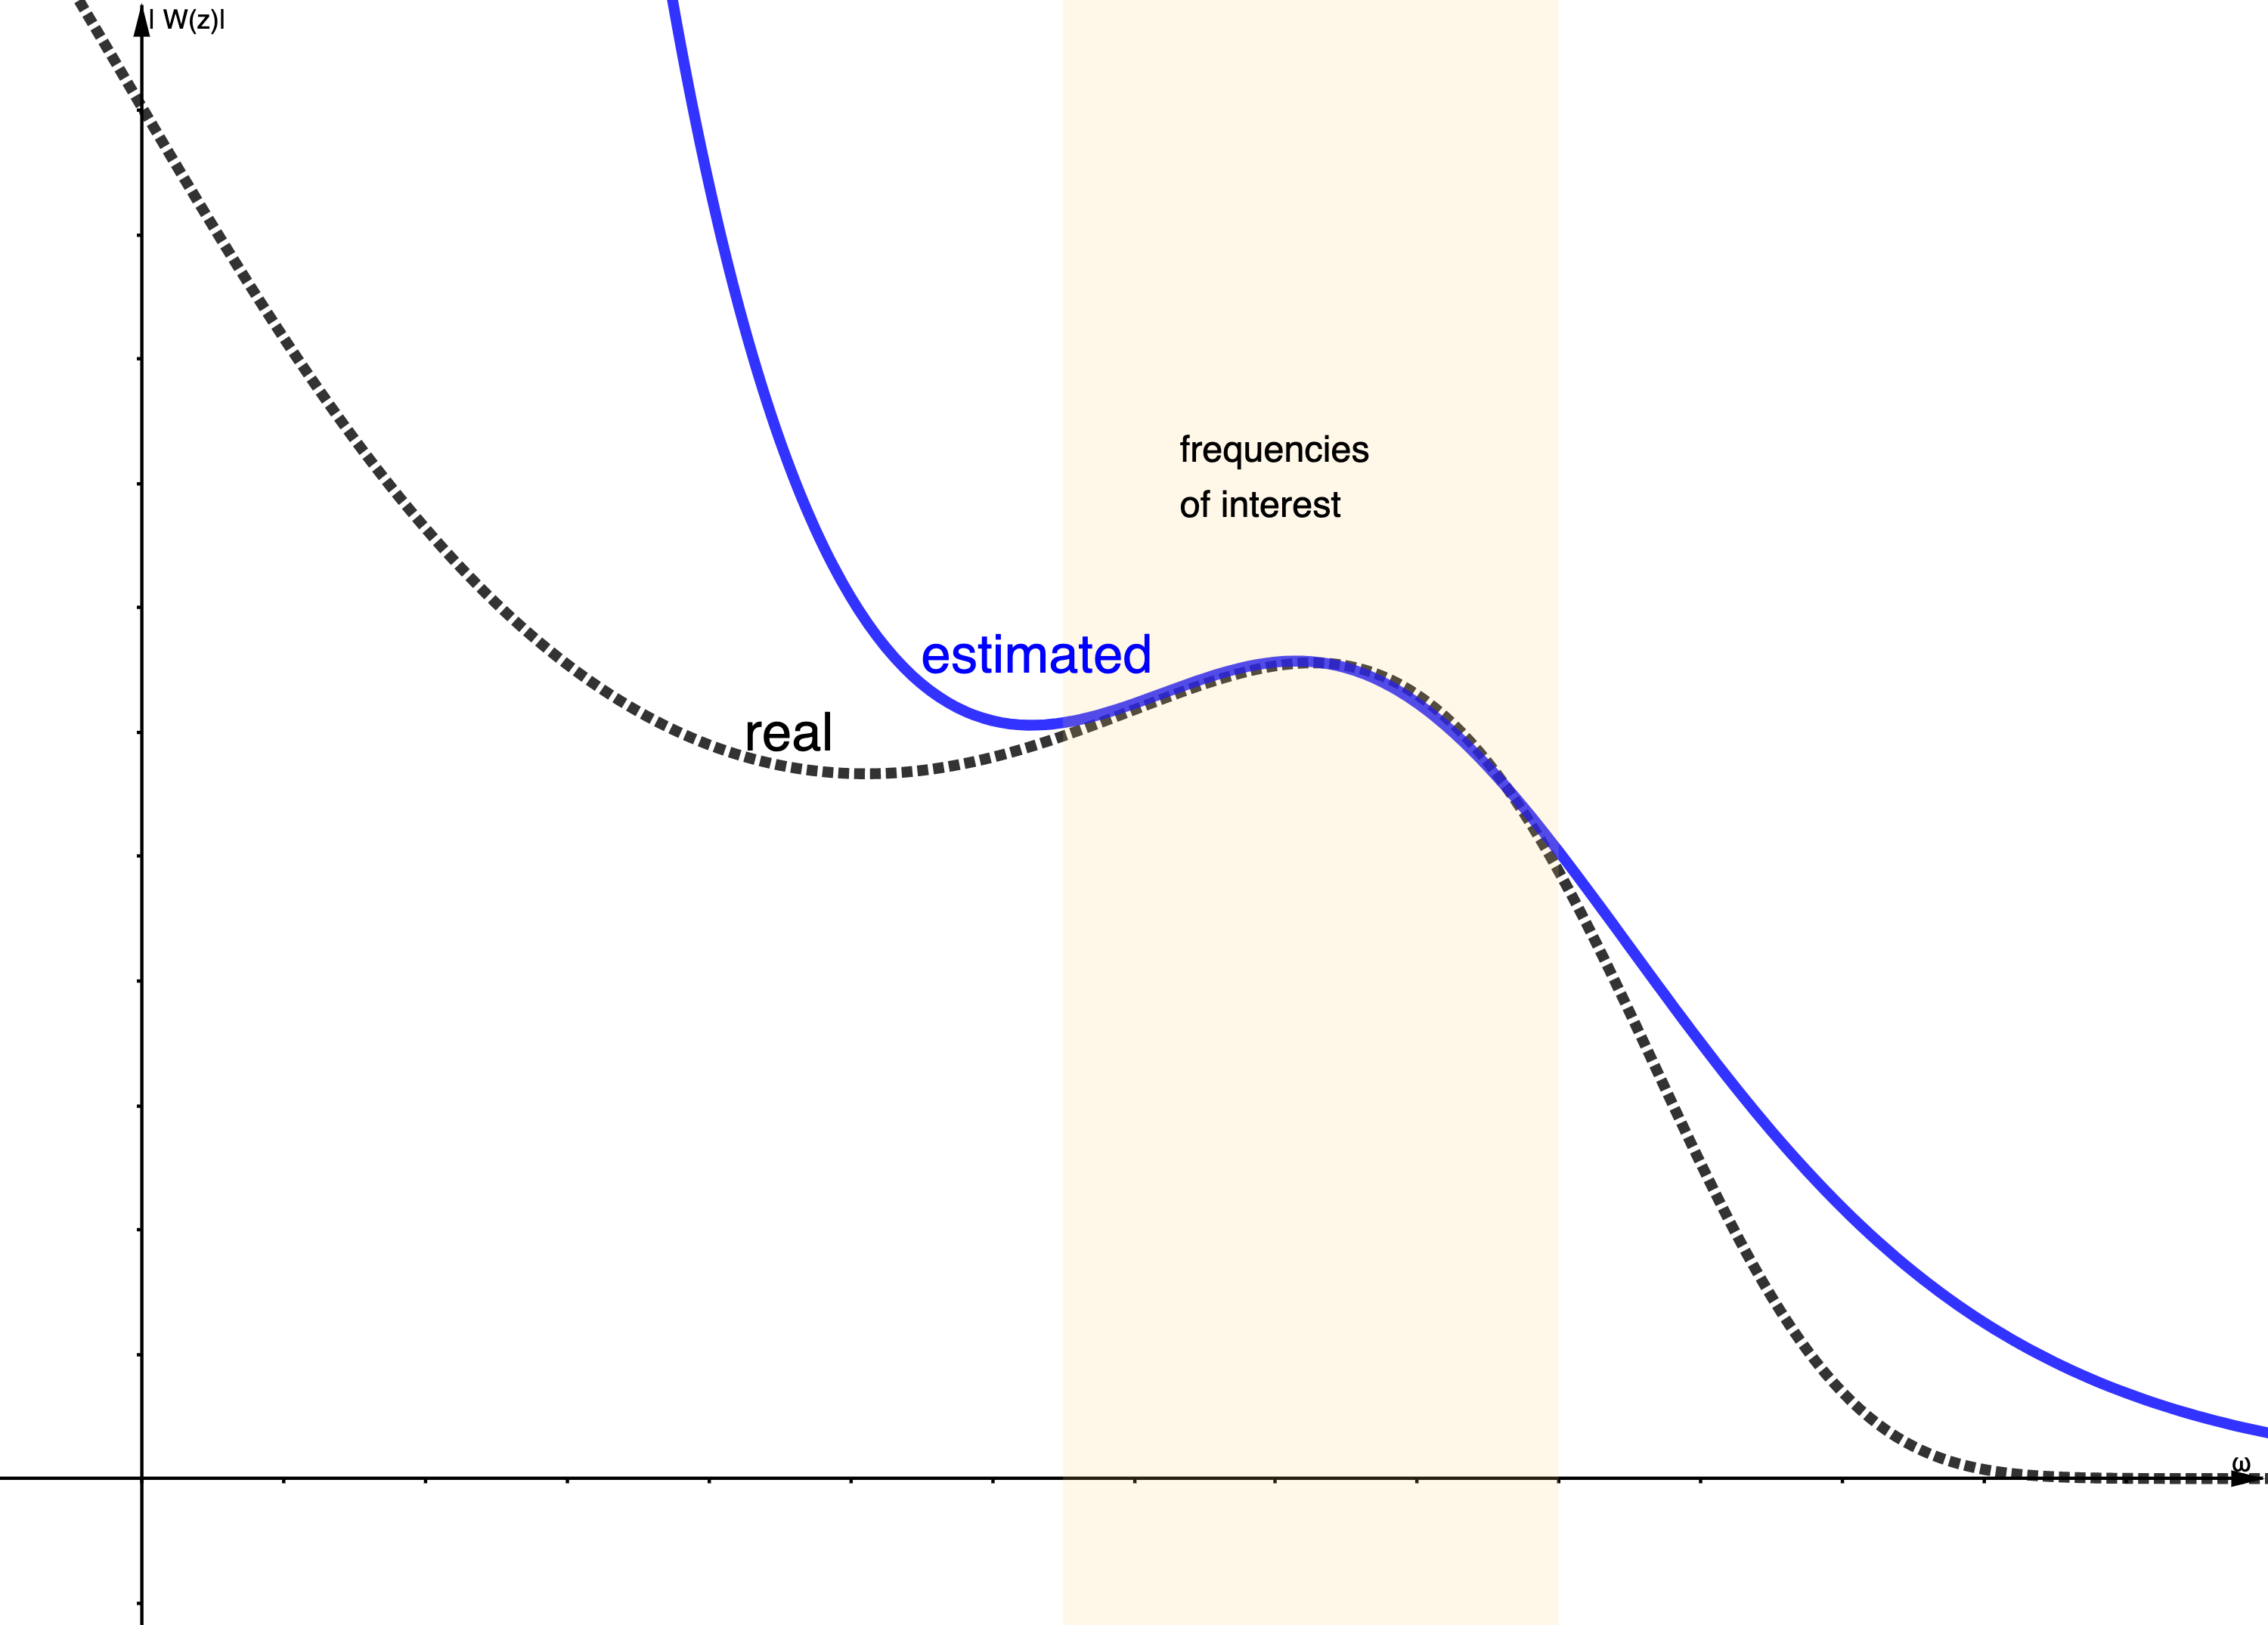
\includegraphics[scale=4.5]{./img/freq-emphasis.png}
    \end{figure}

    We can manage this selected focus on estimation precision using non-uniform weights $\lambda_i$ (different weights for different frequencies).

    \begin{figure}[H]
        \centering
        \begin{tikzpicture}[node distance=2.5cm,auto,>=latex']
            \begin{axis}[axis lines=none,ymax=2.5]
                \addplot[color=blue,mark=square]
                    coordinates {
                        (0,1)(1,1)(2,1)(3,1.2)(4,2)(5,1.2)(6,1)(7,1)(8,1)
                    };
            \end{axis}

            \draw[->] (-0.5,0) -- (7,0) node[right] {$\omega$};
            \draw[->] (0.5,-0.5) -- (0.5,5) node[left] {$\lambda_i$};
            \node at (0.1,0.5) {$1$};
            \draw (6.3,0.1) -- (6.3,-0.1) node [below] {$\omega_H$};
            \draw (1.3,0.1) -- (1.3,-0.1) node [below] {$\omega_1$};
            \draw (2,0.1) -- (2,-0.1) node [below] {$\omega_2$};
            \draw (3.5,0.1) -- ++(0,-0.2) node [below] {$\omega_x$};
        \end{tikzpicture}
    \end{figure}
    
    where $\omega_x$ is the frequency of interest.
    
    
    The performance index can be redefined:
    \[
        \tilde{J}_H (\theta) = \frac{1}{H} \sum_{i=1}^H \lambda_i \left(W(e^{j\omega_i};\theta) - \frac{\hat{B}_i}{A_i}e^{j\hat{\phi}_i}\right)^2
    \]

    Another \emph{trick}: more dense $\omega_i$ spacing in the frequency region of special interest (not really used).
\end{remark}

\begin{remark}[Single experiment]
    Sometimes the set of $H$ independent single-sinusoid experiments can be replaced by a long single ``sine-sweep'' experiment, that is to measure the frequency response of the system when the input is sinusoid that starts with frequency $\omega_1$ and amplitude $A_1$ and ends with frequency $\omega_H$ and amplitude $A_H$. 

    \begin{figure}[H]
        \centering
        \begin{tikzpicture}[node distance=2.5cm,auto,>=latex']
            \draw[->] (-0.5,0) -- (5,0) node[right] {$t$};
            \draw[->] (0,-1) -- (0,2) node[left] {$u(t)$};
            \draw[domain=0:4.5,samples=100,smooth,variable=\x,blue] plot ({\x},{cos(\x*180/3.14*(\x^1.7+5))*e^(-\x/2.5)});
        \end{tikzpicture}
        \caption*{Slowing-varying sinusoid with increasing frequency and decreasing amplitude.}
    \end{figure}

    The output will be a single long signal $y(t)$.
    
    We can cut a-posteriori the signal into $H$ pieces, and then back to the standard procedure
    or we can directly compute an estimation of $\hat{W}(e^{j\omega})$ as a ration of the output and input spectra %(recalling that $\Gamma_y(\omega) = |W(z)|^2 \Gamma_u(\omega)$)

    \[
        \hat{W}(e^{j\omega}) = \frac{\hat{\Gamma}_y(e^{j\omega})}{\hat{\Gamma}_u(e^{j\omega})}
    \]

    We can fit the estimated $\hat{W}(e^{j\omega})$ with the model frequency response $W(e^{j\omega}; \theta)$ in the performance index.
    
    \[
        \frac{1}{H} \sum_{i=1}^H \left| W(e^{j \omega_i}; \theta) - \hat{W}(e^{j \omega_i}) \right|^2
    \]
    where, similarly, $W(e^{j\omega_i}; \theta)$ is the modeled frequency response and $\hat{W}(e^{j \omega_i})$ is the measured frequency response.
    
    This experiment is quicker but has usually a lower signal-to-noise-ration.
\end{remark}

\begin{remark}[Experiment on unstable system]
    What happen if the system is \emph{open-loop} unstable? We have to stop the experiment because of the instability of the output (which of course diverges).
    
    \begin{figure}[H]
    \centering
    \begin{tikzpicture}[node distance=1.5cm,auto,>=latex']
        \node[block] (sys) {$\Sys$};
        \node[left of=sys, node distance=3cm] (in) {};
        \node[left of=in] (in2) {};
        \node[right of=sys, node distance=2.5cm] (out) {};
        \node[right of=out, node distance=2cm] (out2) {};

        \draw[xshift=-4cm,yshift=0.5cm,scale=0.2,domain=0:4*pi,smooth,variable=\x] plot ({\x},{sin(8*\x r)});

        \draw[xshift=1cm,yshift=0.5cm,scale=0.2,domain=0:4*pi,smooth,variable=\x,samples=100] plot ({\x},{sin(8*\x r + 10)*exp(0.15*\x)});
        \draw[->] (in2) -- (sys);
        \draw[->] (sys) -- (out2);
    \end{tikzpicture}
\end{figure}
    
    We can avoid this problem by performing the experiment in \emph{closed-loop}  and adding a \emph{stability controller}.
    
        \begin{figure}[H]
        \centering
        \begin{tikzpicture}[node distance=2.5cm,auto,>=latex']
            \node [block,align=center] (stab) {stability\\controller};
            \node [block] (sys) [right of=sum, node distance=2cm]{$\Sys$};
            \node [coordinate] (split) [right of=sys, node distance=1cm]{};
            \node [] (end) [right of=split, node distance=3cm]{$y(t)$};
            \node [] (in) [left of=stab, node distance =4cm]{$\bar{y}(t)$};
            \node [coordinate] (mid) [below of=sum, node distance=1.5cm] {};

            \draw[->] (in) -- (stab);
            \draw[->] (stab) -- (sys);
            \draw (sys) edge (split);
            \draw[->] (split) -- (end);
            \draw (split) |- (mid);
            \draw[->] (mid) -| (stab);
            
            \draw[xshift=-3.6cm, yshift=0.5cm, scale=0.2, domain=0:4*pi, smooth, variable=\x] plot ({\x}, {sin(8*\x r)});
            \draw[blue, xshift=1cm, yshift=0.5cm, scale=0.2, domain=0:4*pi, smooth, variable=\x] plot ({\x}, {1.5*sin(8*\x r + 5)});
            \draw[blue, xshift=4.5cm, yshift=0.5cm, scale=0.2, domain=0:4*pi, smooth, variable=\x] plot ({\x}, {0.7*sin(15*\x r + 7)});
            
        \end{tikzpicture}
    \end{figure}
    
    where the blue sinusoids are the signal reflecting the dynamic of the system and, measuring them, they will compose the dataset I/O of the system. 
    
    \textbf{Note} that the model identified using that dataset will be a model of an unstable system.
    
    This is just a trick to collect data from an unstable system.
\end{remark}



\section{Comparison between time domain and frequency domain parametric methods}

\paragraph{Frequency domains}
\begin{description}
    \item[Pro] Robust and very reliable because each experiment has a big signal-to-noise ratio (since we are forcing all the signal energy on a single clean sinusoid).
    \item[Pro] Intuitive since it is easy to understand.
    \item[Pro] Consistent with many control-design methods that work in the frequency domain.
    \item[Cons] More demanding in terms of design of the experiment.
    \item[Cons] Provides no noise model (unlike the \gls{pem} method of \gls{armax} system identification)
    \end{description}

\textbf{Note} that F.D. and T.D. methods should provide approximately the same result if done correctly.


\chapter{Software (virtual) Sensing model-based in feedback method using Kalman Filter framework}

In MIDA1 we have mostly used I/O \acrfull{tf} representations:
\[ y(t) = \frac{B(z)}{A(z)}u(t-k) + \frac{C(z)}{A(z)}e(t) \qquad e(t) \sim \WN \]


Kalman filter theory is fully based on \acrfull{ss} representation

\[
    \begin{cases}
        x(t+1) = Fx(t) + Gu(t) + v_1(t)  & \qquad v_1 \sim \WN \\
        y(t) = Hx(t) + \cancel{Du(t)} + v_2(t) & \qquad v_2 \sim \WN
    \end{cases}
\]

where we assume that the system model is given (typically obtained in a white-box approach): it's not a system identification problem! Indeed we are interested in the internal state of the system.

\begin{figure}[H]
    \centering
    \begin{tikzpicture}[node distance=2.5cm,auto,>=latex']
        \node [block, align=center] (sys) {$\Sys$ \\ \vspace{10pt} \qquad \\ \qquad$x(t)$};
        \node (in) [left of=sys, node distance=2cm] {$u(t)$};
        \node (out) [right of=sys, node distance=2cm]{$y(t)$};
        \node (wn1) [above of=sys, node distance=1.5cm, xshift=-1cm] {$v_1(t)$};
        \node (wn2) [above of=sys, node distance=1.5cm, xshift=1cm] {$v_2(t)$};

        \draw[->] (in) -- (sys);
        \draw[->] (sys) -- (out);
        \draw[->] (wn1) -- (sys);
        \draw[->] (wn2) -- (sys);
    \end{tikzpicture}
    \caption*{Two-noises model}
\end{figure}


\section{Motivation and Goals of Kalman Filter (KF)}

Given a model description $\{F, G, H\}$ and noises variances (not a system identification technique), with \acrfull{kf} theory we can address the following problems:

\begin{itemize}
    \item Find the $k$-steps ahead prediction of output: $\hat{y}(t+k|t)$ (already solved in MIDA1 with \gls{armax}).
    \item Find the $k$-steps ahead prediction of state: $\hat{x}(t+k|t)$.
    \item Find the filter of the state at present time: $\hat{x}(t|t)$. In practice it's a \emph{software-sensing} problem, which is the most important problem solved by Kalman filter (reason of why it is named Kalman \emph{filter}).
    \item Gray box system identification (see \nameref{ch5}). We have a recorded data-set and the model structure with some unknown parameters.
\end{itemize}



%!TEX root = ../main.tex

Dynamical systems have this layout:

\begin{figure}[H]
    \centering
    \begin{tikzpicture}[node distance=2.5cm,auto,>=latex']
        \node [block, align=center] (sys) {$x_1(t)$\\$x_2(t)$\\$\vdots$\\$x_n(t)$};
        \node (in1) [left of=sys, node distance=2cm, yshift=0.7cm] {$u_1(t)$};
        \node (in2) [left of=sys, node distance=2cm] {$u_2(t)$};
        \node (dots1) [left of=sys, node distance=2cm, yshift=-0.5cm]{$\vdots$};
        \node (in3) [left of=sys, node distance=2cm, yshift=-1cm] {$u_m(t)$};
        \node (out1) [right of=sys, node distance=2cm, yshift=0.7cm]{$y_1(t)$};
        \node (out2) [right of=sys, node distance=2cm]{$y_2(t)$};
        \node (dots2) [right of=sys, node distance=2cm, yshift=-0.5cm]{$\vdots$};
        \node (out3) [right of=sys, node distance=2cm, yshift=-1cm]{$y_p(t)$};

        \draw[->] (in1) -- (sys);
        \draw[->] (in2) -- (sys);
        \draw[->] (in3) -- (sys);
        \draw[->] (sys) -- (out1);
        \draw[->] (sys) -- (out2);
        \draw[->] (sys) -- (out3);
    \end{tikzpicture}
\end{figure}

where, in this case, the system is MIMO: it has $m$ inputs (actuators/control variables), $p$ outputs (sensors) and $n$ states.

\textbf{Key problem} usually $p \ll n$, that is, physical sensors are much less than system states, because of:
\begin{itemize}
    \item cost
    \item cables, power supply, installation
    \item maintenance (faults, degradation)
    \item existence of such sensors
\end{itemize}

That's why usually not all the states are measured (available). However, it is very useful to have full ``measurement'' of states because:
\begin{itemize}
    \item design of control algorithms (state feedback design)
    \item monitoring of the system (fault detection, predictive maintenance, \dots)
\end{itemize}

This problem can be solved with \emph{software sensing (SW-sensing)} (also called virtual sensing) algorithms:
\begin{figure}[H]
    \centering
    \begin{tikzpicture}[node distance=2.5cm,auto,>=latex']
        \node [block, align=center] (sys) {$\Sc$\\\qquad$x(t)$};
        \node (in1) [left of=sys, node distance=2cm, yshift=0.7cm] {};
        \node (in2) [left of=sys, node distance=2.3cm] {$u(t)$};
        \node (in3) [left of=sys, node distance=2cm, yshift=-0.7cm] {};
        \node (out1) [right of=sys, node distance=2cm, yshift=0.7cm]{};
        \node (out2) [right of=sys, node distance=2.3cm]{$y(t)$};
        \node (out3) [right of=sys, node distance=2cm, yshift=-0.7cm]{};

        \node [block, align=center, below of=sys] (algo) {SW-sensing algorithm};
        \node (algoout) [right of=algo, node distance=3cm] {$\hat{x}(t)$};
        
        \draw[<-, dashed] (sys.north) --++ (0,1)
            node[right, align=center] {immeasurable \\ disturbances};
        \draw[->] (in1) -- (sys);
        \draw[->] (in2) -- (sys);
        \draw[->] (in3) -- (sys);
        \draw[->] (sys) -- (out1);
        \draw[->] (sys) -- (out2);
        \draw[->] (sys) -- (out3);

        \draw[->] (-1.4,0.8) -- (-1.4,-1) -- (algo);
        \draw[->] (1.4,0.8) -- (1.4,-1) -- (algo);
        \draw[->] (algo) -- (algoout);
    \end{tikzpicture}
\end{figure}

where $\hat{x}(t)$ is an estimation (or SW-sensing) of the internal state $x(t)$.

\paragraph{Designer Dilemma} When using software sensing and when physical sensing?
\begin{itemize}
    \item In some cases there is no option (not feasible installation of a physical sensor)
    \item In most cases both options are viable: variable vs fixed cost
\end{itemize}

\begin{figure}[H]
    \centering
    \begin{tikzpicture}[node distance=2.5cm,auto,>=latex']
        \draw[->] (-0.5,0) -- (4,0) 
            node[right, align=center] {Fixed development costs\\of software sensing algorithm}
            node[right, above] {€}; 
        \draw[->] (0,-0.5) -- (0,4) 
            node[left, align=right] {Variable cost proportional\\to the number of sensors}
            node[above, right] {€};
        \draw[domain=0:2.5,samples=20,smooth,variable=\x,red] plot ({\x},{sqrt(2.5^2-\x^2)});
        
        \draw[red] (-0.1,2.5) --++ (0.2, 0) node[left, xshift=-0.2cm] {\color{red} break-even};
        \draw (2.5,0.1) --++ (0, -0.2) node[below] {$c$};
        
        \draw [decorate,decoration={brace,amplitude=10pt}] (0,0) -- (0,2.5) node [black,midway,align=right,xshift=-0.3cm] {Low volumes production:\\better physical sensing};
        \draw [decorate,decoration={brace,amplitude=7pt}] (0,3.5) -- (0,2.5) node [black,midway,align=left,xshift=0.3cm] {High volumes production:\\better software sensing};
    \end{tikzpicture}
    \caption*{Break-even analysis}
\end{figure}

Given $c$, the fixed cost of development of the software sensor, it is possible to compute the break-event point.
The break-even point coincides with the number of products such that above that number it is more convenient to use software sensing, while below that number it is more convenient to buy and install physical sensors per each product.

Anyway, in some cases we might use both physical and software sensing for redundancy (e.g. in very safety-critical or mission-critical applications).

\paragraph{Key questions for software sensing}

\begin{itemize}
    \item Is software-sensing feasible? Test is the observability of the states from measured outputs (through physical sensors).
    \item If feasible, check if the level of noise (error) of the estimated variable is acceptable.
\end{itemize}

\begin{exa}[Slip estimation for ABS/traction control]
Now we go back to the ABS example (described in \ref{abs_ex}) where we realized that SW-sensing is needed for the estimation of $v$, the horizontal velocity of the car, since it cannot be measured with a physical sensor.
    \begin{figure}[H]
        \centering
        \begin{tikzpicture}[node distance=1.5cm,auto,>=latex']
            \draw (0.5,0) -- (0,0) -- (0,0.5) -- (1,0.5) -- (1.5,1) -- (2.5,1) -- (2.8,0.5) -- (3.3,0.5) -- (3.3,0) -- (3.1,0);
            \draw (1.1,0) -- (2.5,0);
            \draw (0.8,0) circle (0.3);
            \draw (2.8,0) circle (0.3);

            \draw[->] (-0.1,0.5) -- (-0.6,0.5) node[left] {$v$};
            \draw[->] (0.8,0) -- (0.8,-0.3) node[below] {$r$};
            \draw[->] (1.146,0.2) arc[radius=0.4, start angle=30, end angle=90];
            \node at (1.3,0.5) {$\omega$};
        \end{tikzpicture}
    \end{figure}

    
    Indeed, measure of $v$ cannot be done with an optical sensor or a GPS:
    they both have a problem of availability (not guaranteed). Physical sensing is not an option for industrial production.

    Intuitive solution: install a longitudinal accelerometer ($a_x$) and integrate.
    \begin{figure}[H]
        \centering
        \begin{tikzpicture}[node distance=1.5cm,auto,>=latex']
            \draw (0.5,0) -- (0,0) -- (0,0.5) -- (1,0.5) -- (1.5,1) -- (2.5,1) -- (2.8,0.5) -- (3.3,0.5) -- (3.3,0) -- (3.1,0);
            \draw (1.1,0) -- (2.5,0);
            \draw (0.8,0) circle (0.3);
            \draw (2.8,0) circle (0.3);

            \draw[->] (2.3,0.5) -- (1.7,0.5) node[above] {$a_x$};
        \end{tikzpicture}
    \end{figure}
    \[
        \hat{v} = \int a_x(t) dt \qquad \iff \qquad a_x(t) \rightarrow 1/s \rightarrow \hat{v}(t)
    \]

    In discrete time domain: discretization using approximation of derivative, Eulero forward method (see \nameref{appendix:discr})
    \[
        \frac{d}{dt} v(t) = a_x(t) \qquad \frac{dv(t)}{dt} \approx \frac{v(t+1)-v(t)}{\Delta T_s} = a_x(t)
    \]

    Where $\Delta T_s$ is the sampling interval (e.g. 10ms).

    \[
        \hat{v}(t) = \hat{v}(t-1) + \Delta T_s a_x(t-1)
    \]

    \begin{figure}[H]
        \centering
        \begin{tikzpicture}[node distance=2.5cm,auto,>=latex']
            \node [block] (sys) {$\frac{\Delta T_s}{1-z^{-1}}$};
            \node (in) [left of=sys, node distance=2cm] {};
            \node (end) [right of=sys, node distance=2cm]{};

            \draw[->] (in) edge node {$a_x(t)$} (sys);
            \draw[->] (sys) edge node {$\hat{v}(t)$} (end);
        \end{tikzpicture}
    \end{figure}

    Unfortunately the measured signal is not $a_x(t)$ but $a_x(t)+d_{a_x}(t)$.

    \begin{figure}[H]
        \centering
        \begin{tikzpicture}[node distance=2.5cm,auto,>=latex']
            \begin{axis}[axis lines=none,ymax=6]
                \addplot[color=blue,smooth]
                    coordinates {
                        (0.00,2.35)(0.40,2.87)(0.80,2.99)(1.20,2.75)(1.60,2.83)(2.00,2.86)(2.40,3.19)(2.80,2.76)(3.20,2.45)(3.60,2.85)(4.00,2.55)(4.40,2.50)(4.80,2.64)(5.20,2.72)(5.60,3.26)(6.00,3.68)(6.40,3.95)(6.80,3.9)(7.20,4.00)(7.60,3.51)
                    };
                \addplot[color=red,smooth]
                    coordinates {
                        (0.00,2.35)(0.40,2.91)(0.80,3.07)(1.20,2.87)(1.60,2.99)(2.00,3.06)(2.40,3.43)(2.80,3.04)(3.20,2.77)(3.60,3.21)(4.00,2.95)(4.40,2.94)(4.80,3.12)(5.20,3.24)(5.60,3.82)(6.00,4.28)(6.40,4.59)(6.80,5.17)(7.20,5.0)(7.60,5.27)
                    };
                \draw[->] (-0.5,0) -- (800,0) node[right] {$t$};
                \draw[->] (0.5,-0.5) -- (0.5,300) node[left] {};
            \end{axis}
        \end{tikzpicture}
    \end{figure}

    Integrating noise generates a \emph{drift}. Integrator is not an asymptotic stable system.

    \begin{figure}[H]
        \centering
        \begin{tikzpicture}[node distance=2.5cm,auto,>=latex']
            \node [block] (sys) {$\frac{\Delta T_s}{1-z^{-1}}$};
            \node [sum] (in) [left of=sys, node distance=1.5cm] {};
            \node (in1) [above of=in, node distance=1cm] {$d_{a_x}(t)$};
            \node (in2) [below of=in, node distance=1cm] {$a_x(t)$};
            \node (end) [right of=sys, node distance=2cm]{};

            \draw[->] (in) -- (sys);
            \draw[->] (in1) -- (in) node[left, pos=0.8] {$+$};
            \draw[->] (in2) -- (in) node[left, pos=0.8] {$+$};
            \draw[->] (sys) edge node {$\hat{v}(t)$} (end);
        \end{tikzpicture}
    \end{figure}

    \paragraph{Solution} Use a Kalman Filter.

    \begin{figure}[H]
        \centering
        \begin{tikzpicture}[node distance=2.5cm,auto,>=latex']
            \node [block, align=center, minimum width=3cm] (sys) {car};
            \node [block, align=center, minimum width=3cm, below of=sys] (algo) {Kalman Filter};
            \node (algoout) [right of=algo, node distance=3cm] {$\hat{v}(t)$};

            \draw[->,transform canvas={xshift=-1.2cm}] (sys) -- (algo) node[pos=0.5] {$\omega_1$};
            \draw[->,transform canvas={xshift=-0.6cm}] (sys) -- (algo) node[pos=0.5] {$\omega_2$};
            \draw[->] (sys) -- (algo) node[pos=0.5] {$\omega_3$};
            \draw[->,transform canvas={xshift=0.6cm}] (sys) -- (algo) node[pos=0.5] {$\omega_4$};
            \draw[->,transform canvas={xshift=1.2cm}] (sys) -- (algo) node[pos=0.5] {$a_x$};

            \draw[->] (algo) -- (algoout);
        \end{tikzpicture}
    \end{figure}
\end{exa}

\begin{exa}[State of charge estimation of a battery]
    \begin{figure}[H]
        \centering
        \begin{tikzpicture}[node distance=2.5cm,auto,>=latex']
            \draw (0,0) rectangle ++(1.5cm,3cm);
            \draw (0.6cm,3cm) rectangle ++(0.3,0.15);

            \draw [pattern=north west lines, pattern color=green] (0,0) rectangle (1.5,2);

            \draw [decorate,decoration={brace,amplitude=10pt}] (0,0) -- (0,3) node [black,midway,align=right,xshift=-0.3cm] {100\%};
            \draw [decorate,decoration={brace,amplitude=10pt}] (1.5,2) -- (1.5,0) node [black,midway,align=right,xshift=0.3cm] {SoC};

            \node [block, align=center] (sys) at (6,1.5) {SoC\\internal\\state};
            \node [left of=sys, node distance=2cm] (in1) {$i(t)$};
            \node [above of=sys, node distance=2cm] (in2) {$T(t)$};
            \node [right of=sys, node distance=2cm] (out) {$v(t)$};

            \draw[->] (in1) -- (sys);
            \draw[->] (in2) -- (sys);
            \draw[->] (sys) -- (out);
        \end{tikzpicture}
    \end{figure}
    \[
        \text{SoC}(t) = 1 - \frac{\int i(t)dt}{I} \qquad 0 \le \text{SoC} \le 1
    \]
    Where $I$ is the total amount of \emph{current} that can be extracted by the user of the battery.
    This solution is not feasible since it integrates the noise on $i(t)$.
\end{exa}

\section{Kalman Filter on Basic Systems}

\begin{itemize}
    \item No external inputs ($\cancel{Gu(t)}$): time series
    \item Linear systems
    \item Time invariant systems
\end{itemize}

The basic solution of this basic system is the 1-step prediction.\\
After that, we will make the extensions to more general systems:
\begin{itemize}
    \item k-step prediction
    \item filter $\hat{x}(t|t)$
    \item time-varying systems
    \item systems with exogenous inputs (presence of ${Gu(t)}$)
    \item non-linear systems (Extended Kalman Filter (EKF))
\end{itemize}

\subsection{Detailed description of Basic System}

The basic system we initially consider is a MIMO system with $n$ states, ($m$ inputs) and $p$ outputs.

\[
    \Sc: \begin{cases}
        x(t+1) = Fx(t) + \cancel{Gu(t)} + v_1(t) & \text{state equation}\\
        y(t) = Hx(t) + \cancel{Du(t)} + v_2(t) & \text{output equation}
    \end{cases}
\]
\[
    x(t) = \begin{bmatrix}
        x_1(t) \\
        x_2(t) \\
        \vdots \\
        x_n(t)
    \end{bmatrix}
    \qquad
    \left(\;u(t) = \begin{bmatrix}
        u_1(t) \\
        u_2(t) \\
        \vdots \\
        u_m(t)
    \end{bmatrix}\;\right)
    \qquad
    y(t) = \begin{bmatrix}
        y_1(t) \\
        y_2(t) \\
        \vdots \\
        y_p(t)
    \end{bmatrix}
\]

\begin{description}
    
    \vspace{15pt}
    
    \item [State Noise] $v_1(t)$ is a vector white-noise.
    \[
        v_1(t) \sim \WN(0, V_1) \qquad v_1(t) = \begin{bmatrix}
            v_{11}(t) \\
            v_{12}(t) \\
            \vdots \\
            v_{1n}(t)
        \end{bmatrix}
    \]
    
    and it is called \emph{state noise} or \emph{model noise}.
    It is used to model immeasurable noises affecting the system and small modelling errors.
    
    \textbf{Properties of $v_1(t)$}:
    \begin{enumerate}
        \item $\EE[v_1(t)] = \vec{0}$
        \item $\EE[v_1(t) \cdot v_1\transpose(t)] = V_1$, where $V_1$ is an $n\times n$ covariance matrix (square, symmetric and semi-definite positive by definition)
        \item $\EE[v_1(t) \cdot v_1\transpose(t-\tau)] = [0]_{n \times n} \quad \forall t \quad \forall \tau \ne 0$ (\emph{whiteness} property)
    \end{enumerate}
    
    \vspace{15pt}
    
    \item [Output Noise] $v_2(t)$ is a vector white-noise.
    \[
        v_2(t) \sim \WN(0, V_2) \qquad v_2(t) = \begin{bmatrix}
            v_{21}(t) \\
            v_{22}(t) \\
            \vdots \\
            v_{2p}(t)
        \end{bmatrix}
    \]
    
    and it is called \emph{output noise} or \emph{sensor noise}. It is the noise affecting the output sensor measurements.
    
    \textbf{Properties of $v_2(t)$}:
    \begin{enumerate}
        \item $\EE[v_2(t)] = \vec{0}$
        \item $\EE[v_2(t) \cdot v_2\transpose(t)] = V_2$, where $V_2$ is a $p\times p$ covariance matrix (square, symmetric and semi-definite positive\footnote{We make the \textbf{assumption that $V_2$ is definite positive} (i.e. $V_2 > [0]_{n \times p}$) because we will need this property in the Riccati equation.} by definition)
        \item $\EE[v_2(t) \cdot v_2\transpose(t-\tau)] = [0]_{n \times n} \quad \forall t \quad \forall \tau \ne 0$ (\emph{whiteness} property)
    \end{enumerate}

\end{description}

\textbf{Assumptions} about the relationships between $v_1(t)$ and $v_2(t)$:
\[
    \EE[v_1(t) \cdot v_2\transpose(t-\tau)] = \begin{cases} \label{sys:corrV12} \tag*{$\clubsuit$}
        [0]_{n \times p} & \text{if } \tau \ne 0 \\
        V_{12} & \text{if } \tau = 0
    \end{cases}
\]

where $V_{12}$ is a cross-correlation matrix of size $n\times p$.

The system \eqref{sys:corrV12} means that $v_1$ and $v_2$ can be correlated only at the same time, but, in practice, $V_{12}=0$ is the most common assumption. Thus, in practice

\[\EE[v_1(t) \cdot v_2\transpose(t-\tau)] = [0]_{n \times p} \quad \forall t \forall \tau  \qquad \qquad \text{($1^{st}$ assumption)} \]

Since the system $\Sc$ is dynamic we need to define the (in this case, probabilistic) initial conditions:
\[
    \EE[x(1)] = \underbrace{X_0}_{n\times 1} \qquad \EE[\left(x(1) - X_0)\right)\left(x(1)-X_0\right)\transpose] = \underbrace{P_0}_{n\times n} \ge [0]_{n \times n}
\]

If the covariance matrix $P_0 = [0]_{n \times n}$ the initial state is perfectly known.

Finally we assume that the two noises $v_1(t)$ and $v_2(t)$ are uncorrelated with the initial state:
\[
    x(1) \perp v_1(t) \qquad x(1) \perp v_2(t) \qquad \qquad \text{($2^{nd}$ assumption)}
\]

\textbf{Note} From now on, \emph{null matrices} $[0]_{n \times m}$ will be simply denoted by $0$. 

\subsection{KF Basic Solution of the Basic System}\label{subsec:KF-basic_sol}

%\renewcommand\nameeq[2]{\phantom{\text{#2}}&&#1&&\text{#2}}

\begin{flalign}\label{eq:KF-state}
    \nameeq{\hat{x}(t+1|t) = F\hat{x}(t|t-1) + K(t)e(t)}{State eq.}
\end{flalign}    

\begin{flalign}\label{eq:KF-out}    
    \nameeq{\hat{y}(t|t-1) = H\hat{x}(t|t-1)}{Output eq.}
\end{flalign} 

\begin{flalign}\label{eq:KF-pred-err}    
    \nameeq{e(t) = y(t) - \hat{y}(t|t-1)}{Prediction output error eq.}
\end{flalign} 

\begin{flalign}\label{eq:KF-gain}    
    \nameeq{K(t) = \left( FP(t)H\transpose+V_{12} \right) \left( HP(t)H\transpose+V_2 \right)^{-1}}{Gain of the filter}
\end{flalign} 

\begin{flalign}\label{eq:KF-DRE}    
    \nameeq{P(t+1) = \left( FP(t)F\transpose + V_1 \right) - \left( FP(t)H\transpose + V_{12} \right)\left( HP(t)H\transpose + V_{2} \right)^{-1}\left( FP(t)H\transpose + V_{12} \right)\transpose}{\acrshort{dre}}
\end{flalign}  
    
%\begin{align*}
%    & \hat{x}(t+1|t) = F\hat{x}(t|t-1) + K(t)e(t) && \qquad \text{state equation} \\
%    & \hat{y}(t|t-1) = H\hat{x}(t|t-1) &&\qquad \text{output equation} \\
%    & e(t) = y(t) - \hat{y}(t|t-1) &&\qquad \text{output prediction error} \\
%    & K(t) = \left( FP(t)H\transpose+V_{12} \right) \left( HP(t)H\transpose+V_2 \right)^{-1} &&\qquad \text{gain of the K.F.} \\
%    & P(t+1) = \left( FP(t)F\transpose + V_1 \right) + &&\\
%    & - \left( FP(t)H\transpose + V_{12} \right)\left( HP(t)H\transpose + V_{2} \right)^{-1}\left( FP(t)H\transpose + V_{12} \right)\transpose && \qquad\text{difference Riccati equation}
%\end{align*}

Since \ref{eq:KF-state} and \ref{eq:KF-DRE} are dynamical equations, two initial conditions are needed:

\begin{flalign}\label{eq:KF-initCond-state}    
    \nameeq{\hat{x}(1|0) = \EE[x(1)] = X_0}{Init. condition for \ref{eq:KF-state}}
\end{flalign}  

\begin{flalign}\label{eq:KF-initCond-DRE}    
    \nameeq{P(1) = \text{var}[x(1)] = P_0}{Init. condition for \ref{eq:KF-DRE}}
\end{flalign}  

\begin{defn}[Difference Riccati Equation (DRE)]
    The equation \ref{eq:KF-DRE} is called \emph{\acrfull{dre}} and it is a special type of non-linear matrix difference equation. 
    
    \quad \textbf{Note} The \gls{dre} is an autonomous (i.e. there are no inputs), non-linear, discrete time, multi-variable system, described by a non-linear difference matrix equation
    \[
         P(t+1) = f_{NL}(P(t)) \qquad P(1) = P_0
    \]
\end{defn}


\begin{rem}[Structure or $K(t)$ and \gls{dre}]
    Notice that $K(t)$ and the \gls{dre} have  a \emph{block-structure} having this form: 
    
    \[ AP(t)B\transpose+N  \qquad \text{where $N$ is a noise matrix}\]

    There are 3 different types of blocks:
    \begin{align*}
        \texttt{state:} \qquad& FP(t)F\transpose+V_1 \qquad\text{\small{(since $F$ refers to \ref{eq:KF-state})}}\\
        \texttt{output:} \qquad& HP(t)H\transpose+V_2 \qquad\text{\small{(since $H$ refers to \ref{eq:KF-out})}}\\
        \texttt{mix:} \qquad& FP(t)H\transpose+V_{12}
    \end{align*}

    Therefore
    \begin{align*}
        \text{\ref{eq:KF-gain} becomes:} \qquad& K(t) \equiv (\texttt{mix})(\texttt{output})^{-1} \\
        \text{\ref{eq:KF-DRE} becomes:} \qquad& P(t+1) \equiv (\texttt{state}) - (\texttt{mix})(\texttt{output})^{-1}(\texttt{mix})\transpose
    \end{align*}
\end{rem}


\begin{rem}[Existance of the \gls{dre}]
    In order to guarantee the existance of the \gls{dre} for all time instant $t$, the only critical part is the inversion of the \texttt{output} block:
    \[
        \underbrace{(\underbrace{HP(t)H\transpose}_{\ge 0} + \underbrace{V_2}_{>0}}_{>0})^{-1} \qquad \text{thanks to $V_2>0$,  \texttt{output} is always invertible}
    \]
\end{rem}

\begin{rem}[Meaning of $P(t)$]
    The symmetric $n \times n$ matrix $P(t)$ has a very important meaning, indeed

    \begin{align*}
        P(t) = \EE[(x(t) - \hat{x}(t|t-1))(x(t) - \hat{x}(t|t-1))\transpose] 
        &= \text{Var}[x(t) - \hat{x}(t|t-1)] \\
        &= \text{Var}[e_x(t)]     
    \end{align*}

    Therefore, $P(t)$ is the covariance matrix of the 1-step prediction error of the state $x(t)$.
\end{rem}


\subsection{Block-scheme representation of the Kalman Filter}
\begin{figure}[H]
    \centering
    \begin{tikzpicture}[node distance=2.5cm,auto,>=latex']
        \node [block] (z1) at (1,6) {$z^{-1}$};
        \node [block] (F1) at (1,5) {$F$};
        \node [block] (K) at (1,3) {$K(t)$};
        \node [block] (z2) at (1,1) {$z^{-1}$};
        \node [block] (F2) at (1,0) {$F$};

        \node [block] (H1) at (4,6) {$H$};
        \node [block] (H2) at (4,1) {$H$};

        \node [sum] (sum1) at (6,6) {};
        \node [sum] (sum2) at (7,3) {};
        \node [sum] (sum3) at (-1.5,6) {};
        \node [sum] (sum4) at (-1.5,1) {};
        
        \node (v1) at (-1.5,7) {$v_1(t)$};
        \node (v2) at (6,7) {$v_2(t)$};
        \node[right] (yt) at (9,6) {$y(t)$};
        \node[right] (yhat) at (9,1) {$\hat{y}(t|t-1)$};
        \node[right] (xhat) at (9,0) {$\hat{x}(t|t-1)$};

        \draw[->] (v1) -- (sum3);
        \draw[->] (sum3) -- (z1) node[midway, above] {$x(t+1)$};
        \draw[->] (F1) -| (sum3);
        \draw[->] (z1) -- (H1) node[midway, above] (xt) {$x(t)$};
        \draw[->] (H1) -- (sum1);
        \draw[->] (v2) -- (sum1);
        \draw[->] (xt.south) |- (F1);
        \draw[->,red,line width=0.3mm] (K) -| (sum4)
            node[pos=0.3, above] {\emph{feedback}};
        \draw[->] (sum4) -- (z2) node[midway, above] {$\hat{x}(t+1|t)$};
        \draw[->] (sum1) -- (yt) node[midway] (yt_c) {};
        \draw[->] (yt_c.south) -| (sum2) node[right, pos=0.95] {$+$};
        \draw[<-,red,line width=0.3mm] (K) -- (sum2) node[midway, above,black] {$e(t)$};
        \draw[->] (z2) -- (H2) node[midway, above] {$\hat{x}(t|t-1)$};
        \draw[->] (F2) -| (sum4);
        \draw[->] (2.5,1) |- (F2);
        \draw[->] (H2) -- (yhat);
        \draw[->,red,line width=0.3mm] (7,1) -- (sum2) node[right, pos=0.8] {$-$};
        \draw[->] (F2) -- (xhat);
        
        \draw[dashed] ($(sum3) + (-0.5, -1.5)$) rectangle ($(v2) + (0.5, 0.5)$)
            node[left=0.5cm of v1] {$\Sc$:};
        
        \draw[dashed, blue] ($(sum4) + (-0.5, -1.5)$) rectangle ($(sum2) + (0.5, 0.8)$)
            node[left=2.7cm of K] {$\mathcal{KF}$:};    
    \end{tikzpicture}
\end{figure}

The idea behind Kalman Filter is simple and intuitive:
\begin{itemize}
    \item we make a simulated replica (\emph{digital twin}) of the system (without noises $v_1$ and $v_2$ which are not measurable)
    \item we compare the true measured output with the estimated/predicted output $\hat{y}(t|t-1)$
    \item we make corrections on the \gls{kf} main equation, proportional (with gain $K(t)$) to the output error $e(t)$ in order to keep \gls{kf} as close as possible to the system 
    \item we extract the state estimation $\hat{x}(t|t-1)$ from the digital twin
\end{itemize}

\begin{rem}
    Kalman Filter is a feedback system.
    Feedback here is not used for control, but for estimation.
\end{rem}

This general structure was known since $'30$ (before Kalman Filter development) and was called \emph{state observer}.
Fundamental contribution of Kalman was to find the \textbf{optimal gain $K(t)$}.
$K(t)$ is not a simple scalar gain but is a (maybe very large) $n\times p$ matrix.

The selection of gain matrix $K(t)$ is very critical:
\begin{itemize}
    \item if $K(t)$ is \emph{too small}: the estimation is not optimal because we are \emph{under exploiting} the information in $y(t)$
    \item if $K(t)$ is \emph{too big}: risk of over-exploiting $y(t)$ and we can get noise amplification, even risk of instability
\end{itemize}

Design of a Kalman Filter does not require a \emph{training dataset}, but a complete model of the system:
\begin{itemize}
    \item $F$, $G$, $H$ matrixes: usually obtained with a white-box physical modelling of the system
    \item $V_1$, $V_2$ and $V_{12}$: $V_2$ is easily built from sensor specifications, while $V_1$ is much more difficult to be designed (it's the most critical design parameter of \gls{kf}). For what concerns $V_{12}$, we recall that in practice $V_{12} = 0$. 
\end{itemize}

 
%!TEX root = ../main.tex

\externaldocument{2022_04_21}
\externaldocument{2022_05_02}

\section{Extensions of the \gls{kf} for General System}\label{sec:KF-extensions}

\subsection{Exogenous input}
\begin{figure}[H]
    \centering
    \begin{tikzpicture}[node distance=2.5cm,auto,>=latex']
        \node [block] (z1) at (1,5) {$z^{-1}$};
        \node [block] (F1) at (1,4) {$F$};
        \node [block] (K) at (1,2) {$K(t)$};
        \node [block] (z2) at (1,1) {$z^{-1}$};
        \node [block] (F2) at (1,0) {$F$};

        \node [block] (H1) at (4,5) {$H$};
        \node [block] (H2) at (4,1) {$H$};

        \node [block] (G1) at (-3,5) {$G$};
        \node [block] (G2) at (-3,1) {$G$};

        \node[left] (u) at (-4,5) {$u(t)$};

        \node [sum] (sum1) at (6,5) {};
        \node [sum] (sum2) at (7,2) {};
        \node [sum] (sum3) at (-1.5,5) {};
        \node [sum] (sum4) at (-1.5,1) {};

        \node (v1) at (-1.5,6) {$v_1(t)$};
        \node (v2) at (6,6) {$v_2(t)$};
        \node[right] (y) at (8,5) {$y(t)$};
        \node[right] (yhat) at (8,1) {$\hat{y}(t|t-1)$};
        \node[right] (xhat) at (8,0) {$\hat{x}(t|t-1)$};

        \node at (-1,2.3) {\emph{feedback}};

        \draw[->,red,line width=0.5mm] (u) -- (G1);
        \draw[->,red,line width=0.5mm] (G1) -- (sum3);
        \draw[->,red,line width=0.5mm] (-3.8,5) |- (G2);
        \draw[->,red,line width=0.5mm] (G2) -- (sum4);
        \draw[->] (v1) -- (sum3);
        \draw[->] (sum3) -- (z1) node[pos=0.5] {$x(t+1)$};
        \draw[->] (F1) -| (sum3);
        \draw[->] (z1) -- (H1) node[pos=0.5] {$x(t)$};
        \draw[->] (H1) -- (sum1);
        \draw[->] (v2) -- (sum1);
        \draw[->] (2.5,5) |- (F1);
        \draw[->] (K) -| (sum4);
        \draw[->] (sum4) -- (z2) node[pos=0.5] {$\hat{x}(t+1|t)$};
        \draw[->] (7,5) -- (sum2) node[pos=0.8] {$+$};
        \draw[->] (sum1) -- (y);
        \draw[<-] (K) -- (sum2) node[pos=0.5,black] {$e(t)$};
        \draw[->] (z2) -- (H2) node[pos=0.5] {$\hat{x}(t|t-1)$};
        \draw[->] (F2) -| (sum4);
        \draw[->] (2.5,1) |- (F2);
        \draw[->] (H2) -- (yhat);
        \draw[->] (7,1) -- (sum2) node[pos=0.8] {$-$};
        \draw[->] (F2) -- (xhat);

        \draw[dashed, blue] ($(G2) + (-1,-2)$) rectangle ($(sum2) + (1,1)$)
            node[left=1cm of G2] {$\mathcal{KF}$:};

    \end{tikzpicture}
\end{figure}

Notice that $K(t)$ remains the same because $P(t)$ is the covariance of the prediction error on $x(t)$ which remains the same because $Gu(t)$ doesn't introduce any additional noise or uncertainties to the system.
That's because $Gu(t)$ is a totally known (deterministic) signal.

\subsection{Multi-step Prediction}

Assuming that $\hat{x}(t+1|t)$ is known from the basic solution, we can simply obtain a multi-step prediction as:
\begin{align*}
    \hat{x}(t+2|t) &= F \hat{x}(t+1|t) \\
    \hat{x}(t+3|t) &= F \hat{x}(t+2|t) = F^2\hat{x}(t+1|t) \\
    \vdots \\ 
    \begin{cases}
        \hat{x}(t+k|t) = F^{k-1} \hat{x}(t+1|t) \\
        \hat{y}(t+k|t) = H\hat{x}(t+k|t)
    \end{cases}
\end{align*}   


\subsection{Filter ($\hat{x}(t|t)$)}

\[
    \hat{x}(t+1|t) = F\hat{x}(t|t) \quad \implies \quad \hat{x}(t|t) = F^{-1}\hat{x}(t+1|t)
\]
This formula can be used only if $F$ is invertible.
If $F$ is not invertible, the filter can be obtained with a specific \emph{filter} formulation of \gls{kf}

\begin{definition}[Kalman Filter in Filter Form] \label{KF-Filter_Form_sol}
    Reformulation of the equations described in \ref{subsec:KF-basic_sol}.\\
    State equation (\ref{eq:KF-DRE}) and Gain equation (\ref{eq:KF-gain}) becomes  
    \begin{align*}
        \hat{x}(t|t) &= F\hat{x}(t-1|t-1) + Gu(t-1) + K_0(t)e(t) \\
        K_0(t) &= \left(P(t)H\transpose\right) \left(HP(t)H\transpose+V_2\right)^{-1} \\
    \end{align*}
    while the \gls{dre} equation (\ref{eq:KF-DRE}) remains unchanged.\\
    
    The initial condition for the new State equation is 
    \begin{align*}
        \hat{x}(1|1) &= X_0 
    \end{align*}
\end{definition}

\begin{remark}
    These equations are valid under the (legit) assumption $V_{12} = 0$.
\end{remark}

\begin{obs}
    Gain of \gls{kf} in prediction form (eq. \ref{eq:KF-gain} assuming $V_{12}=0$):
    \[
        K(t) = \left( FP(t)H\transpose \right) \left( HP(t)H\transpose+V_2 \right)^{-1}
    \]

    Gain of \gls{kf} in filter form:
    \[
        K_0(t) = \left(\textcolor{gray}{\cancel{F}} P(t)H\transpose \right) \left( HP(t)H\transpose+V_2 \right)^{-1}
    \]

    Therefore, the only difference is the elimination of $F$.
\end{obs}


\subsection{Time-varying systems}\label{subsec:time-varying_extension}
In case of time-varying systems we have to perform the following substitutions:
\begin{align*}
    F \mapsto F(t) \\
    G \mapsto G(t) \\
    H \mapsto H(t)
\end{align*}

Therefore
\[
    \Sys: \begin{cases}
        x(t+1) = F(t)x(t) + G(t)u(t) + v_1(t) \\
        y(t) = H(t)x(t) + v_2(t)
    \end{cases}
\]

\begin{definition} [Linear Time Varying (LTV) system]
    The system $\Sys$ is a \emph{Linear Time Varying (LTV)} system, since its parameters ($F,G,H$) depends on the time instant $t$.
\end{definition}

Kalman Filter equations remain of the same form as the ones described in \ref{subsec:KF-basic_sol}: we just need to replace the parameter matrices ($F,G,H$) with the time-varying ones ($F(t),G(t),H(t)$).

\subsection{Non-Linear Systems}

This extensions is much more complicated. We will see Extended Kalman Filter (EKF) in section \ref{subsec:KF_non-lin_ext}.

\section{Asymptotic Solution of Kalman Filter}

\begin{obs} 
    Even when the system $\Sys$ is an LTI, the Kalman Filter is not itself an LTI system: it is an LTV system, since it depends on the gain $K(t)$ which is time-varying.
\end{obs}


The fact that \gls{kf} is an LTV system is the source of 2 problems:
\begin{itemize}
    \item Checking the asymptotic stability of \gls{kf} algorithm is very difficult, since the stability check of an LTV system is not simple as the stability check for LTI.
    \item Computational problem: $K(t)$ must be computed at each sampling time (e.g. every 5ms), including the inversion of $HP(t)H\transpose+V_2$ ($p\times p$ matrix) and the computation of $P(t)$ using the \gls{dre}.
\end{itemize}

\begin{recall}[Asymptotic Stability of a system]

    If the system is: 
    \begin{itemize}
        \item LTI: $x(t+1) = Fx(t) + Gu(t)$ \\ 
        \qquad the stability check considers only the sign of the eigenvalues of $F$.

        \item LTV: $x(t+1) = F(t)x(t) + G(t)u(t)$ \\
        \qquad even if all the eigenvalues of $F(t)$ are strictly inside the unit circle at any time, the system is not guaranteed asymptotically stable.
        In practice it is, if the time-variations are \emph{slow} (e.g. aging).
    \end{itemize}

\end{recall}

Because of those problems in real/practical applications the asymptotic version of \gls{kf} is preferred.

\paragraph{Basic idea}
Since the dependency on $t$ of $K(t)$ derives from the presence of $P(t)$, if $P(t)$ converges to a constant value $\bar{P}$ (steady-state value of $P(t)$), then also $K(t)$ will converge to $\bar{K}$ (steady-state value of $K(t)$).
\\
Using $\bar{K}$ the \gls{kf} becomes an LTI system.

Let's analyze the asymptotic stability of the State equation (eq. \ref{eq:KF-state}) of the asymptotic \gls{kf} when $\bar{K}$ is used (assuming it exists).

\begin{align*}
    \hat{x}(t+1|t) &= F\hat{x}(t|t-1) + Gu(t) + \bar{K}e(t) \\
    &= F\hat{x}(t|t-1) + Gu(t) + \bar{K}(y(t) - \hat{y}(t|t-1)) \\
    &= F\hat{x}(t|t-1) + Gu(t) + \bar{K}(y(t) - H\hat{x}(t|t-1)) \\
    &= \underbrace{(F - \bar{K}H)}_{\text{new state matrix}} \hat{x}(t|t-1) + Gu(t) + \bar{K}y(t)
\end{align*}

\begin{figure}[H]
    \centering
    \begin{tikzpicture}[node distance=2.5cm,auto,>=latex']
        \node[block ] (K) at (1,1) {$\bar{K}$};
        \node[block ] (G) at (1,2) {$G$};
        \node[sum] (sum) at (3,1) {};
        \node[block ] (z) at (6,1) {$z^{-1}$};
        \node[block ] (fb) at (6,0) {$F-\bar{K}H$};

        \node[left] (y) at (0,1) {$y(t)$};
        \node[left] (u) at (0,2) {$u(t)$};

        \draw[->] (y) -- (K);
        \draw[->] (u) -- (G);
        \draw[->] (K) -- (sum);
        \draw[->] (sum) -- (z) node[pos=0.5] {$\hat{x}(t+1|t)$};
        \draw[->] (z) -- (9,1) node[pos=0.5] {$\hat{x}(t|t-1)$};
        \draw[->] (fb) -| (sum);
        \draw[->] (G) -| (sum);
        \draw[->] (7.5,1) |- (fb);
    \end{tikzpicture}
    \caption*{Asymptotic Kalman Filter with Exogenous input}
\end{figure}

\paragraph{Condition for Asymptotic Stability of \gls{kf}}

 If $\bar{K}$ exists, the \gls{kf} is asymptotically stable if and only if all the eigenvalues of $F-\bar{K}H$ are strictly inside the unit circle.

\begin{obs}
    The stability of the system $\Sys$ is related to matrix $F$, whereas the stability of \gls{kf} is related to matrix $F-\bar{K}H$.

    Therefore, \gls{kf} can be asymptotically stable even if the system is unstable.
\end{obs}

\paragraph{Existance of $\bar{K}$}
Starting from the equation \ref{eq:KF-gain}, if exists $P(t)$ such that $P(t) = \bar{P}$ then $K(t)$ becomes

\[
    \bar{K} = \left(F\bar{P}H\transpose + V_{12}\right)\left(H\bar{P}H\transpose+V_2\right)^{-1}
\]

Thus, $\bar{K}$ exists if $\bar{P}$ exists.\\

In order to check that, we need to check the converge properties of \gls{dre}

\begin{recall}[Stability of a dynamical autonomous system]
    How to find the equilibrium points of a dynamical autonomous system?
    \begin{center}
        \begin{tabular}{c|c}
            \textbf{Continuous time} & \textbf{Discrete time} \\
            \hline\hline
            $\dot{x} = f(x(t))$ & $x(t+1) = f(x(t))$ \\
            \hline \\
            equilibrium when $\dot{x} = 0$ & equilibrium when $x(t+1) = x(t)$ \\
            $\downarrow$ & $\downarrow$ \\
            $f(\bar{x}) = 0$ & $f(\bar{x}) = \bar{x}$ \\
        \end{tabular}
    \end{center}
\end{recall}
\gls{dre} is an autonomous discrete time system, thus we impose $\bar{P} = f(\bar{P})$, where $f(\bar{P})$ is the \gls{dre} (eq. \ref{eq:KF-DRE}) evaluated in $\bar{P}$:

\begin{flalign}\label{eq:KF-ARE}
    \nameeq{\bar{P} = \left( F\bar{P}F\transpose + V_1 \right)-\left(F\bar{P}H\transpose + V_{12}\right)\left(H\bar{P}H\transpose + V_2\right)^{-1}\left(F\bar{P}H\transpose+V_{12}\right)\transpose}{\acrshort{are}}
\end{flalign}

\begin{definition}[Algebraic Riccati Equation (ARE)]
    The equation \ref{eq:KF-ARE} is a non-linear, matrix, static algebraic equation, known as \emph{\acrfull{are}}.
\end{definition}

If a steady state $\bar{P}$ solution of \gls{dre} (eq. \ref{eq:KF-DRE}) does exists, it must be a solution of A.R.E (eq. \ref{eq:KF-ARE}).
There remains 3 questions:
\begin{enumerate}
    \item \textbf{Existence}: does \gls{are} have a semi-definite positive solution?
    \item \textbf{Convergence}: if exists, does the \gls{dre} converges to $\bar{P}$?
    \item \textbf{Stability}: is the corresponding $\bar{K}$ such that the \gls{kf} is asymptotically stable?
\end{enumerate}


To answer those questions we need two fundamental theorems (\gls{kf} asymptotic theorems).

\subsection{Asymptotic Kalman Filter Theorems}
The two Asymptotic Kalman Filter Theorems that we are going to introduce provide \emph{sufficient} conditions only.

\begin{theorem}[First Asymptotic \gls{kf} Theorem]\label{th:1KF_as}
    Assumptions: $V_{12} = 0$ and the system is asymptotically stable (i.e. all eigenvalues of $F$ are strictly inside the unit circle).
    Then:
    \begin{enumerate}
        \item \gls{are} has one and only one semi-definite positive solution: $\bar{P} \ge 0$.
        \item \gls{dre} converges to $\bar{P}$, $\forall P_0 \ge 0$ ($P_0$: initial semi-definite positive condition).
        \item The corresponding $\bar{K}$ is s.t. the \gls{kf} is asymptotically stable (i.e. all the eigenvalues of $F-\bar{K}H$ have absolute value less than $1$).
    \end{enumerate}
\end{theorem}

\begin{recall}[Observability and Controllability]
    Recall on Observability and Controllability needed for the introduction of the Second Asymptotic \gls{kf} Theorem (\ref{th:2KF_as}). 

    \paragraph{Observability of the state through the output} 

    The pair $(F, H)$ is observable if and only if
    \[
        O = \begin{bmatrix}
            H \\
            HF \\
            \vdots \\
            HF^{n-1}
        \end{bmatrix}
        \qquad
        \text{is full rank}
    \]

    \paragraph{Controllability from the noise} 

    We are interested in controllability from $v_1(t)$ (and not from $u(t)$).

    \begin{align*}
        x(t+1) = Fx(t) + \cancel{Gu(t)} + v_1(t) \qquad v_1(t) \sim WN(0, V_1)
    \end{align*}

    % \begin{align*}
    %     x(t+1) = Fx(t) + v_1(t)
    % \end{align*}

    It's always possible to factorize $V_1 = \Gamma\cdot\Gamma^T$ rewriting
    \[
        x(t+1) = Fx(t) + \Gamma\omega(t) \qquad \omega(t) \sim WN(0, I)
    \]

    We can say that the state $x$ is controllable/reachable from the input noise $v_1(t)$ if and only if:
    \[
        R = \begin{bmatrix}
            \Gamma & F\Gamma & \cdots & F^{n-1}\Gamma
        \end{bmatrix}
        \qquad
        \text{is full rank}
    \]
\end{recall}


\begin{theorem}[Second Asymptotic \gls{kf} Theorem]\label{th:2KF_as}
    Assumptions: $V_{12} = 0$, $(F, H)$ is observable and $(F, \Gamma)$ is controllable.
    Then:
    \begin{enumerate}
        \item \gls{are} has one and only one definite positive solution $\bar{P} > 0$.
        \item \gls{dre} converges to $\bar{P}$, $\forall P_0 \ge 0$ ($P_0$: initial semi-definite positive condition).
        \item The corresponding $\bar{K}$ is such that the \gls{kf} is asymptotically stable (i.e. all the eigenvalues of $F-\bar{K}H$ have absolute value less than $1$).
    \end{enumerate}
\end{theorem}

\begin{obs}
    The difference between theorems \ref{th:1KF_as} and \ref{th:2KF_as} is that the first one ensures that $\bar{P} \ge 0$ while the second one ensures that $\bar{P} > 0$. 
\end{obs}

These two theorems are very useful in practice because we can fully avoid the (very difficult) direct convergence analysis of \gls{dre}.





\end{document}